\documentclass[twoside]{book}

% Packages required by doxygen
\usepackage{fixltx2e}
\usepackage{calc}
\usepackage{doxygen}
\usepackage[export]{adjustbox} % also loads graphicx
\usepackage{graphicx}
\usepackage[utf8]{inputenc}
\usepackage{makeidx}
\usepackage{multicol}
\usepackage{multirow}
\PassOptionsToPackage{warn}{textcomp}
\usepackage{textcomp}
\usepackage[nointegrals]{wasysym}
\usepackage[table]{xcolor}

% Font selection
\usepackage[T1]{fontenc}
\usepackage[scaled=.90]{helvet}
\usepackage{courier}
\usepackage{amssymb}
\usepackage{sectsty}
\renewcommand{\familydefault}{\sfdefault}
\allsectionsfont{%
  \fontseries{bc}\selectfont%
  \color{darkgray}%
}
\renewcommand{\DoxyLabelFont}{%
  \fontseries{bc}\selectfont%
  \color{darkgray}%
}
\newcommand{\+}{\discretionary{\mbox{\scriptsize$\hookleftarrow$}}{}{}}

% Page & text layout
\usepackage{geometry}
\geometry{%
  a4paper,%
  top=2.5cm,%
  bottom=2.5cm,%
  left=2.5cm,%
  right=2.5cm%
}
\tolerance=750
\hfuzz=15pt
\hbadness=750
\setlength{\emergencystretch}{15pt}
\setlength{\parindent}{0cm}
\setlength{\parskip}{3ex plus 2ex minus 2ex}
\makeatletter
\renewcommand{\paragraph}{%
  \@startsection{paragraph}{4}{0ex}{-1.0ex}{1.0ex}{%
    \normalfont\normalsize\bfseries\SS@parafont%
  }%
}
\renewcommand{\subparagraph}{%
  \@startsection{subparagraph}{5}{0ex}{-1.0ex}{1.0ex}{%
    \normalfont\normalsize\bfseries\SS@subparafont%
  }%
}
\makeatother

% Headers & footers
\usepackage{fancyhdr}
\pagestyle{fancyplain}
\fancyhead[LE]{\fancyplain{}{\bfseries\thepage}}
\fancyhead[CE]{\fancyplain{}{}}
\fancyhead[RE]{\fancyplain{}{\bfseries\leftmark}}
\fancyhead[LO]{\fancyplain{}{\bfseries\rightmark}}
\fancyhead[CO]{\fancyplain{}{}}
\fancyhead[RO]{\fancyplain{}{\bfseries\thepage}}
\fancyfoot[LE]{\fancyplain{}{}}
\fancyfoot[CE]{\fancyplain{}{}}
\fancyfoot[RE]{\fancyplain{}{\bfseries\scriptsize Generated by Doxygen }}
\fancyfoot[LO]{\fancyplain{}{\bfseries\scriptsize Generated by Doxygen }}
\fancyfoot[CO]{\fancyplain{}{}}
\fancyfoot[RO]{\fancyplain{}{}}
\renewcommand{\footrulewidth}{0.4pt}
\renewcommand{\chaptermark}[1]{%
  \markboth{#1}{}%
}
\renewcommand{\sectionmark}[1]{%
  \markright{\thesection\ #1}%
}

% Indices & bibliography
\usepackage{natbib}
\usepackage[titles]{tocloft}
\setcounter{tocdepth}{3}
\setcounter{secnumdepth}{5}
\makeindex

% Hyperlinks (required, but should be loaded last)
\usepackage{ifpdf}
\ifpdf
  \usepackage[pdftex,pagebackref=true]{hyperref}
\else
  \usepackage[ps2pdf,pagebackref=true]{hyperref}
\fi
\hypersetup{%
  colorlinks=true,%
  linkcolor=blue,%
  citecolor=blue,%
  unicode%
}

% Custom commands
\newcommand{\clearemptydoublepage}{%
  \newpage{\pagestyle{empty}\cleardoublepage}%
}

\usepackage{caption}
\captionsetup{labelsep=space,justification=centering,font={bf},singlelinecheck=off,skip=4pt,position=top}

%===== C O N T E N T S =====

\begin{document}

% Titlepage & ToC
\hypersetup{pageanchor=false,
             bookmarksnumbered=true,
             pdfencoding=unicode
            }
\pagenumbering{roman}
\begin{titlepage}
\vspace*{7cm}
\begin{center}%
{\Large robot\+\_\+interfaces }\\
\vspace*{1cm}
{\large Generated by Doxygen 1.8.11}\\
\end{center}
\end{titlepage}
\clearemptydoublepage
\tableofcontents
\clearemptydoublepage
\pagenumbering{arabic}
\hypersetup{pageanchor=true}

%--- Begin generated contents ---
\chapter{Robot interfaces}
\label{md_readme}
\hypertarget{md_readme}{}
\subsection*{What is it}

This package is a collection of tools offen used in C++ such as clipping data, ...

\subsection*{Authors}

Manuel Wuthrich

\subsection*{Copyrights}

Copyright (c) 2019, New York University and Max Planck Gesellschaft.

\subsection*{License}

License B\+S\+D-\/3-\/\+Clause 
\chapter{Todo List}
\label{todo}
\hypertarget{todo}{}

\begin{DoxyRefList}
\item[\label{todo__todo000003}%
\hypertarget{todo__todo000003}{}%
Member \hyperlink{classblmc__drivers_1_1CanBusMotorBoard_a19ffd7d9ef9a441299164485e85ec6fd}{blmc\+\_\+drivers\+:\+:Can\+Bus\+Motor\+Board\+:\+:pause\+\_\+motors} ()]\+: this function should go away, and we should add somewhere a warning in case there is a timeout  
\item[\label{todo__todo000002}%
\hypertarget{todo__todo000002}{}%
Class \hyperlink{classblmc__drivers_1_1SafeMotor}{blmc\+\_\+drivers\+:\+:Safe\+Motor} ]the velocity limit should be implemented in a smoother way, and the parameters should be passed in the constructor.  
\item[\label{todo__todo000004}%
\hypertarget{todo__todo000004}{}%
Namespace \hyperlink{namespaceosi}{osi} ]This workspace should be replaced eventually by the real\+\_\+time\+\_\+tools package.  
\item[\label{todo__todo000006}%
\hypertarget{todo__todo000006}{}%
Member \hyperlink{namespaceosi_a2409ab591c4f78d9a8bcfbbe38df9429}{osi\+:\+:get\+\_\+current\+\_\+time\+\_\+ms} ()]remove as the one form the Timer class is much better embeded. 
\item[\label{todo__todo000005}%
\hypertarget{todo__todo000005}{}%
Member \hyperlink{namespaceosi_a244466c0afc9ae9fe059cee665fb0603}{osi\+:\+:receive\+\_\+message\+\_\+from\+\_\+can\+\_\+device} (int fd, struct msghdr $\ast$msg, int flags)]Manuel can you confrim this? And precise the arguments of the function? 
\item[\label{todo__todo000001}%
\hypertarget{todo__todo000001}{}%
page \hyperlink{index}{This is the documentation of the blmc\+\_\+drivers package.} ]Manuel, can you explain how the blmc Can cards work? associated with the motor\+\_\+boards? Thanks
\end{DoxyRefList}
\chapter{License}
\label{license}
\hypertarget{license}{}

\begin{DoxyRefList}
\item[\label{license__license000001}%
\hypertarget{license__license000001}{}%
File \hyperlink{AtiFTSensor_8h}{Ati\+F\+T\+Sensor.h} ]License B\+S\+D-\/3-\/\+Clause 
\end{DoxyRefList}
\chapter{Hierarchical Index}
\section{Class Hierarchy}
This inheritance list is sorted roughly, but not completely, alphabetically\+:\begin{DoxyCompactList}
\item \contentsline{section}{py\+\_\+robot\+\_\+properties\+\_\+teststand.\+config.\+Teststand\+Config}{\pageref{classpy__robot__properties__teststand_1_1config_1_1TeststandConfig}}{}
\item Pin\+Bullet\+Wrapper\begin{DoxyCompactList}
\item \contentsline{section}{py\+\_\+robot\+\_\+properties\+\_\+teststand.\+teststand\+\_\+wrapper.\+Teststand\+Robot}{\pageref{classpy__robot__properties__teststand_1_1teststand__wrapper_1_1TeststandRobot}}{}
\end{DoxyCompactList}
\end{DoxyCompactList}

\chapter{Class Index}
\section{Class List}
Here are the classes, structs, unions and interfaces with brief descriptions\+:\begin{DoxyCompactList}
\item\contentsline{section}{\hyperlink{classmct_1_1LinearDynamics}{mct\+::\+Linear\+Dynamics} }{\pageref{classmct_1_1LinearDynamics}}{}
\item\contentsline{section}{\hyperlink{classmct_1_1LinearDynamicsWithAccelerationConstraint}{mct\+::\+Linear\+Dynamics\+With\+Acceleration\+Constraint} }{\pageref{classmct_1_1LinearDynamicsWithAccelerationConstraint}}{}
\item\contentsline{section}{\hyperlink{classmct_1_1NonnegDouble}{mct\+::\+Nonneg\+Double} }{\pageref{classmct_1_1NonnegDouble}}{}
\item\contentsline{section}{\hyperlink{classmct_1_1SafetyConstraint}{mct\+::\+Safety\+Constraint} }{\pageref{classmct_1_1SafetyConstraint}}{}
\end{DoxyCompactList}

\chapter{File Index}
\section{File List}
Here is a list of all documented files with brief descriptions\+:\begin{DoxyCompactList}
\item\contentsline{section}{demos/\hyperlink{const__torque__control_8cpp}{const\+\_\+torque\+\_\+control.\+cpp} }{\pageref{const__torque__control_8cpp}}{}
\item\contentsline{section}{demos/\hyperlink{const__torque__control_8hpp}{const\+\_\+torque\+\_\+control.\+hpp} }{\pageref{const__torque__control_8hpp}}{}
\item\contentsline{section}{demos/\hyperlink{demo__1__motor_8cpp}{demo\+\_\+1\+\_\+motor.\+cpp} }{\pageref{demo__1__motor_8cpp}}{}
\item\contentsline{section}{demos/\hyperlink{demo__1__motor__print__everything_8cpp}{demo\+\_\+1\+\_\+motor\+\_\+print\+\_\+everything.\+cpp} }{\pageref{demo__1__motor__print__everything_8cpp}}{}
\item\contentsline{section}{demos/\hyperlink{demo__2__motors_8cpp}{demo\+\_\+2\+\_\+motors.\+cpp} }{\pageref{demo__2__motors_8cpp}}{}
\item\contentsline{section}{demos/\hyperlink{demo__3__motors_8cpp}{demo\+\_\+3\+\_\+motors.\+cpp} }{\pageref{demo__3__motors_8cpp}}{}
\item\contentsline{section}{demos/\hyperlink{demo__8__motors_8cpp}{demo\+\_\+8\+\_\+motors.\+cpp} }{\pageref{demo__8__motors_8cpp}}{}
\item\contentsline{section}{demos/\hyperlink{demo__const__torque__1__motor_8cpp}{demo\+\_\+const\+\_\+torque\+\_\+1\+\_\+motor.\+cpp} }{\pageref{demo__const__torque__1__motor_8cpp}}{}
\item\contentsline{section}{demos/\hyperlink{demo__ethernet_8cpp}{demo\+\_\+ethernet.\+cpp} }{\pageref{demo__ethernet_8cpp}}{}
\item\contentsline{section}{demos/\hyperlink{demo__leg_8cpp}{demo\+\_\+leg.\+cpp} }{\pageref{demo__leg_8cpp}}{}
\item\contentsline{section}{demos/\hyperlink{demo__sine__position__1__motor_8cpp}{demo\+\_\+sine\+\_\+position\+\_\+1\+\_\+motor.\+cpp} }{\pageref{demo__sine__position__1__motor_8cpp}}{}
\item\contentsline{section}{demos/\hyperlink{demo__sine__torque__1__motor_8cpp}{demo\+\_\+sine\+\_\+torque\+\_\+1\+\_\+motor.\+cpp} }{\pageref{demo__sine__torque__1__motor_8cpp}}{}
\item\contentsline{section}{demos/\hyperlink{demo__single__board_8cpp}{demo\+\_\+single\+\_\+board.\+cpp} }{\pageref{demo__single__board_8cpp}}{}
\item\contentsline{section}{demos/\hyperlink{pd__control_8cpp}{pd\+\_\+control.\+cpp} }{\pageref{pd__control_8cpp}}{}
\item\contentsline{section}{demos/\hyperlink{pd__control_8hpp}{pd\+\_\+control.\+hpp} }{\pageref{pd__control_8hpp}}{}
\item\contentsline{section}{demos/\hyperlink{sine__position__control_8cpp}{sine\+\_\+position\+\_\+control.\+cpp} }{\pageref{sine__position__control_8cpp}}{}
\item\contentsline{section}{demos/\hyperlink{sine__position__control_8hpp}{sine\+\_\+position\+\_\+control.\+hpp} }{\pageref{sine__position__control_8hpp}}{}
\item\contentsline{section}{demos/\hyperlink{sine__torque__control_8cpp}{sine\+\_\+torque\+\_\+control.\+cpp} }{\pageref{sine__torque__control_8cpp}}{}
\item\contentsline{section}{demos/\hyperlink{sine__torque__control_8hpp}{sine\+\_\+torque\+\_\+control.\+hpp} }{\pageref{sine__torque__control_8hpp}}{}
\item\contentsline{section}{include/blmc\+\_\+drivers/\hyperlink{serial__reader_8hpp}{serial\+\_\+reader.\+hpp} \\*Wrapper for reading new-\/line terminated list of values from serial port }{\pageref{serial__reader_8hpp}}{}
\item\contentsline{section}{include/blmc\+\_\+drivers/devices/\hyperlink{analog__sensor_8hpp}{analog\+\_\+sensor.\+hpp} }{\pageref{analog__sensor_8hpp}}{}
\item\contentsline{section}{include/blmc\+\_\+drivers/devices/\hyperlink{can__bus_8hpp}{can\+\_\+bus.\+hpp} }{\pageref{can__bus_8hpp}}{}
\item\contentsline{section}{include/blmc\+\_\+drivers/devices/\hyperlink{device__interface_8hpp}{device\+\_\+interface.\+hpp} }{\pageref{device__interface_8hpp}}{}
\item\contentsline{section}{include/blmc\+\_\+drivers/devices/\hyperlink{leg_8hpp}{leg.\+hpp} }{\pageref{leg_8hpp}}{}
\item\contentsline{section}{include/blmc\+\_\+drivers/devices/\hyperlink{motor_8hpp}{motor.\+hpp} }{\pageref{motor_8hpp}}{}
\item\contentsline{section}{include/blmc\+\_\+drivers/devices/\hyperlink{motor__board_8hpp}{motor\+\_\+board.\+hpp} }{\pageref{motor__board_8hpp}}{}
\item\contentsline{section}{include/blmc\+\_\+drivers/devices/\hyperlink{spi__bus_8hpp}{spi\+\_\+bus.\+hpp} \\*Interface for the main board designed by Thomas Floyols \href{https://github.com/open-dynamic-robot-initiative/master-board}{\tt https\+://github.\+com/open-\/dynamic-\/robot-\/initiative/master-\/board} }{\pageref{spi__bus_8hpp}}{}
\item\contentsline{section}{include/blmc\+\_\+drivers/devices/\hyperlink{spi__motor__board_8hpp}{spi\+\_\+motor\+\_\+board.\+hpp} \\*Interface for the master board designed by Thomas Floyols \href{https://github.com/open-dynamic-robot-initiative/master-board}{\tt https\+://github.\+com/open-\/dynamic-\/robot-\/initiative/master-\/board} }{\pageref{spi__motor__board_8hpp}}{}
\item\contentsline{section}{include/blmc\+\_\+drivers/utils/\hyperlink{os__interface_8hpp}{os\+\_\+interface.\+hpp} }{\pageref{os__interface_8hpp}}{}
\item\contentsline{section}{src/\hyperlink{analog__sensors_8cpp}{analog\+\_\+sensors.\+cpp} \\*This file defines a class to get access to analogue sensors }{\pageref{analog__sensors_8cpp}}{}
\item\contentsline{section}{src/\hyperlink{can__bus_8cpp}{can\+\_\+bus.\+cpp} \\*This file defines classes that allow communication with a Can network }{\pageref{can__bus_8cpp}}{}
\item\contentsline{section}{src/\hyperlink{motor_8cpp}{motor.\+cpp} }{\pageref{motor_8cpp}}{}
\item\contentsline{section}{src/\hyperlink{motor__board_8cpp}{motor\+\_\+board.\+cpp} \\*This file implements the classes from \char`\"{}blmc\+\_\+drivers/devices/motor\+\_\+board.\+hpp\char`\"{} }{\pageref{motor__board_8cpp}}{}
\item\contentsline{section}{src/\hyperlink{serial__reader_8cpp}{serial\+\_\+reader.\+cpp} \\*Wrapper for reading new-\/line terminated list of values from serial port }{\pageref{serial__reader_8cpp}}{}
\item\contentsline{section}{src/\hyperlink{spi__bus_8cpp}{spi\+\_\+bus.\+cpp} \\*This file implements the classes from \char`\"{}blmc\+\_\+drivers/devices/motor\+\_\+board.\+hpp\char`\"{} }{\pageref{spi__bus_8cpp}}{}
\item\contentsline{section}{src/\hyperlink{spi__motor__board_8cpp}{spi\+\_\+motor\+\_\+board.\+cpp} \\*This file implements the classes from \char`\"{}blmc\+\_\+drivers/devices/motor\+\_\+board.\+hpp\char`\"{} }{\pageref{spi__motor__board_8cpp}}{}
\end{DoxyCompactList}

\chapter{Class Documentation}
\hypertarget{classAction}{}\section{Action Class Reference}
\label{classAction}\index{Action@{Action}}
\subsection*{Public Member Functions}
\begin{DoxyCompactItemize}
\item 
void {\bfseries print} (bool backline)\hypertarget{classAction_af84767113e5cb4645db17e570afc6a0e}{}\label{classAction_af84767113e5cb4645db17e570afc6a0e}

\end{DoxyCompactItemize}
\subsection*{Public Attributes}
\begin{DoxyCompactItemize}
\item 
int {\bfseries values} \mbox{[}2\mbox{]}\hypertarget{classAction_af8e52b4b916b835965d83fce59f82d3e}{}\label{classAction_af8e52b4b916b835965d83fce59f82d3e}

\end{DoxyCompactItemize}


\subsection{Detailed Description}
\begin{Desc}
\item[Examples\+: ]\par
\hyperlink{demo_8cpp-example}{demo.\+cpp}.\end{Desc}


The documentation for this class was generated from the following file\+:\begin{DoxyCompactItemize}
\item 
demos/\hyperlink{demo_8cpp}{demo.\+cpp}\end{DoxyCompactItemize}

\hypertarget{classrobot__interfaces_1_1demo_1_1Action}{}\section{robot\+\_\+interfaces\+:\+:demo\+:\+:Action Class Reference}
\label{classrobot__interfaces_1_1demo_1_1Action}\index{robot\+\_\+interfaces\+::demo\+::\+Action@{robot\+\_\+interfaces\+::demo\+::\+Action}}


Actions to be performed by robot, will be received by \hyperlink{classDriver}{Driver}.  




{\ttfamily \#include $<$types.\+hpp$>$}

\subsection*{Public Member Functions}
\begin{DoxyCompactItemize}
\item 
void {\bfseries print} (bool backline) const \hypertarget{classrobot__interfaces_1_1demo_1_1Action_a58e903069cbc97a2a736a20f4c7fb05e}{}\label{classrobot__interfaces_1_1demo_1_1Action_a58e903069cbc97a2a736a20f4c7fb05e}

\item 
{\footnotesize template$<$class Archive $>$ }\\void {\bfseries serialize} (Archive \&ar)\hypertarget{classrobot__interfaces_1_1demo_1_1Action_ae26340c1f9b73b3bd4c447572b16f1bf}{}\label{classrobot__interfaces_1_1demo_1_1Action_ae26340c1f9b73b3bd4c447572b16f1bf}

\end{DoxyCompactItemize}
\subsection*{Public Attributes}
\begin{DoxyCompactItemize}
\item 
int {\bfseries values} \mbox{[}2\mbox{]}\hypertarget{classrobot__interfaces_1_1demo_1_1Action_a548fc6556545cd207c10391c8059b57a}{}\label{classrobot__interfaces_1_1demo_1_1Action_a548fc6556545cd207c10391c8059b57a}

\end{DoxyCompactItemize}


\subsection{Detailed Description}
Actions to be performed by robot, will be received by \hyperlink{classDriver}{Driver}. 

An action simply encapsulate two desired position value, one for each dof \begin{Desc}
\item[Examples\+: ]\par
\hyperlink{demo_multiprocess_backend_8cpp-example}{demo\+\_\+multiprocess\+\_\+backend.\+cpp}, and \hyperlink{demo_multiprocess_frontend_8cpp-example}{demo\+\_\+multiprocess\+\_\+frontend.\+cpp}.\end{Desc}


The documentation for this class was generated from the following file\+:\begin{DoxyCompactItemize}
\item 
demos/\hyperlink{types_8hpp}{types.\+hpp}\end{DoxyCompactItemize}

\hypertarget{structrobot__interfaces_1_1NJointRobotTypes_1_1Action}{}\section{robot\+\_\+interfaces\+:\+:N\+Joint\+Robot\+Types$<$ N $>$\+:\+:Action Struct Reference}
\label{structrobot__interfaces_1_1NJointRobotTypes_1_1Action}\index{robot\+\_\+interfaces\+::\+N\+Joint\+Robot\+Types$<$ N $>$\+::\+Action@{robot\+\_\+interfaces\+::\+N\+Joint\+Robot\+Types$<$ N $>$\+::\+Action}}


Inheritance diagram for robot\+\_\+interfaces\+:\+:N\+Joint\+Robot\+Types$<$ N $>$\+:\+:Action\+:
\nopagebreak
\begin{figure}[H]
\begin{center}
\leavevmode
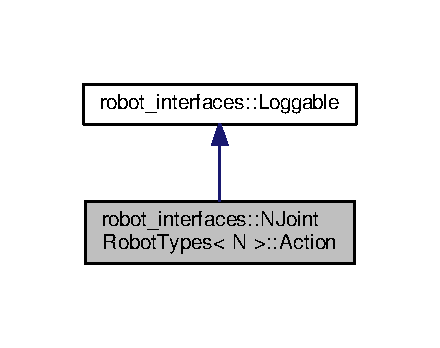
\includegraphics[width=211pt]{structrobot__interfaces_1_1NJointRobotTypes_1_1Action__inherit__graph}
\end{center}
\end{figure}


Collaboration diagram for robot\+\_\+interfaces\+:\+:N\+Joint\+Robot\+Types$<$ N $>$\+:\+:Action\+:
\nopagebreak
\begin{figure}[H]
\begin{center}
\leavevmode
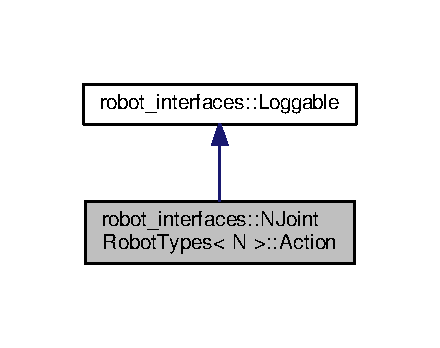
\includegraphics[width=211pt]{structrobot__interfaces_1_1NJointRobotTypes_1_1Action__coll__graph}
\end{center}
\end{figure}
\subsection*{Public Member Functions}
\begin{DoxyCompactItemize}
\item 
{\footnotesize template$<$class Archive $>$ }\\void {\bfseries serialize} (Archive \&archive)\hypertarget{structrobot__interfaces_1_1NJointRobotTypes_1_1Action_a7f645ab9be5cee75974d9cf1d4300c67}{}\label{structrobot__interfaces_1_1NJointRobotTypes_1_1Action_a7f645ab9be5cee75974d9cf1d4300c67}

\item 
std\+::vector$<$ std\+::string $>$ {\bfseries get\+\_\+name} () override\hypertarget{structrobot__interfaces_1_1NJointRobotTypes_1_1Action_a4d4b702fdf41cc9713c46edbbb26db51}{}\label{structrobot__interfaces_1_1NJointRobotTypes_1_1Action_a4d4b702fdf41cc9713c46edbbb26db51}

\item 
std\+::vector$<$ std\+::vector$<$ double $>$ $>$ {\bfseries get\+\_\+data} () override\hypertarget{structrobot__interfaces_1_1NJointRobotTypes_1_1Action_a8fe4c10c53d72e4f8bb9c09d3be9b39d}{}\label{structrobot__interfaces_1_1NJointRobotTypes_1_1Action_a8fe4c10c53d72e4f8bb9c09d3be9b39d}

\item 
\hyperlink{structrobot__interfaces_1_1NJointRobotTypes_1_1Action_aeb7fbd93adcc0140b5db42298211fe9d}{Action} (Vector \hyperlink{structrobot__interfaces_1_1NJointRobotTypes_1_1Action_ad19a93b677bdc60e655071743acf160e}{torque}=Vector\+::\+Zero(), Vector \hyperlink{structrobot__interfaces_1_1NJointRobotTypes_1_1Action_ad0d8104b1e521c7d0a316d093155e3a8}{position}=\hyperlink{structrobot__interfaces_1_1NJointRobotTypes_1_1Action_ab963d5faa78618bdaae53dc70ca936ae}{None}(), Vector \hyperlink{structrobot__interfaces_1_1NJointRobotTypes_1_1Action_a16eb24df6bdbc10c8ce08c0621723b92}{position\+\_\+kp}=\hyperlink{structrobot__interfaces_1_1NJointRobotTypes_1_1Action_ab963d5faa78618bdaae53dc70ca936ae}{None}(), Vector \hyperlink{structrobot__interfaces_1_1NJointRobotTypes_1_1Action_a3690aa864884fb51fb411d26eeea3fd4}{position\+\_\+kd}=\hyperlink{structrobot__interfaces_1_1NJointRobotTypes_1_1Action_ab963d5faa78618bdaae53dc70ca936ae}{None}())
\begin{DoxyCompactList}\small\item\em Create action with desired torque and (optional) position. \end{DoxyCompactList}\end{DoxyCompactItemize}
\subsection*{Static Public Member Functions}
\begin{DoxyCompactItemize}
\item 
static \hyperlink{structrobot__interfaces_1_1NJointRobotTypes_1_1Action}{Action} \hyperlink{structrobot__interfaces_1_1NJointRobotTypes_1_1Action_ae5aae444c808728af59a8a5b27035293}{Torque} (Vector \hyperlink{structrobot__interfaces_1_1NJointRobotTypes_1_1Action_ad19a93b677bdc60e655071743acf160e}{torque})
\begin{DoxyCompactList}\small\item\em Create an action that only contains a torque command. \end{DoxyCompactList}\item 
static \hyperlink{structrobot__interfaces_1_1NJointRobotTypes_1_1Action}{Action} \hyperlink{structrobot__interfaces_1_1NJointRobotTypes_1_1Action_ad60ea89acc73e544634b47a74797afd1}{Position} (Vector \hyperlink{structrobot__interfaces_1_1NJointRobotTypes_1_1Action_ad0d8104b1e521c7d0a316d093155e3a8}{position}, Vector kp=\hyperlink{structrobot__interfaces_1_1NJointRobotTypes_1_1Action_ab963d5faa78618bdaae53dc70ca936ae}{None}(), Vector kd=\hyperlink{structrobot__interfaces_1_1NJointRobotTypes_1_1Action_ab963d5faa78618bdaae53dc70ca936ae}{None}())
\begin{DoxyCompactList}\small\item\em Create an action that only contains a position command. \end{DoxyCompactList}\item 
static \hyperlink{structrobot__interfaces_1_1NJointRobotTypes_1_1Action}{Action} \hyperlink{structrobot__interfaces_1_1NJointRobotTypes_1_1Action_a076108da9106e45e9e8ab0b89e4c66e6}{Torque\+And\+Position} (Vector \hyperlink{structrobot__interfaces_1_1NJointRobotTypes_1_1Action_ad19a93b677bdc60e655071743acf160e}{torque}, Vector \hyperlink{structrobot__interfaces_1_1NJointRobotTypes_1_1Action_ad0d8104b1e521c7d0a316d093155e3a8}{position}, Vector \hyperlink{structrobot__interfaces_1_1NJointRobotTypes_1_1Action_a16eb24df6bdbc10c8ce08c0621723b92}{position\+\_\+kp}=\hyperlink{structrobot__interfaces_1_1NJointRobotTypes_1_1Action_ab963d5faa78618bdaae53dc70ca936ae}{None}(), Vector \hyperlink{structrobot__interfaces_1_1NJointRobotTypes_1_1Action_a3690aa864884fb51fb411d26eeea3fd4}{position\+\_\+kd}=\hyperlink{structrobot__interfaces_1_1NJointRobotTypes_1_1Action_ab963d5faa78618bdaae53dc70ca936ae}{None}())
\begin{DoxyCompactList}\small\item\em Create an action with both torque and position commands. \end{DoxyCompactList}\item 
static \hyperlink{structrobot__interfaces_1_1NJointRobotTypes_1_1Action}{Action} \hyperlink{structrobot__interfaces_1_1NJointRobotTypes_1_1Action_ad6fa1cd952afc4f02fcabc4221802b47}{Zero} ()
\begin{DoxyCompactList}\small\item\em Create a zero-\/torque action. \end{DoxyCompactList}\item 
static Vector \hyperlink{structrobot__interfaces_1_1NJointRobotTypes_1_1Action_ab963d5faa78618bdaae53dc70ca936ae}{None} ()
\begin{DoxyCompactList}\small\item\em Create a Na\+N-\/\+Vector. \end{DoxyCompactList}\end{DoxyCompactItemize}
\subsection*{Public Attributes}
\begin{DoxyCompactItemize}
\item 
Vector \hyperlink{structrobot__interfaces_1_1NJointRobotTypes_1_1Action_ad19a93b677bdc60e655071743acf160e}{torque}\hypertarget{structrobot__interfaces_1_1NJointRobotTypes_1_1Action_ad19a93b677bdc60e655071743acf160e}{}\label{structrobot__interfaces_1_1NJointRobotTypes_1_1Action_ad19a93b677bdc60e655071743acf160e}

\begin{DoxyCompactList}\small\item\em Desired torque command (in addition to position controller). \end{DoxyCompactList}\item 
Vector \hyperlink{structrobot__interfaces_1_1NJointRobotTypes_1_1Action_ad0d8104b1e521c7d0a316d093155e3a8}{position}\hypertarget{structrobot__interfaces_1_1NJointRobotTypes_1_1Action_ad0d8104b1e521c7d0a316d093155e3a8}{}\label{structrobot__interfaces_1_1NJointRobotTypes_1_1Action_ad0d8104b1e521c7d0a316d093155e3a8}

\begin{DoxyCompactList}\small\item\em Desired position. Set to NaN to disable position controller. \end{DoxyCompactList}\item 
Vector \hyperlink{structrobot__interfaces_1_1NJointRobotTypes_1_1Action_a16eb24df6bdbc10c8ce08c0621723b92}{position\+\_\+kp}\hypertarget{structrobot__interfaces_1_1NJointRobotTypes_1_1Action_a16eb24df6bdbc10c8ce08c0621723b92}{}\label{structrobot__interfaces_1_1NJointRobotTypes_1_1Action_a16eb24df6bdbc10c8ce08c0621723b92}

\begin{DoxyCompactList}\small\item\em P-\/gain for position controller. If NaN, default is used. \end{DoxyCompactList}\item 
Vector \hyperlink{structrobot__interfaces_1_1NJointRobotTypes_1_1Action_a3690aa864884fb51fb411d26eeea3fd4}{position\+\_\+kd}\hypertarget{structrobot__interfaces_1_1NJointRobotTypes_1_1Action_a3690aa864884fb51fb411d26eeea3fd4}{}\label{structrobot__interfaces_1_1NJointRobotTypes_1_1Action_a3690aa864884fb51fb411d26eeea3fd4}

\begin{DoxyCompactList}\small\item\em D-\/gain for position controller. If NaN, default is used. \end{DoxyCompactList}\end{DoxyCompactItemize}


\subsection{Constructor \& Destructor Documentation}
\index{robot\+\_\+interfaces\+::\+N\+Joint\+Robot\+Types\+::\+Action@{robot\+\_\+interfaces\+::\+N\+Joint\+Robot\+Types\+::\+Action}!Action@{Action}}
\index{Action@{Action}!robot\+\_\+interfaces\+::\+N\+Joint\+Robot\+Types\+::\+Action@{robot\+\_\+interfaces\+::\+N\+Joint\+Robot\+Types\+::\+Action}}
\subsubsection[{\texorpdfstring{Action(\+Vector torque=\+Vector\+::\+Zero(), Vector position=\+None(), Vector position\+\_\+kp=\+None(), Vector position\+\_\+kd=\+None())}{Action(Vector torque=Vector::Zero(), Vector position=None(), Vector position_kp=None(), Vector position_kd=None())}}]{\setlength{\rightskip}{0pt plus 5cm}template$<$size\+\_\+t N$>$ {\bf robot\+\_\+interfaces\+::\+N\+Joint\+Robot\+Types}$<$ N $>$\+::Action\+::\+Action (
\begin{DoxyParamCaption}
\item[{Vector}]{torque = {\ttfamily Vector\+:\+:Zero()}, }
\item[{Vector}]{position = {\ttfamily {\bf None}()}, }
\item[{Vector}]{position\+\_\+kp = {\ttfamily {\bf None}()}, }
\item[{Vector}]{position\+\_\+kd = {\ttfamily {\bf None}()}}
\end{DoxyParamCaption}
)\hspace{0.3cm}{\ttfamily [inline]}}\hypertarget{structrobot__interfaces_1_1NJointRobotTypes_1_1Action_aeb7fbd93adcc0140b5db42298211fe9d}{}\label{structrobot__interfaces_1_1NJointRobotTypes_1_1Action_aeb7fbd93adcc0140b5db42298211fe9d}


Create action with desired torque and (optional) position. 

The resulting torque command sent to the robot is \begin{DoxyVerb}sent_torque = torque + PD(position)
\end{DoxyVerb}


To disable the position controller, set the target position to NaN. The controller is executed joint-\/wise, so it is possible to run it only for some joints by setting a target position for these joints and setting the others to NaN.

The specified torque is always added to the result of the position controller, so if you only want to run the position controller, make sure to set {\ttfamily torque} to zero for all joints.

For more explicit code, the static factory methods {\ttfamily Troque}, {\ttfamily Position}, {\ttfamily Torque\+And\+Position} and {\ttfamily Zero} should be used instead directly creating actions through this constuctor.


\begin{DoxyParams}{Parameters}
{\em torque} & Desired torque. \\
\hline
{\em position} & Desired position. Set values to NaN to disable position controller for the corresponding joints \\
\hline
{\em position\+\_\+kp} & P-\/gains for the position controller. Set to NaN to use default values. \\
\hline
{\em position\+\_\+kd} & D-\/gains for the position controller. Set to NaN to use default values. \\
\hline
\end{DoxyParams}


\subsection{Member Function Documentation}
\index{robot\+\_\+interfaces\+::\+N\+Joint\+Robot\+Types\+::\+Action@{robot\+\_\+interfaces\+::\+N\+Joint\+Robot\+Types\+::\+Action}!None@{None}}
\index{None@{None}!robot\+\_\+interfaces\+::\+N\+Joint\+Robot\+Types\+::\+Action@{robot\+\_\+interfaces\+::\+N\+Joint\+Robot\+Types\+::\+Action}}
\subsubsection[{\texorpdfstring{None()}{None()}}]{\setlength{\rightskip}{0pt plus 5cm}template$<$size\+\_\+t N$>$ static Vector {\bf robot\+\_\+interfaces\+::\+N\+Joint\+Robot\+Types}$<$ N $>$\+::Action\+::\+None (
\begin{DoxyParamCaption}
{}
\end{DoxyParamCaption}
)\hspace{0.3cm}{\ttfamily [inline]}, {\ttfamily [static]}}\hypertarget{structrobot__interfaces_1_1NJointRobotTypes_1_1Action_ab963d5faa78618bdaae53dc70ca936ae}{}\label{structrobot__interfaces_1_1NJointRobotTypes_1_1Action_ab963d5faa78618bdaae53dc70ca936ae}


Create a Na\+N-\/\+Vector. 

Helper function to set defaults for position.

\begin{DoxyReturn}{Returns}
Vector with all elements set to NaN. 
\end{DoxyReturn}
\index{robot\+\_\+interfaces\+::\+N\+Joint\+Robot\+Types\+::\+Action@{robot\+\_\+interfaces\+::\+N\+Joint\+Robot\+Types\+::\+Action}!Position@{Position}}
\index{Position@{Position}!robot\+\_\+interfaces\+::\+N\+Joint\+Robot\+Types\+::\+Action@{robot\+\_\+interfaces\+::\+N\+Joint\+Robot\+Types\+::\+Action}}
\subsubsection[{\texorpdfstring{Position(\+Vector position, Vector kp=\+None(), Vector kd=\+None())}{Position(Vector position, Vector kp=None(), Vector kd=None())}}]{\setlength{\rightskip}{0pt plus 5cm}template$<$size\+\_\+t N$>$ static {\bf Action} {\bf robot\+\_\+interfaces\+::\+N\+Joint\+Robot\+Types}$<$ N $>$\+::Action\+::\+Position (
\begin{DoxyParamCaption}
\item[{Vector}]{position, }
\item[{Vector}]{kp = {\ttfamily {\bf None}()}, }
\item[{Vector}]{kd = {\ttfamily {\bf None}()}}
\end{DoxyParamCaption}
)\hspace{0.3cm}{\ttfamily [inline]}, {\ttfamily [static]}}\hypertarget{structrobot__interfaces_1_1NJointRobotTypes_1_1Action_ad60ea89acc73e544634b47a74797afd1}{}\label{structrobot__interfaces_1_1NJointRobotTypes_1_1Action_ad60ea89acc73e544634b47a74797afd1}


Create an action that only contains a position command. 


\begin{DoxyParams}{Parameters}
{\em position} & Desired position. \\
\hline
{\em kp} & P-\/gain for position controller. If not set, default is used. Set to NaN for specific joints to use default for this joint. \\
\hline
{\em kd} & D-\/gain for position controller. If not set, default is used. Set to NaN for specific joints to use default for this joint.\\
\hline
\end{DoxyParams}
\begin{DoxyReturn}{Returns}
Pure \char`\"{}position action\char`\"{}. 
\end{DoxyReturn}
\index{robot\+\_\+interfaces\+::\+N\+Joint\+Robot\+Types\+::\+Action@{robot\+\_\+interfaces\+::\+N\+Joint\+Robot\+Types\+::\+Action}!Torque@{Torque}}
\index{Torque@{Torque}!robot\+\_\+interfaces\+::\+N\+Joint\+Robot\+Types\+::\+Action@{robot\+\_\+interfaces\+::\+N\+Joint\+Robot\+Types\+::\+Action}}
\subsubsection[{\texorpdfstring{Torque(\+Vector torque)}{Torque(Vector torque)}}]{\setlength{\rightskip}{0pt plus 5cm}template$<$size\+\_\+t N$>$ static {\bf Action} {\bf robot\+\_\+interfaces\+::\+N\+Joint\+Robot\+Types}$<$ N $>$\+::Action\+::\+Torque (
\begin{DoxyParamCaption}
\item[{Vector}]{torque}
\end{DoxyParamCaption}
)\hspace{0.3cm}{\ttfamily [inline]}, {\ttfamily [static]}}\hypertarget{structrobot__interfaces_1_1NJointRobotTypes_1_1Action_ae5aae444c808728af59a8a5b27035293}{}\label{structrobot__interfaces_1_1NJointRobotTypes_1_1Action_ae5aae444c808728af59a8a5b27035293}


Create an action that only contains a torque command. 


\begin{DoxyParams}{Parameters}
{\em torque} & Desired torque.\\
\hline
\end{DoxyParams}
\begin{DoxyReturn}{Returns}
Pure \char`\"{}torque action\char`\"{}. 
\end{DoxyReturn}
\index{robot\+\_\+interfaces\+::\+N\+Joint\+Robot\+Types\+::\+Action@{robot\+\_\+interfaces\+::\+N\+Joint\+Robot\+Types\+::\+Action}!Torque\+And\+Position@{Torque\+And\+Position}}
\index{Torque\+And\+Position@{Torque\+And\+Position}!robot\+\_\+interfaces\+::\+N\+Joint\+Robot\+Types\+::\+Action@{robot\+\_\+interfaces\+::\+N\+Joint\+Robot\+Types\+::\+Action}}
\subsubsection[{\texorpdfstring{Torque\+And\+Position(\+Vector torque, Vector position, Vector position\+\_\+kp=\+None(), Vector position\+\_\+kd=\+None())}{TorqueAndPosition(Vector torque, Vector position, Vector position_kp=None(), Vector position_kd=None())}}]{\setlength{\rightskip}{0pt plus 5cm}template$<$size\+\_\+t N$>$ static {\bf Action} {\bf robot\+\_\+interfaces\+::\+N\+Joint\+Robot\+Types}$<$ N $>$\+::Action\+::\+Torque\+And\+Position (
\begin{DoxyParamCaption}
\item[{Vector}]{torque, }
\item[{Vector}]{position, }
\item[{Vector}]{position\+\_\+kp = {\ttfamily {\bf None}()}, }
\item[{Vector}]{position\+\_\+kd = {\ttfamily {\bf None}()}}
\end{DoxyParamCaption}
)\hspace{0.3cm}{\ttfamily [inline]}, {\ttfamily [static]}}\hypertarget{structrobot__interfaces_1_1NJointRobotTypes_1_1Action_a076108da9106e45e9e8ab0b89e4c66e6}{}\label{structrobot__interfaces_1_1NJointRobotTypes_1_1Action_a076108da9106e45e9e8ab0b89e4c66e6}


Create an action with both torque and position commands. 


\begin{DoxyParams}{Parameters}
{\em torque} & Desired torque. \\
\hline
{\em position} & Desired position. Set to NaN for specific joints to disable position control for this joint. \\
\hline
{\em kp} & P-\/gain for position controller. If not set, default is used. Set to NaN for specific joints to use default for this joint. \\
\hline
{\em kd} & D-\/gain for position controller. If not set, default is used. Set to NaN for specific joints to use default for this joint.\\
\hline
\end{DoxyParams}
\begin{DoxyReturn}{Returns}
\hyperlink{structrobot__interfaces_1_1NJointRobotTypes_1_1Action}{Action} with both torque and position commands. 
\end{DoxyReturn}
\index{robot\+\_\+interfaces\+::\+N\+Joint\+Robot\+Types\+::\+Action@{robot\+\_\+interfaces\+::\+N\+Joint\+Robot\+Types\+::\+Action}!Zero@{Zero}}
\index{Zero@{Zero}!robot\+\_\+interfaces\+::\+N\+Joint\+Robot\+Types\+::\+Action@{robot\+\_\+interfaces\+::\+N\+Joint\+Robot\+Types\+::\+Action}}
\subsubsection[{\texorpdfstring{Zero()}{Zero()}}]{\setlength{\rightskip}{0pt plus 5cm}template$<$size\+\_\+t N$>$ static {\bf Action} {\bf robot\+\_\+interfaces\+::\+N\+Joint\+Robot\+Types}$<$ N $>$\+::Action\+::\+Zero (
\begin{DoxyParamCaption}
{}
\end{DoxyParamCaption}
)\hspace{0.3cm}{\ttfamily [inline]}, {\ttfamily [static]}}\hypertarget{structrobot__interfaces_1_1NJointRobotTypes_1_1Action_ad6fa1cd952afc4f02fcabc4221802b47}{}\label{structrobot__interfaces_1_1NJointRobotTypes_1_1Action_ad6fa1cd952afc4f02fcabc4221802b47}


Create a zero-\/torque action. 

\begin{DoxyReturn}{Returns}
Zero-\/torque action with position control disabled. 
\end{DoxyReturn}


The documentation for this struct was generated from the following file\+:\begin{DoxyCompactItemize}
\item 
include/robot\+\_\+interfaces/n\+\_\+joint\+\_\+robot\+\_\+types.\+hpp\end{DoxyCompactItemize}

\hypertarget{classDriver}{}\section{Driver Class Reference}
\label{classDriver}\index{Driver@{Driver}}


Inheritance diagram for Driver\+:
\nopagebreak
\begin{figure}[H]
\begin{center}
\leavevmode
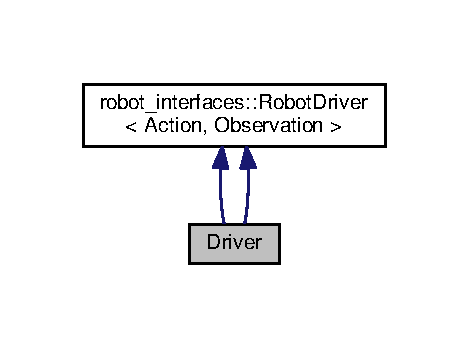
\includegraphics[width=225pt]{classDriver__inherit__graph}
\end{center}
\end{figure}


Collaboration diagram for Driver\+:
\nopagebreak
\begin{figure}[H]
\begin{center}
\leavevmode
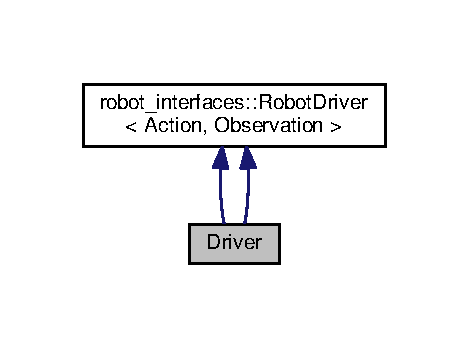
\includegraphics[width=225pt]{classDriver__coll__graph}
\end{center}
\end{figure}
\subsection*{Public Member Functions}
\begin{DoxyCompactItemize}
\item 
{\bfseries Driver} (int min, int max)\hypertarget{classDriver_a440406bbabc606d80051e93b44b1bd2e}{}\label{classDriver_a440406bbabc606d80051e93b44b1bd2e}

\item 
void \hyperlink{classDriver_a81c0beb523fad80cd40cfcc6a6e3de2d}{initialize} ()
\begin{DoxyCompactList}\small\item\em Initialize the robot. \end{DoxyCompactList}\item 
\hyperlink{classAction}{Action} \hyperlink{classDriver_a0f8d51bef151ccc38a0cb7b226048e28}{apply\+\_\+action} (const \hyperlink{classAction}{Action} \&action\+\_\+to\+\_\+apply)
\begin{DoxyCompactList}\small\item\em Apply action immediately and block until it is executed. \end{DoxyCompactList}\item 
\hyperlink{classObservation}{Observation} \hyperlink{classDriver_afb09663997bffc5c694fb5aa8aca243a}{get\+\_\+latest\+\_\+observation} ()
\begin{DoxyCompactList}\small\item\em Return the latest observation immediately. \end{DoxyCompactList}\item 
std\+::string \hyperlink{classDriver_a6fb739b87c892c4102e838508855c0be}{get\+\_\+error} ()
\begin{DoxyCompactList}\small\item\em Get error message if there is any error. \end{DoxyCompactList}\item 
void \hyperlink{classDriver_a630fc9183eb419beb09b5828b4547b6d}{shutdown} ()\hypertarget{classDriver_a630fc9183eb419beb09b5828b4547b6d}{}\label{classDriver_a630fc9183eb419beb09b5828b4547b6d}

\begin{DoxyCompactList}\small\item\em Shut down the robot safely. \end{DoxyCompactList}\item 
void \hyperlink{classDriver_a81c0beb523fad80cd40cfcc6a6e3de2d}{initialize} ()
\begin{DoxyCompactList}\small\item\em Initialize the robot. \end{DoxyCompactList}\item 
\hyperlink{classAction}{Action} \hyperlink{classDriver_a0f8d51bef151ccc38a0cb7b226048e28}{apply\+\_\+action} (const \hyperlink{classAction}{Action} \&action\+\_\+to\+\_\+apply)
\begin{DoxyCompactList}\small\item\em Apply action immediately and block until it is executed. \end{DoxyCompactList}\item 
\hyperlink{classObservation}{Observation} \hyperlink{classDriver_afb09663997bffc5c694fb5aa8aca243a}{get\+\_\+latest\+\_\+observation} ()
\begin{DoxyCompactList}\small\item\em Return the latest observation immediately. \end{DoxyCompactList}\item 
std\+::string \hyperlink{classDriver_a6fb739b87c892c4102e838508855c0be}{get\+\_\+error} ()
\begin{DoxyCompactList}\small\item\em Get error message if there is any error. \end{DoxyCompactList}\item 
void \hyperlink{classDriver_a630fc9183eb419beb09b5828b4547b6d}{shutdown} ()\hypertarget{classDriver_a630fc9183eb419beb09b5828b4547b6d}{}\label{classDriver_a630fc9183eb419beb09b5828b4547b6d}

\begin{DoxyCompactList}\small\item\em Shut down the robot safely. \end{DoxyCompactList}\end{DoxyCompactItemize}
\subsection*{Private Attributes}
\begin{DoxyCompactItemize}
\item 
int {\bfseries state\+\_\+} \mbox{[}2\mbox{]}\hypertarget{classDriver_ac342821e039cd6e64c8227e5fd2f10c7}{}\label{classDriver_ac342821e039cd6e64c8227e5fd2f10c7}

\item 
int {\bfseries min\+\_\+}\hypertarget{classDriver_ae1f5333762d8c70fd5e8afc0314d3568}{}\label{classDriver_ae1f5333762d8c70fd5e8afc0314d3568}

\item 
int {\bfseries max\+\_\+}\hypertarget{classDriver_a9292f94b9df62ede6d983824ff79480c}{}\label{classDriver_a9292f94b9df62ede6d983824ff79480c}

\end{DoxyCompactItemize}
\subsection*{Static Private Attributes}
\begin{DoxyCompactItemize}
\item 
static const int {\bfseries M\+AX} = 1000\hypertarget{classDriver_a2f75d16f4af650ca9cf1cdd8b653cc18}{}\label{classDriver_a2f75d16f4af650ca9cf1cdd8b653cc18}

\item 
static const int {\bfseries M\+IN} = 0\hypertarget{classDriver_a09b06e92e4ea9df756e3b6e038fa25f6}{}\label{classDriver_a09b06e92e4ea9df756e3b6e038fa25f6}

\end{DoxyCompactItemize}
\subsection*{Additional Inherited Members}


\subsection{Detailed Description}
\begin{Desc}
\item[Examples\+: ]\par
\hyperlink{demo_8cpp-example}{demo.\+cpp}, and \hyperlink{demo_multiprocess_backend_8cpp-example}{demo\+\_\+multiprocess\+\_\+backend.\+cpp}.\end{Desc}


\subsection{Member Function Documentation}
\index{Driver@{Driver}!apply\+\_\+action@{apply\+\_\+action}}
\index{apply\+\_\+action@{apply\+\_\+action}!Driver@{Driver}}
\subsubsection[{\texorpdfstring{apply\+\_\+action(const Action \&action\+\_\+to\+\_\+apply)}{apply_action(const Action &action_to_apply)}}]{\setlength{\rightskip}{0pt plus 5cm}{\bf Action} Driver\+::apply\+\_\+action (
\begin{DoxyParamCaption}
\item[{const {\bf Action} \&}]{desired\+\_\+action}
\end{DoxyParamCaption}
)\hspace{0.3cm}{\ttfamily [inline]}, {\ttfamily [virtual]}}\hypertarget{classDriver_a0f8d51bef151ccc38a0cb7b226048e28}{}\label{classDriver_a0f8d51bef151ccc38a0cb7b226048e28}


Apply action immediately and block until it is executed. 

This method must apply the desired\+\_\+action immediately when it is called, and only return once the action has been executed completely. This way we can accommodate both simulators and real robots with this interface.


\begin{DoxyParams}{Parameters}
{\em desired\+\_\+action} & The action we want to apply. \\
\hline
\end{DoxyParams}
\begin{DoxyReturn}{Returns}
The action that was actually applied (since due to safety reasons it might not be possible to apply the desired action). 
\end{DoxyReturn}


Implements \hyperlink{classrobot__interfaces_1_1RobotDriver_a4294e522fcd12b38d69f7d53fae5d74a}{robot\+\_\+interfaces\+::\+Robot\+Driver$<$ Action, Observation $>$}.

\index{Driver@{Driver}!apply\+\_\+action@{apply\+\_\+action}}
\index{apply\+\_\+action@{apply\+\_\+action}!Driver@{Driver}}
\subsubsection[{\texorpdfstring{apply\+\_\+action(const Action \&action\+\_\+to\+\_\+apply)}{apply_action(const Action &action_to_apply)}}]{\setlength{\rightskip}{0pt plus 5cm}{\bf Action} Driver\+::apply\+\_\+action (
\begin{DoxyParamCaption}
\item[{const {\bf Action} \&}]{desired\+\_\+action}
\end{DoxyParamCaption}
)\hspace{0.3cm}{\ttfamily [inline]}, {\ttfamily [virtual]}}\hypertarget{classDriver_a0f8d51bef151ccc38a0cb7b226048e28}{}\label{classDriver_a0f8d51bef151ccc38a0cb7b226048e28}


Apply action immediately and block until it is executed. 

This method must apply the desired\+\_\+action immediately when it is called, and only return once the action has been executed completely. This way we can accommodate both simulators and real robots with this interface.


\begin{DoxyParams}{Parameters}
{\em desired\+\_\+action} & The action we want to apply. \\
\hline
\end{DoxyParams}
\begin{DoxyReturn}{Returns}
The action that was actually applied (since due to safety reasons it might not be possible to apply the desired action). 
\end{DoxyReturn}


Implements \hyperlink{classrobot__interfaces_1_1RobotDriver_a4294e522fcd12b38d69f7d53fae5d74a}{robot\+\_\+interfaces\+::\+Robot\+Driver$<$ Action, Observation $>$}.

\index{Driver@{Driver}!get\+\_\+error@{get\+\_\+error}}
\index{get\+\_\+error@{get\+\_\+error}!Driver@{Driver}}
\subsubsection[{\texorpdfstring{get\+\_\+error()}{get_error()}}]{\setlength{\rightskip}{0pt plus 5cm}std\+::string Driver\+::get\+\_\+error (
\begin{DoxyParamCaption}
{}
\end{DoxyParamCaption}
)\hspace{0.3cm}{\ttfamily [inline]}, {\ttfamily [virtual]}}\hypertarget{classDriver_a6fb739b87c892c4102e838508855c0be}{}\label{classDriver_a6fb739b87c892c4102e838508855c0be}


Get error message if there is any error. 

\begin{DoxyReturn}{Returns}
Returns an error message or an empty string if there is no error. 
\end{DoxyReturn}


Implements \hyperlink{classrobot__interfaces_1_1RobotDriver_acdf4c5d6993b836a180e6b6fc12b3445}{robot\+\_\+interfaces\+::\+Robot\+Driver$<$ Action, Observation $>$}.

\index{Driver@{Driver}!get\+\_\+error@{get\+\_\+error}}
\index{get\+\_\+error@{get\+\_\+error}!Driver@{Driver}}
\subsubsection[{\texorpdfstring{get\+\_\+error()}{get_error()}}]{\setlength{\rightskip}{0pt plus 5cm}std\+::string Driver\+::get\+\_\+error (
\begin{DoxyParamCaption}
{}
\end{DoxyParamCaption}
)\hspace{0.3cm}{\ttfamily [inline]}, {\ttfamily [virtual]}}\hypertarget{classDriver_a6fb739b87c892c4102e838508855c0be}{}\label{classDriver_a6fb739b87c892c4102e838508855c0be}


Get error message if there is any error. 

\begin{DoxyReturn}{Returns}
Returns an error message or an empty string if there is no error. 
\end{DoxyReturn}


Implements \hyperlink{classrobot__interfaces_1_1RobotDriver_acdf4c5d6993b836a180e6b6fc12b3445}{robot\+\_\+interfaces\+::\+Robot\+Driver$<$ Action, Observation $>$}.

\index{Driver@{Driver}!get\+\_\+latest\+\_\+observation@{get\+\_\+latest\+\_\+observation}}
\index{get\+\_\+latest\+\_\+observation@{get\+\_\+latest\+\_\+observation}!Driver@{Driver}}
\subsubsection[{\texorpdfstring{get\+\_\+latest\+\_\+observation()}{get_latest_observation()}}]{\setlength{\rightskip}{0pt plus 5cm}{\bf Observation} Driver\+::get\+\_\+latest\+\_\+observation (
\begin{DoxyParamCaption}
{}
\end{DoxyParamCaption}
)\hspace{0.3cm}{\ttfamily [inline]}, {\ttfamily [virtual]}}\hypertarget{classDriver_afb09663997bffc5c694fb5aa8aca243a}{}\label{classDriver_afb09663997bffc5c694fb5aa8aca243a}


Return the latest observation immediately. 

\begin{DoxyReturn}{Returns}
\hyperlink{classObservation}{Observation} 
\end{DoxyReturn}


Implements \hyperlink{classrobot__interfaces_1_1RobotDriver_ad13d4f4fdfe78bdde4fc964f07fa45e2}{robot\+\_\+interfaces\+::\+Robot\+Driver$<$ Action, Observation $>$}.

\index{Driver@{Driver}!get\+\_\+latest\+\_\+observation@{get\+\_\+latest\+\_\+observation}}
\index{get\+\_\+latest\+\_\+observation@{get\+\_\+latest\+\_\+observation}!Driver@{Driver}}
\subsubsection[{\texorpdfstring{get\+\_\+latest\+\_\+observation()}{get_latest_observation()}}]{\setlength{\rightskip}{0pt plus 5cm}{\bf Observation} Driver\+::get\+\_\+latest\+\_\+observation (
\begin{DoxyParamCaption}
{}
\end{DoxyParamCaption}
)\hspace{0.3cm}{\ttfamily [inline]}, {\ttfamily [virtual]}}\hypertarget{classDriver_afb09663997bffc5c694fb5aa8aca243a}{}\label{classDriver_afb09663997bffc5c694fb5aa8aca243a}


Return the latest observation immediately. 

\begin{DoxyReturn}{Returns}
\hyperlink{classObservation}{Observation} 
\end{DoxyReturn}


Implements \hyperlink{classrobot__interfaces_1_1RobotDriver_ad13d4f4fdfe78bdde4fc964f07fa45e2}{robot\+\_\+interfaces\+::\+Robot\+Driver$<$ Action, Observation $>$}.

\index{Driver@{Driver}!initialize@{initialize}}
\index{initialize@{initialize}!Driver@{Driver}}
\subsubsection[{\texorpdfstring{initialize()}{initialize()}}]{\setlength{\rightskip}{0pt plus 5cm}void Driver\+::initialize (
\begin{DoxyParamCaption}
{}
\end{DoxyParamCaption}
)\hspace{0.3cm}{\ttfamily [inline]}, {\ttfamily [virtual]}}\hypertarget{classDriver_a81c0beb523fad80cd40cfcc6a6e3de2d}{}\label{classDriver_a81c0beb523fad80cd40cfcc6a6e3de2d}


Initialize the robot. 

Any initialization procedures that need to be done before sending actions to the robot should be done in this method (e.\+g. homing to find the absolute position). 

Implements \hyperlink{classrobot__interfaces_1_1RobotDriver_af3cbef570a455e1f8085d701282264ff}{robot\+\_\+interfaces\+::\+Robot\+Driver$<$ Action, Observation $>$}.

\index{Driver@{Driver}!initialize@{initialize}}
\index{initialize@{initialize}!Driver@{Driver}}
\subsubsection[{\texorpdfstring{initialize()}{initialize()}}]{\setlength{\rightskip}{0pt plus 5cm}void Driver\+::initialize (
\begin{DoxyParamCaption}
{}
\end{DoxyParamCaption}
)\hspace{0.3cm}{\ttfamily [inline]}, {\ttfamily [virtual]}}\hypertarget{classDriver_a81c0beb523fad80cd40cfcc6a6e3de2d}{}\label{classDriver_a81c0beb523fad80cd40cfcc6a6e3de2d}


Initialize the robot. 

Any initialization procedures that need to be done before sending actions to the robot should be done in this method (e.\+g. homing to find the absolute position). 

Implements \hyperlink{classrobot__interfaces_1_1RobotDriver_af3cbef570a455e1f8085d701282264ff}{robot\+\_\+interfaces\+::\+Robot\+Driver$<$ Action, Observation $>$}.



The documentation for this class was generated from the following files\+:\begin{DoxyCompactItemize}
\item 
demos/\hyperlink{demo_8cpp}{demo.\+cpp}\item 
demos/\hyperlink{demo__multiprocess__backend_8cpp}{demo\+\_\+multiprocess\+\_\+backend.\+cpp}\end{DoxyCompactItemize}

\hypertarget{structrobot__interfaces_1_1FingerTypes}{}\section{robot\+\_\+interfaces\+:\+:Finger\+Types Struct Reference}
\label{structrobot__interfaces_1_1FingerTypes}\index{robot\+\_\+interfaces\+::\+Finger\+Types@{robot\+\_\+interfaces\+::\+Finger\+Types}}


Types for the Finger robot (basic 3-\/joint robot).  




{\ttfamily \#include $<$finger\+\_\+types.\+hpp$>$}



Inheritance diagram for robot\+\_\+interfaces\+:\+:Finger\+Types\+:
\nopagebreak
\begin{figure}[H]
\begin{center}
\leavevmode
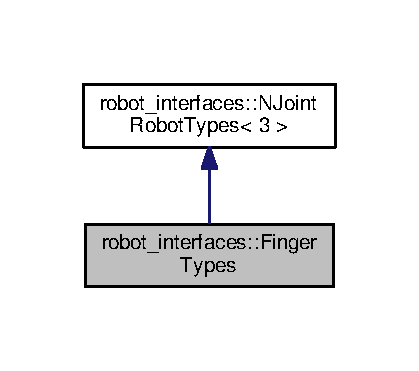
\includegraphics[width=201pt]{structrobot__interfaces_1_1FingerTypes__inherit__graph}
\end{center}
\end{figure}


Collaboration diagram for robot\+\_\+interfaces\+:\+:Finger\+Types\+:
\nopagebreak
\begin{figure}[H]
\begin{center}
\leavevmode
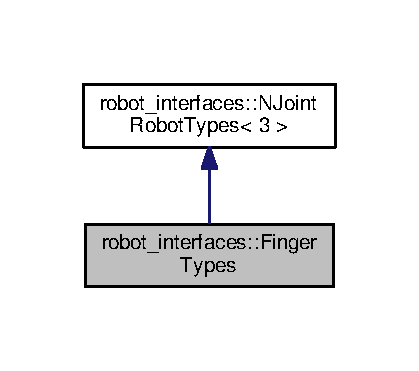
\includegraphics[width=201pt]{structrobot__interfaces_1_1FingerTypes__coll__graph}
\end{center}
\end{figure}
\subsection*{Additional Inherited Members}


\subsection{Detailed Description}
Types for the Finger robot (basic 3-\/joint robot). 

The documentation for this struct was generated from the following file\+:\begin{DoxyCompactItemize}
\item 
include/robot\+\_\+interfaces/finger\+\_\+types.\+hpp\end{DoxyCompactItemize}

\hypertarget{classrobot__interfaces_1_1GlobalSignalHandler}{}\section{robot\+\_\+interfaces\+:\+:Global\+Signal\+Handler Class Reference}
\label{classrobot__interfaces_1_1GlobalSignalHandler}\index{robot\+\_\+interfaces\+::\+Global\+Signal\+Handler@{robot\+\_\+interfaces\+::\+Global\+Signal\+Handler}}


Static class implementing a signal handler and providing information about S\+I\+G\+I\+NT.  




{\ttfamily \#include $<$global\+\_\+signal\+\_\+handler.\+hpp$>$}

\subsection*{Static Public Member Functions}
\begin{DoxyCompactItemize}
\item 
static void \hyperlink{classrobot__interfaces_1_1GlobalSignalHandler_af7503f0022d78843f85062d7b602fe4b}{initialize} ()
\begin{DoxyCompactList}\small\item\em Initialize the signal handler. \end{DoxyCompactList}\item 
static void \hyperlink{classrobot__interfaces_1_1GlobalSignalHandler_a55da931218f7d10052c233832456c601}{signal\+\_\+handler} (int signal)\hypertarget{classrobot__interfaces_1_1GlobalSignalHandler_a55da931218f7d10052c233832456c601}{}\label{classrobot__interfaces_1_1GlobalSignalHandler_a55da931218f7d10052c233832456c601}

\begin{DoxyCompactList}\small\item\em Handles the signals. Do not call this directly. \end{DoxyCompactList}\item 
static bool \hyperlink{classrobot__interfaces_1_1GlobalSignalHandler_a7d24e6a71be9282a270e92be4e3808b9}{has\+\_\+received\+\_\+sigint} ()
\begin{DoxyCompactList}\small\item\em Check if a S\+I\+G\+I\+NT was received. \end{DoxyCompactList}\end{DoxyCompactItemize}
\subsection*{Static Private Attributes}
\begin{DoxyCompactItemize}
\item 
static bool {\bfseries received\+\_\+sigint\+\_\+} = false\hypertarget{classrobot__interfaces_1_1GlobalSignalHandler_ae0c579060c4b33139ed9f23c6398fe01}{}\label{classrobot__interfaces_1_1GlobalSignalHandler_ae0c579060c4b33139ed9f23c6398fe01}

\end{DoxyCompactItemize}


\subsection{Detailed Description}
Static class implementing a signal handler and providing information about S\+I\+G\+I\+NT. 

Since signal handlers cannot be implemented in a non-\/static class method, use this globally accessible class as a workaround. It registers a signal handler provides static methods to poll if certain signals are received. 

\subsection{Member Function Documentation}
\index{robot\+\_\+interfaces\+::\+Global\+Signal\+Handler@{robot\+\_\+interfaces\+::\+Global\+Signal\+Handler}!has\+\_\+received\+\_\+sigint@{has\+\_\+received\+\_\+sigint}}
\index{has\+\_\+received\+\_\+sigint@{has\+\_\+received\+\_\+sigint}!robot\+\_\+interfaces\+::\+Global\+Signal\+Handler@{robot\+\_\+interfaces\+::\+Global\+Signal\+Handler}}
\subsubsection[{\texorpdfstring{has\+\_\+received\+\_\+sigint()}{has_received_sigint()}}]{\setlength{\rightskip}{0pt plus 5cm}bool robot\+\_\+interfaces\+::\+Global\+Signal\+Handler\+::has\+\_\+received\+\_\+sigint (
\begin{DoxyParamCaption}
{}
\end{DoxyParamCaption}
)\hspace{0.3cm}{\ttfamily [static]}}\hypertarget{classrobot__interfaces_1_1GlobalSignalHandler_a7d24e6a71be9282a270e92be4e3808b9}{}\label{classrobot__interfaces_1_1GlobalSignalHandler_a7d24e6a71be9282a270e92be4e3808b9}


Check if a S\+I\+G\+I\+NT was received. 

\begin{DoxyReturn}{Returns}
True if S\+I\+G\+I\+NT was received. 
\end{DoxyReturn}
\index{robot\+\_\+interfaces\+::\+Global\+Signal\+Handler@{robot\+\_\+interfaces\+::\+Global\+Signal\+Handler}!initialize@{initialize}}
\index{initialize@{initialize}!robot\+\_\+interfaces\+::\+Global\+Signal\+Handler@{robot\+\_\+interfaces\+::\+Global\+Signal\+Handler}}
\subsubsection[{\texorpdfstring{initialize()}{initialize()}}]{\setlength{\rightskip}{0pt plus 5cm}void robot\+\_\+interfaces\+::\+Global\+Signal\+Handler\+::initialize (
\begin{DoxyParamCaption}
{}
\end{DoxyParamCaption}
)\hspace{0.3cm}{\ttfamily [static]}}\hypertarget{classrobot__interfaces_1_1GlobalSignalHandler_af7503f0022d78843f85062d7b602fe4b}{}\label{classrobot__interfaces_1_1GlobalSignalHandler_af7503f0022d78843f85062d7b602fe4b}


Initialize the signal handler. 

This must be called before using the class. Does nothing when called a second time. 

The documentation for this class was generated from the following files\+:\begin{DoxyCompactItemize}
\item 
include/robot\+\_\+interfaces/\hyperlink{global__signal__handler_8hpp}{global\+\_\+signal\+\_\+handler.\+hpp}\item 
src/\hyperlink{global__signal__handler_8cpp}{global\+\_\+signal\+\_\+handler.\+cpp}\end{DoxyCompactItemize}

\hypertarget{classrobot__interfaces_1_1Loggable}{}\section{robot\+\_\+interfaces\+:\+:Loggable Class Reference}
\label{classrobot__interfaces_1_1Loggable}\index{robot\+\_\+interfaces\+::\+Loggable@{robot\+\_\+interfaces\+::\+Loggable}}


Inheritance diagram for robot\+\_\+interfaces\+:\+:Loggable\+:
\nopagebreak
\begin{figure}[H]
\begin{center}
\leavevmode
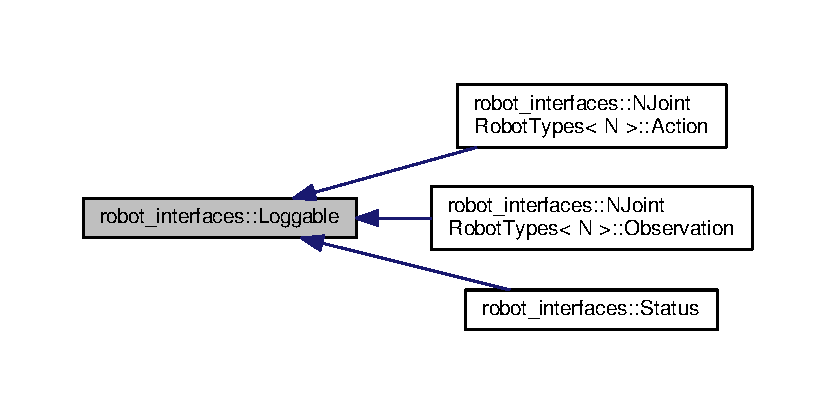
\includegraphics[width=350pt]{classrobot__interfaces_1_1Loggable__inherit__graph}
\end{center}
\end{figure}
\subsection*{Public Member Functions}
\begin{DoxyCompactItemize}
\item 
virtual std\+::vector$<$ std\+::string $>$ {\bfseries get\+\_\+name} ()=0\hypertarget{classrobot__interfaces_1_1Loggable_a19635ebc166379f11fe4c8e58153243a}{}\label{classrobot__interfaces_1_1Loggable_a19635ebc166379f11fe4c8e58153243a}

\item 
virtual std\+::vector$<$ std\+::vector$<$ double $>$ $>$ {\bfseries get\+\_\+data} ()=0\hypertarget{classrobot__interfaces_1_1Loggable_a28ffee45cf66a84d16b2c907ed10367c}{}\label{classrobot__interfaces_1_1Loggable_a28ffee45cf66a84d16b2c907ed10367c}

\end{DoxyCompactItemize}


The documentation for this class was generated from the following file\+:\begin{DoxyCompactItemize}
\item 
include/robot\+\_\+interfaces/loggable.\+hpp\end{DoxyCompactItemize}

\hypertarget{classrobot__interfaces_1_1MonitoredRobotDriver}{}\section{robot\+\_\+interfaces\+:\+:Monitored\+Robot\+Driver$<$ Driver $>$ Class Template Reference}
\label{classrobot__interfaces_1_1MonitoredRobotDriver}\index{robot\+\_\+interfaces\+::\+Monitored\+Robot\+Driver$<$ Driver $>$@{robot\+\_\+interfaces\+::\+Monitored\+Robot\+Driver$<$ Driver $>$}}


Wrapper for \hyperlink{classrobot__interfaces_1_1RobotDriver}{Robot\+Driver} that monitors timing.  




{\ttfamily \#include $<$monitored\+\_\+robot\+\_\+driver.\+hpp$>$}



Inheritance diagram for robot\+\_\+interfaces\+:\+:Monitored\+Robot\+Driver$<$ Driver $>$\+:
\nopagebreak
\begin{figure}[H]
\begin{center}
\leavevmode
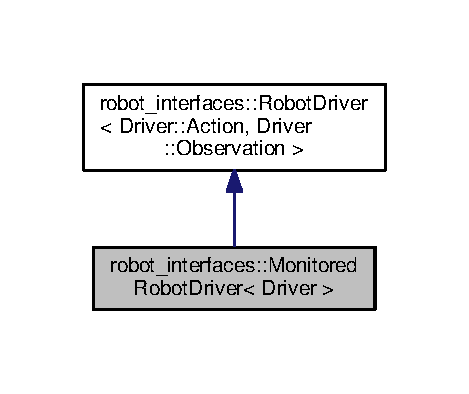
\includegraphics[width=225pt]{classrobot__interfaces_1_1MonitoredRobotDriver__inherit__graph}
\end{center}
\end{figure}


Collaboration diagram for robot\+\_\+interfaces\+:\+:Monitored\+Robot\+Driver$<$ Driver $>$\+:
\nopagebreak
\begin{figure}[H]
\begin{center}
\leavevmode
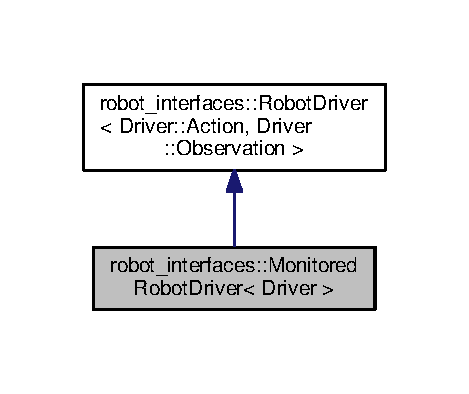
\includegraphics[width=225pt]{classrobot__interfaces_1_1MonitoredRobotDriver__coll__graph}
\end{center}
\end{figure}
\subsection*{Public Types}
\begin{DoxyCompactItemize}
\item 
typedef std\+::shared\+\_\+ptr$<$ \hyperlink{classDriver}{Driver} $>$ {\bfseries Robot\+Driver\+Ptr}\hypertarget{classrobot__interfaces_1_1MonitoredRobotDriver_a272fbf2c9bf93f568c00dd1e37e62e97}{}\label{classrobot__interfaces_1_1MonitoredRobotDriver_a272fbf2c9bf93f568c00dd1e37e62e97}

\end{DoxyCompactItemize}
\subsection*{Public Member Functions}
\begin{DoxyCompactItemize}
\item 
\hyperlink{classrobot__interfaces_1_1MonitoredRobotDriver_a2ea1456e85ad7596295cb047e552dc06}{Monitored\+Robot\+Driver} (Robot\+Driver\+Ptr robot\+\_\+driver, const double max\+\_\+action\+\_\+duration\+\_\+s, const double max\+\_\+inter\+\_\+action\+\_\+duration\+\_\+s)
\begin{DoxyCompactList}\small\item\em Starts a thread for monitoring timing of action execution. \end{DoxyCompactList}\item 
\hyperlink{classrobot__interfaces_1_1MonitoredRobotDriver_a07dfd2cc6f1dc07fad82914814a43188}{$\sim$\+Monitored\+Robot\+Driver} ()\hypertarget{classrobot__interfaces_1_1MonitoredRobotDriver_a07dfd2cc6f1dc07fad82914814a43188}{}\label{classrobot__interfaces_1_1MonitoredRobotDriver_a07dfd2cc6f1dc07fad82914814a43188}

\begin{DoxyCompactList}\small\item\em Shuts down the robot and stops the monitoring thread. \end{DoxyCompactList}\item 
virtual Driver\+::\+Action \hyperlink{classrobot__interfaces_1_1MonitoredRobotDriver_a3f0f7cbf74236e91d33dcfc08206b5e9}{apply\+\_\+action} (const typename Driver\+::\+Action \&desired\+\_\+action) final
\begin{DoxyCompactList}\small\item\em Apply desired action on the robot. \end{DoxyCompactList}\item 
virtual void \hyperlink{classrobot__interfaces_1_1MonitoredRobotDriver_a47b68c24afaa087e4e60e6413ab7ac89}{initialize} ()
\begin{DoxyCompactList}\small\item\em Initialize the robot. \end{DoxyCompactList}\item 
virtual Driver\+::\+Observation \hyperlink{classrobot__interfaces_1_1MonitoredRobotDriver_a97774dddcda1038f338d18ef0b572ad8}{get\+\_\+latest\+\_\+observation} ()
\begin{DoxyCompactList}\small\item\em Return the latest observation immediately. \end{DoxyCompactList}\item 
virtual std\+::string \hyperlink{classrobot__interfaces_1_1MonitoredRobotDriver_a944425cc7e0845184f33b16405a9e61e}{get\+\_\+error} ()
\begin{DoxyCompactList}\small\item\em Get error message if there is any error. \end{DoxyCompactList}\item 
virtual void \hyperlink{classrobot__interfaces_1_1MonitoredRobotDriver_a95714a60e69a3ac06461382a7b391289}{shutdown} () final
\begin{DoxyCompactList}\small\item\em Shut down the robot safely. \end{DoxyCompactList}\end{DoxyCompactItemize}
\subsection*{Private Member Functions}
\begin{DoxyCompactItemize}
\item 
void \hyperlink{classrobot__interfaces_1_1MonitoredRobotDriver_a6ed3d940dce484dcdc558a52a8dfe8a5}{loop} ()
\begin{DoxyCompactList}\small\item\em Monitor the timing of action execution. \end{DoxyCompactList}\end{DoxyCompactItemize}
\subsection*{Static Private Member Functions}
\begin{DoxyCompactItemize}
\item 
static void $\ast$ {\bfseries loop} (void $\ast$instance\+\_\+pointer)\hypertarget{classrobot__interfaces_1_1MonitoredRobotDriver_a46ddb0472196631d6cdd109f3753c693}{}\label{classrobot__interfaces_1_1MonitoredRobotDriver_a46ddb0472196631d6cdd109f3753c693}

\end{DoxyCompactItemize}
\subsection*{Private Attributes}
\begin{DoxyCompactItemize}
\item 
Robot\+Driver\+Ptr \hyperlink{classrobot__interfaces_1_1MonitoredRobotDriver_ae43540d38c9414d8ad734a9c88155a6e}{robot\+\_\+driver\+\_\+}\hypertarget{classrobot__interfaces_1_1MonitoredRobotDriver_ae43540d38c9414d8ad734a9c88155a6e}{}\label{classrobot__interfaces_1_1MonitoredRobotDriver_ae43540d38c9414d8ad734a9c88155a6e}

\begin{DoxyCompactList}\small\item\em The actual robot driver. \end{DoxyCompactList}\item 
double \hyperlink{classrobot__interfaces_1_1MonitoredRobotDriver_a860e5a4835a916faf08e1ab932b34bb1}{max\+\_\+action\+\_\+duration\+\_\+s\+\_\+}\hypertarget{classrobot__interfaces_1_1MonitoredRobotDriver_a860e5a4835a916faf08e1ab932b34bb1}{}\label{classrobot__interfaces_1_1MonitoredRobotDriver_a860e5a4835a916faf08e1ab932b34bb1}

\begin{DoxyCompactList}\small\item\em Max. time for executing an action. \end{DoxyCompactList}\item 
double \hyperlink{classrobot__interfaces_1_1MonitoredRobotDriver_acef35c51b51f1d05453b5b672f43a516}{max\+\_\+inter\+\_\+action\+\_\+duration\+\_\+s\+\_\+}\hypertarget{classrobot__interfaces_1_1MonitoredRobotDriver_acef35c51b51f1d05453b5b672f43a516}{}\label{classrobot__interfaces_1_1MonitoredRobotDriver_acef35c51b51f1d05453b5b672f43a516}

\begin{DoxyCompactList}\small\item\em Max. idle time between actions. \end{DoxyCompactList}\item 
std\+::atomic$<$ bool $>$ \hyperlink{classrobot__interfaces_1_1MonitoredRobotDriver_a8200e14e4d9e4d1d8c2fc4e0134cf7cd}{is\+\_\+shutdown\+\_\+}\hypertarget{classrobot__interfaces_1_1MonitoredRobotDriver_a8200e14e4d9e4d1d8c2fc4e0134cf7cd}{}\label{classrobot__interfaces_1_1MonitoredRobotDriver_a8200e14e4d9e4d1d8c2fc4e0134cf7cd}

\begin{DoxyCompactList}\small\item\em Whether shutdown was initiated. \end{DoxyCompactList}\item 
time\+\_\+series\+::\+Time\+Series$<$ bool $>$ {\bfseries action\+\_\+start\+\_\+logger\+\_\+}\hypertarget{classrobot__interfaces_1_1MonitoredRobotDriver_a5c02465be067a76143495c47469d0ae3}{}\label{classrobot__interfaces_1_1MonitoredRobotDriver_a5c02465be067a76143495c47469d0ae3}

\item 
time\+\_\+series\+::\+Time\+Series$<$ bool $>$ {\bfseries action\+\_\+end\+\_\+logger\+\_\+}\hypertarget{classrobot__interfaces_1_1MonitoredRobotDriver_a469ee1c7ec3565e391c9ac1758b702f6}{}\label{classrobot__interfaces_1_1MonitoredRobotDriver_a469ee1c7ec3565e391c9ac1758b702f6}

\item 
std\+::shared\+\_\+ptr$<$ real\+\_\+time\+\_\+tools\+::\+Real\+Time\+Thread $>$ {\bfseries thread\+\_\+}\hypertarget{classrobot__interfaces_1_1MonitoredRobotDriver_aaa3c0cd73914d3d3118a78252ed13631}{}\label{classrobot__interfaces_1_1MonitoredRobotDriver_aaa3c0cd73914d3d3118a78252ed13631}

\item 
real\+\_\+time\+\_\+tools\+::\+Singletype\+Threadsafe\+Object$<$ std\+::string, 1 $>$ {\bfseries error\+\_\+message\+\_\+}\hypertarget{classrobot__interfaces_1_1MonitoredRobotDriver_a123c65db418751fccfd681e0cc53348a}{}\label{classrobot__interfaces_1_1MonitoredRobotDriver_a123c65db418751fccfd681e0cc53348a}

\end{DoxyCompactItemize}


\subsection{Detailed Description}
\subsubsection*{template$<$typename Driver$>$\\*
class robot\+\_\+interfaces\+::\+Monitored\+Robot\+Driver$<$ Driver $>$}

Wrapper for \hyperlink{classrobot__interfaces_1_1RobotDriver}{Robot\+Driver} that monitors timing. 

Takes a \hyperlink{classrobot__interfaces_1_1RobotDriver}{Robot\+Driver} instance as input and forwards all method calls to it. A background loop monitors timing of actions to ensure the following constraints\+:


\begin{DoxyEnumerate}
\item The execution of an action does not take longer than {\ttfamily max\+\_\+action\+\_\+duration\+\_\+s\+\_\+} seconds.
\item The time interval between termination of the previous action and receival of the next one (through {\ttfamily \hyperlink{classrobot__interfaces_1_1MonitoredRobotDriver_a3f0f7cbf74236e91d33dcfc08206b5e9}{apply\+\_\+action()}}) does not exceed {\ttfamily max\+\_\+inter\+\_\+action\+\_\+duration\+\_\+s\+\_\+}.
\end{DoxyEnumerate}

If these timing constraints are not satisfied, the robot will be shutdown, and no more actions from the outside will be accepted.

This wrapper also makes sure that the {\ttfamily \hyperlink{classrobot__interfaces_1_1MonitoredRobotDriver_a95714a60e69a3ac06461382a7b391289}{shutdown()}} method of the given \hyperlink{classrobot__interfaces_1_1RobotDriver}{Robot\+Driver} is called when wrapper is destroyed, so the robot should always be left in a safe state.


\begin{DoxyTemplParams}{Template Parameters}
{\em \hyperlink{classAction}{Action}} & \\
\hline
{\em \hyperlink{classObservation}{Observation}} & \\
\hline
\end{DoxyTemplParams}
\begin{Desc}
\item[Examples\+: ]\par
\hyperlink{demo_8cpp-example}{demo.\+cpp}.\end{Desc}


\subsection{Constructor \& Destructor Documentation}
\index{robot\+\_\+interfaces\+::\+Monitored\+Robot\+Driver@{robot\+\_\+interfaces\+::\+Monitored\+Robot\+Driver}!Monitored\+Robot\+Driver@{Monitored\+Robot\+Driver}}
\index{Monitored\+Robot\+Driver@{Monitored\+Robot\+Driver}!robot\+\_\+interfaces\+::\+Monitored\+Robot\+Driver@{robot\+\_\+interfaces\+::\+Monitored\+Robot\+Driver}}
\subsubsection[{\texorpdfstring{Monitored\+Robot\+Driver(\+Robot\+Driver\+Ptr robot\+\_\+driver, const double max\+\_\+action\+\_\+duration\+\_\+s, const double max\+\_\+inter\+\_\+action\+\_\+duration\+\_\+s)}{MonitoredRobotDriver(RobotDriverPtr robot_driver, const double max_action_duration_s, const double max_inter_action_duration_s)}}]{\setlength{\rightskip}{0pt plus 5cm}template$<$typename Driver $>$ {\bf robot\+\_\+interfaces\+::\+Monitored\+Robot\+Driver}$<$ {\bf Driver} $>$\+::{\bf Monitored\+Robot\+Driver} (
\begin{DoxyParamCaption}
\item[{Robot\+Driver\+Ptr}]{robot\+\_\+driver, }
\item[{const double}]{max\+\_\+action\+\_\+duration\+\_\+s, }
\item[{const double}]{max\+\_\+inter\+\_\+action\+\_\+duration\+\_\+s}
\end{DoxyParamCaption}
)\hspace{0.3cm}{\ttfamily [inline]}}\hypertarget{classrobot__interfaces_1_1MonitoredRobotDriver_a2ea1456e85ad7596295cb047e552dc06}{}\label{classrobot__interfaces_1_1MonitoredRobotDriver_a2ea1456e85ad7596295cb047e552dc06}


Starts a thread for monitoring timing of action execution. 


\begin{DoxyParams}{Parameters}
{\em robot\+\_\+driver} & The actual robot driver instance. \\
\hline
{\em max\+\_\+action\+\_\+duration\+\_\+s} & Maximum time allowed for an action to be executed. \\
\hline
{\em max\+\_\+inter\+\_\+action\+\_\+duration\+\_\+s} & Maximum time allowed between end of the previous action and receival of the next one. \\
\hline
\end{DoxyParams}


\subsection{Member Function Documentation}
\index{robot\+\_\+interfaces\+::\+Monitored\+Robot\+Driver@{robot\+\_\+interfaces\+::\+Monitored\+Robot\+Driver}!apply\+\_\+action@{apply\+\_\+action}}
\index{apply\+\_\+action@{apply\+\_\+action}!robot\+\_\+interfaces\+::\+Monitored\+Robot\+Driver@{robot\+\_\+interfaces\+::\+Monitored\+Robot\+Driver}}
\subsubsection[{\texorpdfstring{apply\+\_\+action(const typename Driver\+::\+Action \&desired\+\_\+action) final}{apply_action(const typename Driver::Action &desired_action) final}}]{\setlength{\rightskip}{0pt plus 5cm}template$<$typename Driver $>$ virtual Driver\+::\+Action {\bf robot\+\_\+interfaces\+::\+Monitored\+Robot\+Driver}$<$ {\bf Driver} $>$\+::apply\+\_\+action (
\begin{DoxyParamCaption}
\item[{const typename Driver\+::\+Action \&}]{desired\+\_\+action}
\end{DoxyParamCaption}
)\hspace{0.3cm}{\ttfamily [inline]}, {\ttfamily [final]}, {\ttfamily [virtual]}}\hypertarget{classrobot__interfaces_1_1MonitoredRobotDriver_a3f0f7cbf74236e91d33dcfc08206b5e9}{}\label{classrobot__interfaces_1_1MonitoredRobotDriver_a3f0f7cbf74236e91d33dcfc08206b5e9}


Apply desired action on the robot. 

If the robot is shut down, no more actions will be applied (the method will just ignore them silently.


\begin{DoxyParams}{Parameters}
{\em desired\+\_\+action} & The desired action. \\
\hline
\end{DoxyParams}
\begin{DoxyReturn}{Returns}
The action that is actually applied on the robot (may differ from desired action due to safety limitations). 
\end{DoxyReturn}
\index{robot\+\_\+interfaces\+::\+Monitored\+Robot\+Driver@{robot\+\_\+interfaces\+::\+Monitored\+Robot\+Driver}!get\+\_\+error@{get\+\_\+error}}
\index{get\+\_\+error@{get\+\_\+error}!robot\+\_\+interfaces\+::\+Monitored\+Robot\+Driver@{robot\+\_\+interfaces\+::\+Monitored\+Robot\+Driver}}
\subsubsection[{\texorpdfstring{get\+\_\+error()}{get_error()}}]{\setlength{\rightskip}{0pt plus 5cm}template$<$typename Driver $>$ virtual std\+::string {\bf robot\+\_\+interfaces\+::\+Monitored\+Robot\+Driver}$<$ {\bf Driver} $>$\+::get\+\_\+error (
\begin{DoxyParamCaption}
{}
\end{DoxyParamCaption}
)\hspace{0.3cm}{\ttfamily [inline]}, {\ttfamily [virtual]}}\hypertarget{classrobot__interfaces_1_1MonitoredRobotDriver_a944425cc7e0845184f33b16405a9e61e}{}\label{classrobot__interfaces_1_1MonitoredRobotDriver_a944425cc7e0845184f33b16405a9e61e}


Get error message if there is any error. 

\begin{DoxyReturn}{Returns}
Returns an error message or an empty string if there is no error. 
\end{DoxyReturn}


Implements \hyperlink{classrobot__interfaces_1_1RobotDriver_acdf4c5d6993b836a180e6b6fc12b3445}{robot\+\_\+interfaces\+::\+Robot\+Driver$<$ Driver\+::\+Action, Driver\+::\+Observation $>$}.

\index{robot\+\_\+interfaces\+::\+Monitored\+Robot\+Driver@{robot\+\_\+interfaces\+::\+Monitored\+Robot\+Driver}!get\+\_\+latest\+\_\+observation@{get\+\_\+latest\+\_\+observation}}
\index{get\+\_\+latest\+\_\+observation@{get\+\_\+latest\+\_\+observation}!robot\+\_\+interfaces\+::\+Monitored\+Robot\+Driver@{robot\+\_\+interfaces\+::\+Monitored\+Robot\+Driver}}
\subsubsection[{\texorpdfstring{get\+\_\+latest\+\_\+observation()}{get_latest_observation()}}]{\setlength{\rightskip}{0pt plus 5cm}template$<$typename Driver $>$ virtual Driver\+::\+Observation {\bf robot\+\_\+interfaces\+::\+Monitored\+Robot\+Driver}$<$ {\bf Driver} $>$\+::get\+\_\+latest\+\_\+observation (
\begin{DoxyParamCaption}
{}
\end{DoxyParamCaption}
)\hspace{0.3cm}{\ttfamily [inline]}, {\ttfamily [virtual]}}\hypertarget{classrobot__interfaces_1_1MonitoredRobotDriver_a97774dddcda1038f338d18ef0b572ad8}{}\label{classrobot__interfaces_1_1MonitoredRobotDriver_a97774dddcda1038f338d18ef0b572ad8}


Return the latest observation immediately. 

\begin{DoxyReturn}{Returns}
\hyperlink{classObservation}{Observation} 
\end{DoxyReturn}


Implements \hyperlink{classrobot__interfaces_1_1RobotDriver_ad13d4f4fdfe78bdde4fc964f07fa45e2}{robot\+\_\+interfaces\+::\+Robot\+Driver$<$ Driver\+::\+Action, Driver\+::\+Observation $>$}.

\index{robot\+\_\+interfaces\+::\+Monitored\+Robot\+Driver@{robot\+\_\+interfaces\+::\+Monitored\+Robot\+Driver}!initialize@{initialize}}
\index{initialize@{initialize}!robot\+\_\+interfaces\+::\+Monitored\+Robot\+Driver@{robot\+\_\+interfaces\+::\+Monitored\+Robot\+Driver}}
\subsubsection[{\texorpdfstring{initialize()}{initialize()}}]{\setlength{\rightskip}{0pt plus 5cm}template$<$typename Driver $>$ virtual void {\bf robot\+\_\+interfaces\+::\+Monitored\+Robot\+Driver}$<$ {\bf Driver} $>$\+::initialize (
\begin{DoxyParamCaption}
{}
\end{DoxyParamCaption}
)\hspace{0.3cm}{\ttfamily [inline]}, {\ttfamily [virtual]}}\hypertarget{classrobot__interfaces_1_1MonitoredRobotDriver_a47b68c24afaa087e4e60e6413ab7ac89}{}\label{classrobot__interfaces_1_1MonitoredRobotDriver_a47b68c24afaa087e4e60e6413ab7ac89}


Initialize the robot. 

Any initialization procedures that need to be done before sending actions to the robot should be done in this method (e.\+g. homing to find the absolute position). 

Implements \hyperlink{classrobot__interfaces_1_1RobotDriver_af3cbef570a455e1f8085d701282264ff}{robot\+\_\+interfaces\+::\+Robot\+Driver$<$ Driver\+::\+Action, Driver\+::\+Observation $>$}.

\index{robot\+\_\+interfaces\+::\+Monitored\+Robot\+Driver@{robot\+\_\+interfaces\+::\+Monitored\+Robot\+Driver}!loop@{loop}}
\index{loop@{loop}!robot\+\_\+interfaces\+::\+Monitored\+Robot\+Driver@{robot\+\_\+interfaces\+::\+Monitored\+Robot\+Driver}}
\subsubsection[{\texorpdfstring{loop()}{loop()}}]{\setlength{\rightskip}{0pt plus 5cm}template$<$typename Driver $>$ void {\bf robot\+\_\+interfaces\+::\+Monitored\+Robot\+Driver}$<$ {\bf Driver} $>$\+::loop (
\begin{DoxyParamCaption}
{}
\end{DoxyParamCaption}
)\hspace{0.3cm}{\ttfamily [inline]}, {\ttfamily [private]}}\hypertarget{classrobot__interfaces_1_1MonitoredRobotDriver_a6ed3d940dce484dcdc558a52a8dfe8a5}{}\label{classrobot__interfaces_1_1MonitoredRobotDriver_a6ed3d940dce484dcdc558a52a8dfe8a5}


Monitor the timing of action execution. 

If one of the timing constrains is violated, the robot is immediately shut down. \index{robot\+\_\+interfaces\+::\+Monitored\+Robot\+Driver@{robot\+\_\+interfaces\+::\+Monitored\+Robot\+Driver}!shutdown@{shutdown}}
\index{shutdown@{shutdown}!robot\+\_\+interfaces\+::\+Monitored\+Robot\+Driver@{robot\+\_\+interfaces\+::\+Monitored\+Robot\+Driver}}
\subsubsection[{\texorpdfstring{shutdown() final}{shutdown() final}}]{\setlength{\rightskip}{0pt plus 5cm}template$<$typename Driver $>$ virtual void {\bf robot\+\_\+interfaces\+::\+Monitored\+Robot\+Driver}$<$ {\bf Driver} $>$\+::shutdown (
\begin{DoxyParamCaption}
{}
\end{DoxyParamCaption}
)\hspace{0.3cm}{\ttfamily [inline]}, {\ttfamily [final]}, {\ttfamily [virtual]}}\hypertarget{classrobot__interfaces_1_1MonitoredRobotDriver_a95714a60e69a3ac06461382a7b391289}{}\label{classrobot__interfaces_1_1MonitoredRobotDriver_a95714a60e69a3ac06461382a7b391289}


Shut down the robot safely. 

After shutdown, actions sent by the user are ignored. 

Implements \hyperlink{classrobot__interfaces_1_1RobotDriver_a3451fb8b15d2840b559f3ee858de01f8}{robot\+\_\+interfaces\+::\+Robot\+Driver$<$ Driver\+::\+Action, Driver\+::\+Observation $>$}.



The documentation for this class was generated from the following file\+:\begin{DoxyCompactItemize}
\item 
include/robot\+\_\+interfaces/monitored\+\_\+robot\+\_\+driver.\+hpp\end{DoxyCompactItemize}

\hypertarget{classrobot__interfaces_1_1MultiProcessRobotData}{}\section{robot\+\_\+interfaces\+:\+:Multi\+Process\+Robot\+Data$<$ Action, Observation $>$ Class Template Reference}
\label{classrobot__interfaces_1_1MultiProcessRobotData}\index{robot\+\_\+interfaces\+::\+Multi\+Process\+Robot\+Data$<$ Action, Observation $>$@{robot\+\_\+interfaces\+::\+Multi\+Process\+Robot\+Data$<$ Action, Observation $>$}}


\hyperlink{classrobot__interfaces_1_1RobotData}{Robot\+Data} instance using multi process time series.  




{\ttfamily \#include $<$robot\+\_\+data.\+hpp$>$}



Inheritance diagram for robot\+\_\+interfaces\+:\+:Multi\+Process\+Robot\+Data$<$ Action, Observation $>$\+:
\nopagebreak
\begin{figure}[H]
\begin{center}
\leavevmode
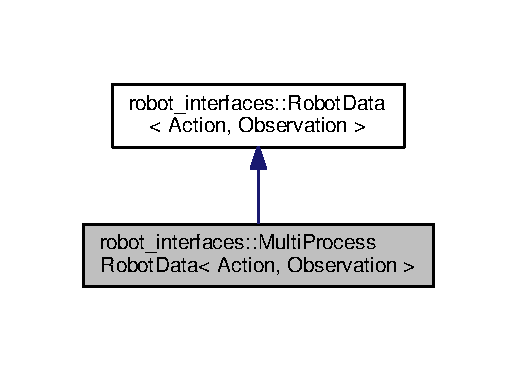
\includegraphics[width=248pt]{classrobot__interfaces_1_1MultiProcessRobotData__inherit__graph}
\end{center}
\end{figure}


Collaboration diagram for robot\+\_\+interfaces\+:\+:Multi\+Process\+Robot\+Data$<$ Action, Observation $>$\+:
\nopagebreak
\begin{figure}[H]
\begin{center}
\leavevmode
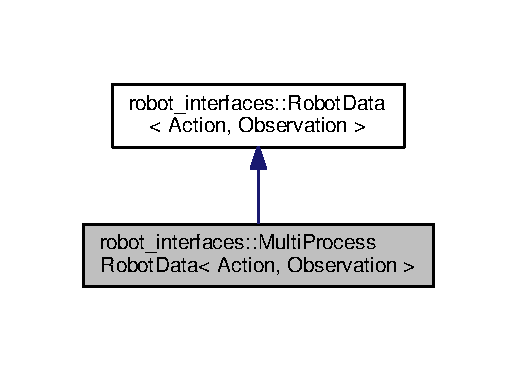
\includegraphics[width=248pt]{classrobot__interfaces_1_1MultiProcessRobotData__coll__graph}
\end{center}
\end{figure}
\subsection*{Public Member Functions}
\begin{DoxyCompactItemize}
\item 
\hyperlink{classrobot__interfaces_1_1MultiProcessRobotData_a27bb5ee187ceacb386d89c828481b057}{Multi\+Process\+Robot\+Data} (const std\+::string \&shared\+\_\+memory\+\_\+id\+\_\+prefix, bool is\+\_\+master, size\+\_\+t history\+\_\+length=1000)
\begin{DoxyCompactList}\small\item\em Construct the time series for the robot data. \end{DoxyCompactList}\end{DoxyCompactItemize}
\subsection*{Additional Inherited Members}


\subsection{Detailed Description}
\subsubsection*{template$<$typename Action, typename Observation$>$\\*
class robot\+\_\+interfaces\+::\+Multi\+Process\+Robot\+Data$<$ Action, Observation $>$}

\hyperlink{classrobot__interfaces_1_1RobotData}{Robot\+Data} instance using multi process time series. 

Use this class if modules accessing the data are running in separate processes. When all modules run as threads in the same process, this class can be used as well, however, \hyperlink{classrobot__interfaces_1_1SingleProcessRobotData}{Single\+Process\+Robot\+Data} might be more efficient in that case.

Contains all the input and output data of the robot. This means the
\begin{DoxyItemize}
\item {\ttfamily desired\+\_\+action} which was requested by the robot user
\item {\ttfamily applied\+\_\+action} which was actually applied and may not be and may not be identical to desired\+\_\+action for safety reasons
\item {\ttfamily observation} made by the robot
\item {\ttfamily status} which keeps track of timing issues and errors.
\end{DoxyItemize}

See this graph to understand how they relate to each other precisely in terms of time\+:

\begin{DoxyVerb}|------ t = 0 ------|------ t = 1 ------|
|----- action0 -----|----- action1 -----|
o                   o                   o
b                   b                   b
s                   s                   s
0                   1                   2
\end{DoxyVerb}



\begin{DoxyTemplParams}{Template Parameters}
{\em \hyperlink{classAction}{Action}} & Type of the actions. \\
\hline
{\em \hyperlink{classObservation}{Observation}} & Type of the observations. \\
\hline
\end{DoxyTemplParams}
\begin{DoxySeeAlso}{See also}
\hyperlink{classrobot__interfaces_1_1SingleProcessRobotData}{Single\+Process\+Robot\+Data} 
\end{DoxySeeAlso}
\begin{Desc}
\item[Examples\+: ]\par
\hyperlink{demo_multiprocess_backend_8cpp-example}{demo\+\_\+multiprocess\+\_\+backend.\+cpp}, and \hyperlink{demo_multiprocess_frontend_8cpp-example}{demo\+\_\+multiprocess\+\_\+frontend.\+cpp}.\end{Desc}


\subsection{Constructor \& Destructor Documentation}
\index{robot\+\_\+interfaces\+::\+Multi\+Process\+Robot\+Data@{robot\+\_\+interfaces\+::\+Multi\+Process\+Robot\+Data}!Multi\+Process\+Robot\+Data@{Multi\+Process\+Robot\+Data}}
\index{Multi\+Process\+Robot\+Data@{Multi\+Process\+Robot\+Data}!robot\+\_\+interfaces\+::\+Multi\+Process\+Robot\+Data@{robot\+\_\+interfaces\+::\+Multi\+Process\+Robot\+Data}}
\subsubsection[{\texorpdfstring{Multi\+Process\+Robot\+Data(const std\+::string \&shared\+\_\+memory\+\_\+id\+\_\+prefix, bool is\+\_\+master, size\+\_\+t history\+\_\+length=1000)}{MultiProcessRobotData(const std::string &shared_memory_id_prefix, bool is_master, size_t history_length=1000)}}]{\setlength{\rightskip}{0pt plus 5cm}template$<$typename Action , typename Observation $>$ {\bf robot\+\_\+interfaces\+::\+Multi\+Process\+Robot\+Data}$<$ {\bf Action}, {\bf Observation} $>$\+::{\bf Multi\+Process\+Robot\+Data} (
\begin{DoxyParamCaption}
\item[{const std\+::string \&}]{shared\+\_\+memory\+\_\+id\+\_\+prefix, }
\item[{bool}]{is\+\_\+master, }
\item[{size\+\_\+t}]{history\+\_\+length = {\ttfamily 1000}}
\end{DoxyParamCaption}
)\hspace{0.3cm}{\ttfamily [inline]}}\hypertarget{classrobot__interfaces_1_1MultiProcessRobotData_a27bb5ee187ceacb386d89c828481b057}{}\label{classrobot__interfaces_1_1MultiProcessRobotData_a27bb5ee187ceacb386d89c828481b057}


Construct the time series for the robot data. 


\begin{DoxyParams}{Parameters}
{\em shared\+\_\+memory\+\_\+id\+\_\+prefix} & Prefix for the shared memory I\+Ds. Since each time series needs its own memory ID, the given value is used as prefix and unique suffixes are appended. Make sure to use a prefix that cannot lead to name collisions on your system. \\
\hline
{\em is\+\_\+master} & If set to true, this instance will clear the shared memory on construction and destruction. Only once instance should act as master in a multi-\/process setup. \\
\hline
{\em history\+\_\+length} & History length of the time series. \\
\hline
\end{DoxyParams}


The documentation for this class was generated from the following file\+:\begin{DoxyCompactItemize}
\item 
include/robot\+\_\+interfaces/\hyperlink{robot__data_8hpp}{robot\+\_\+data.\+hpp}\end{DoxyCompactItemize}

\hypertarget{structrobot__interfaces_1_1NJointRobotFunctions}{}\section{robot\+\_\+interfaces\+:\+:N\+Joint\+Robot\+Functions$<$ N\+\_\+\+J\+O\+I\+N\+TS $>$ Struct Template Reference}
\label{structrobot__interfaces_1_1NJointRobotFunctions}\index{robot\+\_\+interfaces\+::\+N\+Joint\+Robot\+Functions$<$ N\+\_\+\+J\+O\+I\+N\+T\+S $>$@{robot\+\_\+interfaces\+::\+N\+Joint\+Robot\+Functions$<$ N\+\_\+\+J\+O\+I\+N\+T\+S $>$}}


Collection of functions for a generic N-\/joint B\+L\+MC robot.  




{\ttfamily \#include $<$n\+\_\+joint\+\_\+robot\+\_\+functions.\+hpp$>$}

\subsection*{Public Types}
\begin{DoxyCompactItemize}
\item 
using {\bfseries Types} = \hyperlink{structrobot__interfaces_1_1NJointRobotTypes}{N\+Joint\+Robot\+Types}$<$ N\+\_\+\+J\+O\+I\+N\+TS $>$\hypertarget{structrobot__interfaces_1_1NJointRobotFunctions_a7ace341ed7d3f1302264384b411c63e8}{}\label{structrobot__interfaces_1_1NJointRobotFunctions_a7ace341ed7d3f1302264384b411c63e8}

\end{DoxyCompactItemize}
\subsection*{Static Public Member Functions}
\begin{DoxyCompactItemize}
\item 
static \hyperlink{structrobot__interfaces_1_1NJointRobotTypes_1_1Action}{Types\+::\+Action} \hyperlink{structrobot__interfaces_1_1NJointRobotFunctions_a25eefa719e07b4499fe3fd6462d866df}{process\+\_\+desired\+\_\+action} (const typename \hyperlink{structrobot__interfaces_1_1NJointRobotTypes_1_1Action}{Types\+::\+Action} \&desired\+\_\+action, const typename \hyperlink{structrobot__interfaces_1_1NJointRobotTypes_1_1Observation}{Types\+::\+Observation} \&latest\+\_\+observation, const double max\+\_\+torque\+\_\+\+Nm, const typename Types\+::\+Vector \&safety\+\_\+kd, const typename Types\+::\+Vector \&default\+\_\+position\+\_\+control\+\_\+kp, const typename Types\+::\+Vector \&default\+\_\+position\+\_\+control\+\_\+kd)
\begin{DoxyCompactList}\small\item\em Process the desired action provided by the user. \end{DoxyCompactList}\end{DoxyCompactItemize}


\subsection{Detailed Description}
\subsubsection*{template$<$size\+\_\+t N\+\_\+\+J\+O\+I\+N\+TS$>$\\*
struct robot\+\_\+interfaces\+::\+N\+Joint\+Robot\+Functions$<$ N\+\_\+\+J\+O\+I\+N\+T\+S $>$}

Collection of functions for a generic N-\/joint B\+L\+MC robot. 

Defines all the types needed to set up an interface to a generic N-\/joint B\+L\+MC robot that expects as \hyperlink{classAction}{Action} a simple vector of N torque commands and provides N observations containing measured joint angle, velocity and torque.

Defines some generic functions that can be used by all robots that are based on the {\ttfamily \hyperlink{structrobot__interfaces_1_1NJointRobotTypes}{N\+Joint\+Robot\+Types}}.


\begin{DoxyTemplParams}{Template Parameters}
{\em N\+\_\+\+J\+O\+I\+N\+TS} & Number of joints the robot has. \\
\hline
\end{DoxyTemplParams}


\subsection{Member Function Documentation}
\index{robot\+\_\+interfaces\+::\+N\+Joint\+Robot\+Functions@{robot\+\_\+interfaces\+::\+N\+Joint\+Robot\+Functions}!process\+\_\+desired\+\_\+action@{process\+\_\+desired\+\_\+action}}
\index{process\+\_\+desired\+\_\+action@{process\+\_\+desired\+\_\+action}!robot\+\_\+interfaces\+::\+N\+Joint\+Robot\+Functions@{robot\+\_\+interfaces\+::\+N\+Joint\+Robot\+Functions}}
\subsubsection[{\texorpdfstring{process\+\_\+desired\+\_\+action(const typename Types\+::\+Action \&desired\+\_\+action, const typename Types\+::\+Observation \&latest\+\_\+observation, const double max\+\_\+torque\+\_\+\+Nm, const typename Types\+::\+Vector \&safety\+\_\+kd, const typename Types\+::\+Vector \&default\+\_\+position\+\_\+control\+\_\+kp, const typename Types\+::\+Vector \&default\+\_\+position\+\_\+control\+\_\+kd)}{process_desired_action(const typename Types::Action &desired_action, const typename Types::Observation &latest_observation, const double max_torque_Nm, const typename Types::Vector &safety_kd, const typename Types::Vector &default_position_control_kp, const typename Types::Vector &default_position_control_kd)}}]{\setlength{\rightskip}{0pt plus 5cm}template$<$size\+\_\+t N\+\_\+\+J\+O\+I\+N\+TS$>$ static {\bf Types\+::\+Action} {\bf robot\+\_\+interfaces\+::\+N\+Joint\+Robot\+Functions}$<$ N\+\_\+\+J\+O\+I\+N\+TS $>$\+::process\+\_\+desired\+\_\+action (
\begin{DoxyParamCaption}
\item[{const typename {\bf Types\+::\+Action} \&}]{desired\+\_\+action, }
\item[{const typename {\bf Types\+::\+Observation} \&}]{latest\+\_\+observation, }
\item[{const double}]{max\+\_\+torque\+\_\+\+Nm, }
\item[{const typename Types\+::\+Vector \&}]{safety\+\_\+kd, }
\item[{const typename Types\+::\+Vector \&}]{default\+\_\+position\+\_\+control\+\_\+kp, }
\item[{const typename Types\+::\+Vector \&}]{default\+\_\+position\+\_\+control\+\_\+kd}
\end{DoxyParamCaption}
)\hspace{0.3cm}{\ttfamily [inline]}, {\ttfamily [static]}}\hypertarget{structrobot__interfaces_1_1NJointRobotFunctions_a25eefa719e07b4499fe3fd6462d866df}{}\label{structrobot__interfaces_1_1NJointRobotFunctions_a25eefa719e07b4499fe3fd6462d866df}


Process the desired action provided by the user. 

Takes the desired action from the user and does the following processing\+:

\subsubsection*{1. Run the position controller in case a target position is set.}

If the target position is set to a value unequal to NaN for any joint, a PD position controller is executed for this joint and the resulting torque command is added to the torque command in the action.

If the P-\/ and/or D-\/gains are set to a non-\/\+NaN value in the action, they are used for the control. Na\+N-\/values are replaced with the default gains.

\subsubsection*{2. Apply safety checks.}


\begin{DoxyItemize}
\item Limit the torque to the allowed maximum value.
\item Dampen velocity using the given safety\+\_\+kd gains. Damping us done joint-\/wise using this equation\+: \begin{DoxyVerb}torque_damped = torque_desired - safety_kd * current_velocity
\end{DoxyVerb}

\end{DoxyItemize}

The resulting action with modifications of all steps is returned.


\begin{DoxyParams}{Parameters}
{\em desired\+\_\+action} & Desired action given by the user. \\
\hline
{\em latest\+\_\+observation} & Latest observation from the robot. \\
\hline
{\em max\+\_\+torque\+\_\+\+Nm} & Maximum allowed absolute torque. \\
\hline
{\em safety\+\_\+kd} & D-\/gain for velocity damping. \\
\hline
{\em default\+\_\+position\+\_\+control\+\_\+kp} & Default P-\/gain for position control. \\
\hline
{\em default\+\_\+position\+\_\+control\+\_\+kd} & Default D-\/gain for position control.\\
\hline
\end{DoxyParams}
\begin{DoxyReturn}{Returns}
Resulting action after applying all the processing. 
\end{DoxyReturn}


The documentation for this struct was generated from the following file\+:\begin{DoxyCompactItemize}
\item 
include/robot\+\_\+interfaces/n\+\_\+joint\+\_\+robot\+\_\+functions.\+hpp\end{DoxyCompactItemize}

\hypertarget{structrobot__interfaces_1_1NJointRobotTypes}{}\section{robot\+\_\+interfaces\+:\+:N\+Joint\+Robot\+Types$<$ N $>$ Struct Template Reference}
\label{structrobot__interfaces_1_1NJointRobotTypes}\index{robot\+\_\+interfaces\+::\+N\+Joint\+Robot\+Types$<$ N $>$@{robot\+\_\+interfaces\+::\+N\+Joint\+Robot\+Types$<$ N $>$}}


Collection of types for a generic N-\/joint B\+L\+MC robot.  




{\ttfamily \#include $<$n\+\_\+joint\+\_\+robot\+\_\+types.\+hpp$>$}

\subsection*{Classes}
\begin{DoxyCompactItemize}
\item 
struct \hyperlink{structrobot__interfaces_1_1NJointRobotTypes_1_1Action}{Action}
\item 
struct \hyperlink{structrobot__interfaces_1_1NJointRobotTypes_1_1Observation}{Observation}
\end{DoxyCompactItemize}
\subsection*{Public Types}
\begin{DoxyCompactItemize}
\item 
typedef Eigen\+::\+Matrix$<$ double, N, 1 $>$ {\bfseries Vector}\hypertarget{structrobot__interfaces_1_1NJointRobotTypes_a2c8ab754133625e175456e0f81753eb3}{}\label{structrobot__interfaces_1_1NJointRobotTypes_a2c8ab754133625e175456e0f81753eb3}

\item 
typedef \hyperlink{classrobot__interfaces_1_1RobotBackend}{Robot\+Backend}$<$ \hyperlink{structrobot__interfaces_1_1NJointRobotTypes_1_1Action}{Action}, \hyperlink{structrobot__interfaces_1_1NJointRobotTypes_1_1Observation}{Observation} $>$ {\bfseries Backend}\hypertarget{structrobot__interfaces_1_1NJointRobotTypes_aee4f8ae91b6d7b31852c4e5ad82635ca}{}\label{structrobot__interfaces_1_1NJointRobotTypes_aee4f8ae91b6d7b31852c4e5ad82635ca}

\item 
typedef std\+::shared\+\_\+ptr$<$ \hyperlink{classrobot__interfaces_1_1RobotBackend}{Backend} $>$ {\bfseries Backend\+Ptr}\hypertarget{structrobot__interfaces_1_1NJointRobotTypes_af7a865b80531a7b8e36368ad8bd8ce7e}{}\label{structrobot__interfaces_1_1NJointRobotTypes_af7a865b80531a7b8e36368ad8bd8ce7e}

\item 
typedef \hyperlink{classrobot__interfaces_1_1RobotData}{Robot\+Data}$<$ \hyperlink{structrobot__interfaces_1_1NJointRobotTypes_1_1Action}{Action}, \hyperlink{structrobot__interfaces_1_1NJointRobotTypes_1_1Observation}{Observation} $>$ {\bfseries Base\+Data}\hypertarget{structrobot__interfaces_1_1NJointRobotTypes_a87d6d758d4b569e795eb977cd738d29a}{}\label{structrobot__interfaces_1_1NJointRobotTypes_a87d6d758d4b569e795eb977cd738d29a}

\item 
typedef std\+::shared\+\_\+ptr$<$ \hyperlink{classrobot__interfaces_1_1RobotData}{Base\+Data} $>$ {\bfseries Base\+Data\+Ptr}\hypertarget{structrobot__interfaces_1_1NJointRobotTypes_a080b4a9042dd2c795f2af486fc33d9dc}{}\label{structrobot__interfaces_1_1NJointRobotTypes_a080b4a9042dd2c795f2af486fc33d9dc}

\item 
typedef \hyperlink{classrobot__interfaces_1_1SingleProcessRobotData}{Single\+Process\+Robot\+Data}$<$ \hyperlink{structrobot__interfaces_1_1NJointRobotTypes_1_1Action}{Action}, \hyperlink{structrobot__interfaces_1_1NJointRobotTypes_1_1Observation}{Observation} $>$ {\bfseries Single\+Process\+Data}\hypertarget{structrobot__interfaces_1_1NJointRobotTypes_a5cd0e28d0542c4949f0780082e35a48c}{}\label{structrobot__interfaces_1_1NJointRobotTypes_a5cd0e28d0542c4949f0780082e35a48c}

\item 
typedef std\+::shared\+\_\+ptr$<$ \hyperlink{classrobot__interfaces_1_1SingleProcessRobotData}{Single\+Process\+Data} $>$ {\bfseries Single\+Process\+Data\+Ptr}\hypertarget{structrobot__interfaces_1_1NJointRobotTypes_a98ad0ce92d0a999ef0345225d198f790}{}\label{structrobot__interfaces_1_1NJointRobotTypes_a98ad0ce92d0a999ef0345225d198f790}

\item 
typedef \hyperlink{classrobot__interfaces_1_1MultiProcessRobotData}{Multi\+Process\+Robot\+Data}$<$ \hyperlink{structrobot__interfaces_1_1NJointRobotTypes_1_1Action}{Action}, \hyperlink{structrobot__interfaces_1_1NJointRobotTypes_1_1Observation}{Observation} $>$ {\bfseries Multi\+Process\+Data}\hypertarget{structrobot__interfaces_1_1NJointRobotTypes_a4dff725737b41b840db7b7af6c64718f}{}\label{structrobot__interfaces_1_1NJointRobotTypes_a4dff725737b41b840db7b7af6c64718f}

\item 
typedef std\+::shared\+\_\+ptr$<$ \hyperlink{classrobot__interfaces_1_1MultiProcessRobotData}{Multi\+Process\+Data} $>$ {\bfseries Multi\+Process\+Data\+Ptr}\hypertarget{structrobot__interfaces_1_1NJointRobotTypes_a231d94c36fcddaa6e3fefd54e8fb8d82}{}\label{structrobot__interfaces_1_1NJointRobotTypes_a231d94c36fcddaa6e3fefd54e8fb8d82}

\item 
typedef \hyperlink{classrobot__interfaces_1_1RobotFrontend}{Robot\+Frontend}$<$ \hyperlink{structrobot__interfaces_1_1NJointRobotTypes_1_1Action}{Action}, \hyperlink{structrobot__interfaces_1_1NJointRobotTypes_1_1Observation}{Observation} $>$ {\bfseries Frontend}\hypertarget{structrobot__interfaces_1_1NJointRobotTypes_acfa2fab5ec37d832d80c9147e28903ec}{}\label{structrobot__interfaces_1_1NJointRobotTypes_acfa2fab5ec37d832d80c9147e28903ec}

\item 
typedef std\+::shared\+\_\+ptr$<$ \hyperlink{classrobot__interfaces_1_1RobotFrontend}{Frontend} $>$ {\bfseries Frontend\+Ptr}\hypertarget{structrobot__interfaces_1_1NJointRobotTypes_ab97eb0bbf6e63868dd1c215249742b04}{}\label{structrobot__interfaces_1_1NJointRobotTypes_ab97eb0bbf6e63868dd1c215249742b04}

\item 
typedef \hyperlink{classrobot__interfaces_1_1RobotLogger}{Robot\+Logger}$<$ \hyperlink{structrobot__interfaces_1_1NJointRobotTypes_1_1Action}{Action}, \hyperlink{structrobot__interfaces_1_1NJointRobotTypes_1_1Observation}{Observation} $>$ {\bfseries Logger}\hypertarget{structrobot__interfaces_1_1NJointRobotTypes_a3e170adc934171b70773e9f96b3d3c55}{}\label{structrobot__interfaces_1_1NJointRobotTypes_a3e170adc934171b70773e9f96b3d3c55}

\end{DoxyCompactItemize}


\subsection{Detailed Description}
\subsubsection*{template$<$size\+\_\+t N$>$\\*
struct robot\+\_\+interfaces\+::\+N\+Joint\+Robot\+Types$<$ N $>$}

Collection of types for a generic N-\/joint B\+L\+MC robot. 

Defines all the types needed to set up an interface to a generic N-\/joint B\+L\+MC robot that expects as \hyperlink{structrobot__interfaces_1_1NJointRobotTypes_1_1Action}{Action} a simple vector of N torque commands and provides N observations containing measured joint angle, velocity and torque.


\begin{DoxyTemplParams}{Template Parameters}
{\em N} & Number of joints \\
\hline
\end{DoxyTemplParams}


The documentation for this struct was generated from the following file\+:\begin{DoxyCompactItemize}
\item 
include/robot\+\_\+interfaces/n\+\_\+joint\+\_\+robot\+\_\+types.\+hpp\end{DoxyCompactItemize}

\hypertarget{classObservation}{}\section{Observation Class Reference}
\label{classObservation}\index{Observation@{Observation}}
\subsection*{Public Member Functions}
\begin{DoxyCompactItemize}
\item 
void {\bfseries print} (bool backline)\hypertarget{classObservation_acbc2da8c3b6b8c80feef13ceb203be65}{}\label{classObservation_acbc2da8c3b6b8c80feef13ceb203be65}

\end{DoxyCompactItemize}
\subsection*{Public Attributes}
\begin{DoxyCompactItemize}
\item 
int {\bfseries values} \mbox{[}2\mbox{]}\hypertarget{classObservation_a87baf44e3dbe1c7c43df49a9311d2c05}{}\label{classObservation_a87baf44e3dbe1c7c43df49a9311d2c05}

\end{DoxyCompactItemize}


\subsection{Detailed Description}
\begin{Desc}
\item[Examples\+: ]\par
\hyperlink{demo_8cpp-example}{demo.\+cpp}.\end{Desc}


The documentation for this class was generated from the following file\+:\begin{DoxyCompactItemize}
\item 
demos/\hyperlink{demo_8cpp}{demo.\+cpp}\end{DoxyCompactItemize}

\hypertarget{classrobot__interfaces_1_1demo_1_1Observation}{}\section{robot\+\_\+interfaces\+:\+:demo\+:\+:Observation Class Reference}
\label{classrobot__interfaces_1_1demo_1_1Observation}\index{robot\+\_\+interfaces\+::demo\+::\+Observation@{robot\+\_\+interfaces\+::demo\+::\+Observation}}


Read from the robot by \hyperlink{classDriver}{Driver}.  




{\ttfamily \#include $<$types.\+hpp$>$}

\subsection*{Public Member Functions}
\begin{DoxyCompactItemize}
\item 
void {\bfseries print} (bool backline) const \hypertarget{classrobot__interfaces_1_1demo_1_1Observation_a59e12a89db80a6b76791e313bcbef8b3}{}\label{classrobot__interfaces_1_1demo_1_1Observation_a59e12a89db80a6b76791e313bcbef8b3}

\item 
{\footnotesize template$<$class Archive $>$ }\\void {\bfseries serialize} (Archive \&ar)\hypertarget{classrobot__interfaces_1_1demo_1_1Observation_adc50512a62b26a896da47f6f67dee44e}{}\label{classrobot__interfaces_1_1demo_1_1Observation_adc50512a62b26a896da47f6f67dee44e}

\end{DoxyCompactItemize}
\subsection*{Public Attributes}
\begin{DoxyCompactItemize}
\item 
int {\bfseries values} \mbox{[}2\mbox{]}\hypertarget{classrobot__interfaces_1_1demo_1_1Observation_a930664896eceed4f3ee0de6f0e29bea4}{}\label{classrobot__interfaces_1_1demo_1_1Observation_a930664896eceed4f3ee0de6f0e29bea4}

\end{DoxyCompactItemize}


\subsection{Detailed Description}
Read from the robot by \hyperlink{classDriver}{Driver}. 

An observation is the current position for each dof. \begin{Desc}
\item[Examples\+: ]\par
\hyperlink{demo_multiprocess_backend_8cpp-example}{demo\+\_\+multiprocess\+\_\+backend.\+cpp}, and \hyperlink{demo_multiprocess_frontend_8cpp-example}{demo\+\_\+multiprocess\+\_\+frontend.\+cpp}.\end{Desc}


The documentation for this class was generated from the following file\+:\begin{DoxyCompactItemize}
\item 
demos/\hyperlink{types_8hpp}{types.\+hpp}\end{DoxyCompactItemize}

\hypertarget{structrobot__interfaces_1_1NJointRobotTypes_1_1Observation}{}\section{robot\+\_\+interfaces\+:\+:N\+Joint\+Robot\+Types$<$ N $>$\+:\+:Observation Struct Reference}
\label{structrobot__interfaces_1_1NJointRobotTypes_1_1Observation}\index{robot\+\_\+interfaces\+::\+N\+Joint\+Robot\+Types$<$ N $>$\+::\+Observation@{robot\+\_\+interfaces\+::\+N\+Joint\+Robot\+Types$<$ N $>$\+::\+Observation}}


Inheritance diagram for robot\+\_\+interfaces\+:\+:N\+Joint\+Robot\+Types$<$ N $>$\+:\+:Observation\+:
\nopagebreak
\begin{figure}[H]
\begin{center}
\leavevmode
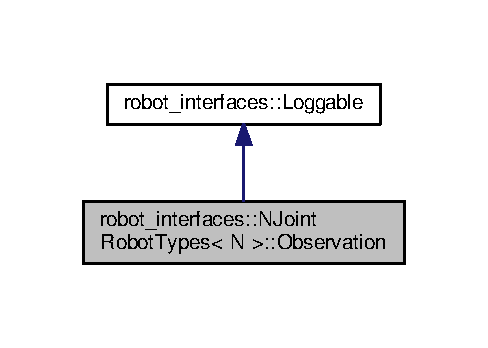
\includegraphics[width=234pt]{structrobot__interfaces_1_1NJointRobotTypes_1_1Observation__inherit__graph}
\end{center}
\end{figure}


Collaboration diagram for robot\+\_\+interfaces\+:\+:N\+Joint\+Robot\+Types$<$ N $>$\+:\+:Observation\+:
\nopagebreak
\begin{figure}[H]
\begin{center}
\leavevmode
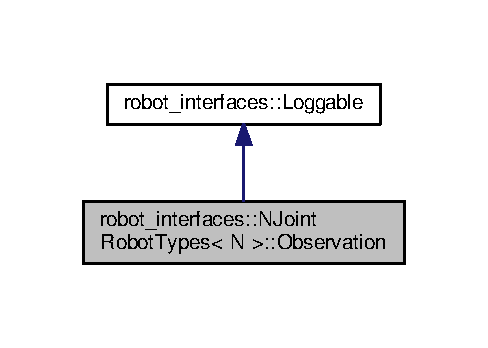
\includegraphics[width=234pt]{structrobot__interfaces_1_1NJointRobotTypes_1_1Observation__coll__graph}
\end{center}
\end{figure}
\subsection*{Public Member Functions}
\begin{DoxyCompactItemize}
\item 
{\footnotesize template$<$class Archive $>$ }\\void {\bfseries serialize} (Archive \&archive)\hypertarget{structrobot__interfaces_1_1NJointRobotTypes_1_1Observation_a9a94b6938b2dc8c71468d11a721330db}{}\label{structrobot__interfaces_1_1NJointRobotTypes_1_1Observation_a9a94b6938b2dc8c71468d11a721330db}

\item 
std\+::vector$<$ std\+::string $>$ {\bfseries get\+\_\+name} () override\hypertarget{structrobot__interfaces_1_1NJointRobotTypes_1_1Observation_a9eda538dfcaf22f36a879e0b6b11e856}{}\label{structrobot__interfaces_1_1NJointRobotTypes_1_1Observation_a9eda538dfcaf22f36a879e0b6b11e856}

\item 
std\+::vector$<$ std\+::vector$<$ double $>$ $>$ {\bfseries get\+\_\+data} () override\hypertarget{structrobot__interfaces_1_1NJointRobotTypes_1_1Observation_a874a72549cdd211ee60390e7df46a4bc}{}\label{structrobot__interfaces_1_1NJointRobotTypes_1_1Observation_a874a72549cdd211ee60390e7df46a4bc}

\end{DoxyCompactItemize}
\subsection*{Public Attributes}
\begin{DoxyCompactItemize}
\item 
Vector {\bfseries position}\hypertarget{structrobot__interfaces_1_1NJointRobotTypes_1_1Observation_a69885da4fb153f7157e1573d6347a3d5}{}\label{structrobot__interfaces_1_1NJointRobotTypes_1_1Observation_a69885da4fb153f7157e1573d6347a3d5}

\item 
Vector {\bfseries velocity}\hypertarget{structrobot__interfaces_1_1NJointRobotTypes_1_1Observation_a177d11f7a5f097b8a2d6959619812890}{}\label{structrobot__interfaces_1_1NJointRobotTypes_1_1Observation_a177d11f7a5f097b8a2d6959619812890}

\item 
Vector {\bfseries torque}\hypertarget{structrobot__interfaces_1_1NJointRobotTypes_1_1Observation_a01a13c04af01d13e0eedde954d9eb84d}{}\label{structrobot__interfaces_1_1NJointRobotTypes_1_1Observation_a01a13c04af01d13e0eedde954d9eb84d}

\end{DoxyCompactItemize}


The documentation for this struct was generated from the following file\+:\begin{DoxyCompactItemize}
\item 
include/robot\+\_\+interfaces/n\+\_\+joint\+\_\+robot\+\_\+types.\+hpp\end{DoxyCompactItemize}

\hypertarget{classrobot__interfaces_1_1Robot}{}\section{robot\+\_\+interfaces\+:\+:Robot$<$ Action, Observation, Driver, Data $>$ Class Template Reference}
\label{classrobot__interfaces_1_1Robot}\index{robot\+\_\+interfaces\+::\+Robot$<$ Action, Observation, Driver, Data $>$@{robot\+\_\+interfaces\+::\+Robot$<$ Action, Observation, Driver, Data $>$}}


\hyperlink{classrobot__interfaces_1_1RobotFrontend}{Robot\+Frontend} that construct and encapsulates its related \hyperlink{classrobot__interfaces_1_1RobotBackend}{Robot\+Backend}.  




{\ttfamily \#include $<$robot.\+hpp$>$}



Inheritance diagram for robot\+\_\+interfaces\+:\+:Robot$<$ Action, Observation, Driver, Data $>$\+:
\nopagebreak
\begin{figure}[H]
\begin{center}
\leavevmode
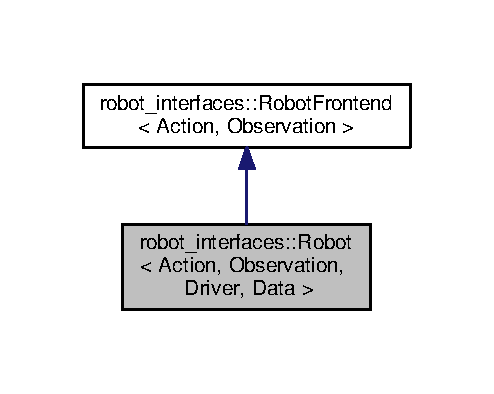
\includegraphics[width=237pt]{classrobot__interfaces_1_1Robot__inherit__graph}
\end{center}
\end{figure}


Collaboration diagram for robot\+\_\+interfaces\+:\+:Robot$<$ Action, Observation, Driver, Data $>$\+:
\nopagebreak
\begin{figure}[H]
\begin{center}
\leavevmode
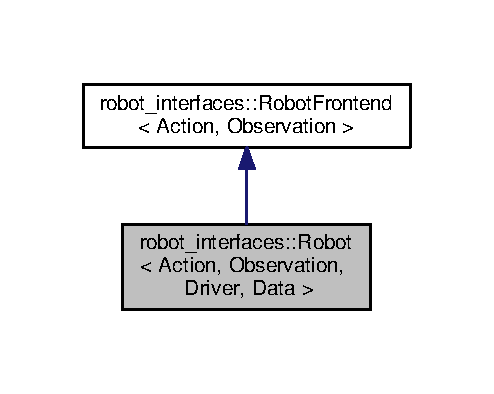
\includegraphics[width=237pt]{classrobot__interfaces_1_1Robot__coll__graph}
\end{center}
\end{figure}
\subsection*{Public Member Functions}
\begin{DoxyCompactItemize}
\item 
{\footnotesize template$<$typename... Args$>$ }\\\hyperlink{classrobot__interfaces_1_1Robot_a98609b8d6807e4407ab8d735a2dd412c}{Robot} (double max\+\_\+action\+\_\+duration\+\_\+s, double max\+\_\+inter\+\_\+action\+\_\+duration\+\_\+s, Args...\+args)
\item 
void \hyperlink{classrobot__interfaces_1_1Robot_af2d47a88a06f94e90bc0145ba1171cd0}{initialize} ()\hypertarget{classrobot__interfaces_1_1Robot_af2d47a88a06f94e90bc0145ba1171cd0}{}\label{classrobot__interfaces_1_1Robot_af2d47a88a06f94e90bc0145ba1171cd0}

\begin{DoxyCompactList}\small\item\em initialize the backend \end{DoxyCompactList}\item 
const Data \& \hyperlink{classrobot__interfaces_1_1Robot_a0f6854c5fe090ac0d675e0bf74afc953}{get\+\_\+data} () const \hypertarget{classrobot__interfaces_1_1Robot_a0f6854c5fe090ac0d675e0bf74afc953}{}\label{classrobot__interfaces_1_1Robot_a0f6854c5fe090ac0d675e0bf74afc953}

\begin{DoxyCompactList}\small\item\em return the data shared by the frontend and the backend. \end{DoxyCompactList}\end{DoxyCompactItemize}
\subsection*{Private Types}
\begin{DoxyCompactItemize}
\item 
typedef std\+::shared\+\_\+ptr$<$ Data $>$ {\bfseries Data\+Ptr}\hypertarget{classrobot__interfaces_1_1Robot_aae6cdfcef2853a056a6f7d7d2356b7df}{}\label{classrobot__interfaces_1_1Robot_aae6cdfcef2853a056a6f7d7d2356b7df}

\item 
typedef std\+::shared\+\_\+ptr$<$ \hyperlink{classDriver}{Driver} $>$ {\bfseries Robot\+Driver\+Ptr}\hypertarget{classrobot__interfaces_1_1Robot_a8aa32d96551cdd9234288203b1790f6d}{}\label{classrobot__interfaces_1_1Robot_a8aa32d96551cdd9234288203b1790f6d}

\end{DoxyCompactItemize}
\subsection*{Private Attributes}
\begin{DoxyCompactItemize}
\item 
Robot\+Driver\+Ptr {\bfseries driver\+\_\+ptr\+\_\+}\hypertarget{classrobot__interfaces_1_1Robot_add04574720fb6d4ecc9fd74678b3627e}{}\label{classrobot__interfaces_1_1Robot_add04574720fb6d4ecc9fd74678b3627e}

\item 
\hyperlink{classrobot__interfaces_1_1RobotBackend}{Robot\+Backend}$<$ \hyperlink{classAction}{Action}, \hyperlink{classObservation}{Observation} $>$ {\bfseries backend\+\_\+}\hypertarget{classrobot__interfaces_1_1Robot_abefd57cd42aad6c21b3db990d4488db4}{}\label{classrobot__interfaces_1_1Robot_abefd57cd42aad6c21b3db990d4488db4}

\end{DoxyCompactItemize}
\subsection*{Additional Inherited Members}


\subsection{Detailed Description}
\subsubsection*{template$<$typename Action, typename Observation, typename Driver, typename Data = Single\+Process\+Robot\+Data$<$\+Action, Observation$>$$>$\\*
class robot\+\_\+interfaces\+::\+Robot$<$ Action, Observation, Driver, Data $>$}

\hyperlink{classrobot__interfaces_1_1RobotFrontend}{Robot\+Frontend} that construct and encapsulates its related \hyperlink{classrobot__interfaces_1_1RobotBackend}{Robot\+Backend}. 

It also construct and starts the robot driver. \begin{Desc}
\item[Examples\+: ]\par
\hyperlink{demo_8cpp-example}{demo.\+cpp}.\end{Desc}


\subsection{Constructor \& Destructor Documentation}
\index{robot\+\_\+interfaces\+::\+Robot@{robot\+\_\+interfaces\+::\+Robot}!Robot@{Robot}}
\index{Robot@{Robot}!robot\+\_\+interfaces\+::\+Robot@{robot\+\_\+interfaces\+::\+Robot}}
\subsubsection[{\texorpdfstring{Robot(double max\+\_\+action\+\_\+duration\+\_\+s, double max\+\_\+inter\+\_\+action\+\_\+duration\+\_\+s, Args...\+args)}{Robot(double max_action_duration_s, double max_inter_action_duration_s, Args...args)}}]{\setlength{\rightskip}{0pt plus 5cm}template$<$typename Action , typename Observation , typename Driver , typename Data  = Single\+Process\+Robot\+Data$<$\+Action, Observation$>$$>$ template$<$typename... Args$>$ {\bf robot\+\_\+interfaces\+::\+Robot}$<$ {\bf Action}, {\bf Observation}, {\bf Driver}, Data $>$\+::{\bf Robot} (
\begin{DoxyParamCaption}
\item[{double}]{max\+\_\+action\+\_\+duration\+\_\+s, }
\item[{double}]{max\+\_\+inter\+\_\+action\+\_\+duration\+\_\+s, }
\item[{Args...}]{args}
\end{DoxyParamCaption}
)\hspace{0.3cm}{\ttfamily [inline]}}\hypertarget{classrobot__interfaces_1_1Robot_a98609b8d6807e4407ab8d735a2dd412c}{}\label{classrobot__interfaces_1_1Robot_a98609b8d6807e4407ab8d735a2dd412c}

\begin{DoxyParams}{Parameters}
{\em max\+\_\+action\+\_\+duration\+\_\+s} & See \hyperlink{classrobot__interfaces_1_1MonitoredRobotDriver}{Monitored\+Robot\+Driver}. \\
\hline
{\em max\+\_\+inter\+\_\+action\+\_\+duration\+\_\+s} & See \hyperlink{classrobot__interfaces_1_1MonitoredRobotDriver}{Monitored\+Robot\+Driver}. \\
\hline
{\em args} & Arguments required to instantiate the driver by this constructor if not provided. \\
\hline
\end{DoxyParams}


The documentation for this class was generated from the following file\+:\begin{DoxyCompactItemize}
\item 
include/robot\+\_\+interfaces/robot.\+hpp\end{DoxyCompactItemize}

\hypertarget{classrobot__interfaces_1_1RobotBackend}{}\section{robot\+\_\+interfaces\+:\+:Robot\+Backend$<$ Action, Observation $>$ Class Template Reference}
\label{classrobot__interfaces_1_1RobotBackend}\index{robot\+\_\+interfaces\+::\+Robot\+Backend$<$ Action, Observation $>$@{robot\+\_\+interfaces\+::\+Robot\+Backend$<$ Action, Observation $>$}}


Communication link between \hyperlink{classrobot__interfaces_1_1RobotDriver}{Robot\+Driver} and \hyperlink{classrobot__interfaces_1_1RobotData}{Robot\+Data}.  




{\ttfamily \#include $<$robot\+\_\+backend.\+hpp$>$}

\subsection*{Public Member Functions}
\begin{DoxyCompactItemize}
\item 
\hyperlink{classrobot__interfaces_1_1RobotBackend_af454a09b5d269ed32b0ae2d35abdb833}{Robot\+Backend} (std\+::shared\+\_\+ptr$<$ \hyperlink{classrobot__interfaces_1_1RobotDriver}{Robot\+Driver}$<$ \hyperlink{classAction}{Action}, \hyperlink{classObservation}{Observation} $>$$>$ robot\+\_\+driver, std\+::shared\+\_\+ptr$<$ \hyperlink{classrobot__interfaces_1_1RobotData}{Robot\+Data}$<$ \hyperlink{classAction}{Action}, \hyperlink{classObservation}{Observation} $>$$>$ robot\+\_\+data, const bool real\+\_\+time\+\_\+mode=true, const double first\+\_\+action\+\_\+timeout=std\+::numeric\+\_\+limits$<$ double $>$\+::infinity(), const uint32\+\_\+t max\+\_\+number\+\_\+of\+\_\+actions=0)
\item 
uint32\+\_\+t {\bfseries get\+\_\+max\+\_\+action\+\_\+repetitions} ()\hypertarget{classrobot__interfaces_1_1RobotBackend_ae354dfd960d4fd0d2f9242dcfb4a701f}{}\label{classrobot__interfaces_1_1RobotBackend_ae354dfd960d4fd0d2f9242dcfb4a701f}

\item 
void \hyperlink{classrobot__interfaces_1_1RobotBackend_aad761d1e0ab7296a9632b9c4cc9c91db}{set\+\_\+max\+\_\+action\+\_\+repetitions} (const uint32\+\_\+t \&max\+\_\+action\+\_\+repetitions)
\begin{DoxyCompactList}\small\item\em Set how often an action is repeated if no new one is provided. \end{DoxyCompactList}\item 
void {\bfseries initialize} ()\hypertarget{classrobot__interfaces_1_1RobotBackend_a7e4eb9f5362b79c0c21b824e3b639ae6}{}\label{classrobot__interfaces_1_1RobotBackend_a7e4eb9f5362b79c0c21b824e3b639ae6}

\item 
void \hyperlink{classrobot__interfaces_1_1RobotBackend_a3da1748227b56acf7b745aff64023715}{request\+\_\+shutdown} ()
\begin{DoxyCompactList}\small\item\em Request shutdown of the backend loop. \end{DoxyCompactList}\item 
void \hyperlink{classrobot__interfaces_1_1RobotBackend_acc6fd15379502943f99b58bad9b0acf7}{wait\+\_\+until\+\_\+terminated} () const \hypertarget{classrobot__interfaces_1_1RobotBackend_acc6fd15379502943f99b58bad9b0acf7}{}\label{classrobot__interfaces_1_1RobotBackend_acc6fd15379502943f99b58bad9b0acf7}

\begin{DoxyCompactList}\small\item\em Wait until the backend loop terminates. \end{DoxyCompactList}\end{DoxyCompactItemize}
\subsection*{Private Member Functions}
\begin{DoxyCompactItemize}
\item 
bool {\bfseries has\+\_\+shutdown\+\_\+request} () const \hypertarget{classrobot__interfaces_1_1RobotBackend_afb4058468e7cc59dae5801eb5e369613}{}\label{classrobot__interfaces_1_1RobotBackend_afb4058468e7cc59dae5801eb5e369613}

\item 
void \hyperlink{classrobot__interfaces_1_1RobotBackend_a7cc66183743f277c41614a44fcc47b1a}{loop} ()
\begin{DoxyCompactList}\small\item\em Main loop. \end{DoxyCompactList}\end{DoxyCompactItemize}
\subsection*{Static Private Member Functions}
\begin{DoxyCompactItemize}
\item 
static void $\ast$ {\bfseries loop} (void $\ast$instance\+\_\+pointer)\hypertarget{classrobot__interfaces_1_1RobotBackend_a44f21ab5414ea7742e34a3cf3dfe0650}{}\label{classrobot__interfaces_1_1RobotBackend_a44f21ab5414ea7742e34a3cf3dfe0650}

\end{DoxyCompactItemize}
\subsection*{Private Attributes}
\begin{DoxyCompactItemize}
\item 
std\+::shared\+\_\+ptr$<$ \hyperlink{classrobot__interfaces_1_1RobotDriver}{Robot\+Driver}$<$ \hyperlink{classAction}{Action}, \hyperlink{classObservation}{Observation} $>$ $>$ {\bfseries robot\+\_\+driver\+\_\+}\hypertarget{classrobot__interfaces_1_1RobotBackend_a9c07b9b4a8c98b3f1b63d0754cbcb85b}{}\label{classrobot__interfaces_1_1RobotBackend_a9c07b9b4a8c98b3f1b63d0754cbcb85b}

\item 
std\+::shared\+\_\+ptr$<$ \hyperlink{classrobot__interfaces_1_1RobotData}{Robot\+Data}$<$ \hyperlink{classAction}{Action}, \hyperlink{classObservation}{Observation} $>$ $>$ {\bfseries robot\+\_\+data\+\_\+}\hypertarget{classrobot__interfaces_1_1RobotBackend_a4bb04e584d971d4d99a32ea8c5b0cd68}{}\label{classrobot__interfaces_1_1RobotBackend_a4bb04e584d971d4d99a32ea8c5b0cd68}

\item 
const bool \hyperlink{classrobot__interfaces_1_1RobotBackend_a81610183c52c9fe2088304bbd3b6f83f}{real\+\_\+time\+\_\+mode\+\_\+}
\begin{DoxyCompactList}\small\item\em Enable/disable real time mode. \end{DoxyCompactList}\item 
const double \hyperlink{classrobot__interfaces_1_1RobotBackend_a56f111a9e0663eedefbaf55de36f7cac}{first\+\_\+action\+\_\+timeout\+\_\+}
\begin{DoxyCompactList}\small\item\em Timeout for the first action to arrive. \end{DoxyCompactList}\item 
const uint32\+\_\+t \hyperlink{classrobot__interfaces_1_1RobotBackend_a7cac555549bff96a32da042a97919d47}{max\+\_\+number\+\_\+of\+\_\+actions\+\_\+}
\begin{DoxyCompactList}\small\item\em Maximum number of actions that are executed by the backend. \end{DoxyCompactList}\item 
std\+::atomic$<$ bool $>$ \hyperlink{classrobot__interfaces_1_1RobotBackend_abe24206dcf102b33f8ee472e287f485a}{is\+\_\+shutdown\+\_\+requested\+\_\+}
\begin{DoxyCompactList}\small\item\em Set to true when shutdown is requested. \end{DoxyCompactList}\item 
std\+::atomic$<$ bool $>$ \hyperlink{classrobot__interfaces_1_1RobotBackend_a0e91800b352b7b52f22820775b1d5e99}{loop\+\_\+is\+\_\+running\+\_\+}\hypertarget{classrobot__interfaces_1_1RobotBackend_a0e91800b352b7b52f22820775b1d5e99}{}\label{classrobot__interfaces_1_1RobotBackend_a0e91800b352b7b52f22820775b1d5e99}

\begin{DoxyCompactList}\small\item\em Indicates if the background loop is still running. \end{DoxyCompactList}\item 
uint32\+\_\+t \hyperlink{classrobot__interfaces_1_1RobotBackend_ae40ecdc44212f79f96d63a84f7b8a6e8}{max\+\_\+action\+\_\+repetitions\+\_\+}\hypertarget{classrobot__interfaces_1_1RobotBackend_ae40ecdc44212f79f96d63a84f7b8a6e8}{}\label{classrobot__interfaces_1_1RobotBackend_ae40ecdc44212f79f96d63a84f7b8a6e8}

\begin{DoxyCompactList}\small\item\em Number of times the previous action is repeated if no new one is provided. \end{DoxyCompactList}\item 
real\+\_\+time\+\_\+tools\+::\+Checkpoint\+Timer$<$ 6, false $>$ {\bfseries timer\+\_\+}\hypertarget{classrobot__interfaces_1_1RobotBackend_a69c9b7f07651484d1677121f72832482}{}\label{classrobot__interfaces_1_1RobotBackend_a69c9b7f07651484d1677121f72832482}

\item 
std\+::shared\+\_\+ptr$<$ real\+\_\+time\+\_\+tools\+::\+Real\+Time\+Thread $>$ {\bfseries thread\+\_\+}\hypertarget{classrobot__interfaces_1_1RobotBackend_afcf4f2443b7f3000cece9b0851284717}{}\label{classrobot__interfaces_1_1RobotBackend_afcf4f2443b7f3000cece9b0851284717}

\end{DoxyCompactItemize}


\subsection{Detailed Description}
\subsubsection*{template$<$typename Action, typename Observation$>$\\*
class robot\+\_\+interfaces\+::\+Robot\+Backend$<$ Action, Observation $>$}

Communication link between \hyperlink{classrobot__interfaces_1_1RobotDriver}{Robot\+Driver} and \hyperlink{classrobot__interfaces_1_1RobotData}{Robot\+Data}. 

At each time-\/step, it gets the observation from the \hyperlink{classrobot__interfaces_1_1RobotDriver}{Robot\+Driver} and writes it to \hyperlink{classrobot__interfaces_1_1RobotData}{Robot\+Data}, and it takes the desired\+\_\+action from \hyperlink{classrobot__interfaces_1_1RobotData}{Robot\+Data} and applies it on the \hyperlink{classrobot__interfaces_1_1RobotDriver}{Robot\+Driver}.


\begin{DoxyTemplParams}{Template Parameters}
{\em \hyperlink{classAction}{Action}} & \\
\hline
{\em \hyperlink{classObservation}{Observation}} & \\
\hline
\end{DoxyTemplParams}
\begin{Desc}
\item[Examples\+: ]\par
\hyperlink{demo_8cpp-example}{demo.\+cpp}, and \hyperlink{demo_multiprocess_backend_8cpp-example}{demo\+\_\+multiprocess\+\_\+backend.\+cpp}.\end{Desc}


\subsection{Constructor \& Destructor Documentation}
\index{robot\+\_\+interfaces\+::\+Robot\+Backend@{robot\+\_\+interfaces\+::\+Robot\+Backend}!Robot\+Backend@{Robot\+Backend}}
\index{Robot\+Backend@{Robot\+Backend}!robot\+\_\+interfaces\+::\+Robot\+Backend@{robot\+\_\+interfaces\+::\+Robot\+Backend}}
\subsubsection[{\texorpdfstring{Robot\+Backend(std\+::shared\+\_\+ptr$<$ Robot\+Driver$<$ Action, Observation $>$$>$ robot\+\_\+driver, std\+::shared\+\_\+ptr$<$ Robot\+Data$<$ Action, Observation $>$$>$ robot\+\_\+data, const bool real\+\_\+time\+\_\+mode=true, const double first\+\_\+action\+\_\+timeout=std\+::numeric\+\_\+limits$<$ double $>$\+::infinity(), const uint32\+\_\+t max\+\_\+number\+\_\+of\+\_\+actions=0)}{RobotBackend(std::shared_ptr< RobotDriver< Action, Observation >> robot_driver, std::shared_ptr< RobotData< Action, Observation >> robot_data, const bool real_time_mode=true, const double first_action_timeout=std::numeric_limits< double >::infinity(), const uint32_t max_number_of_actions=0)}}]{\setlength{\rightskip}{0pt plus 5cm}template$<$typename Action, typename Observation$>$ {\bf robot\+\_\+interfaces\+::\+Robot\+Backend}$<$ {\bf Action}, {\bf Observation} $>$\+::{\bf Robot\+Backend} (
\begin{DoxyParamCaption}
\item[{std\+::shared\+\_\+ptr$<$ {\bf Robot\+Driver}$<$ {\bf Action}, {\bf Observation} $>$$>$}]{robot\+\_\+driver, }
\item[{std\+::shared\+\_\+ptr$<$ {\bf Robot\+Data}$<$ {\bf Action}, {\bf Observation} $>$$>$}]{robot\+\_\+data, }
\item[{const bool}]{real\+\_\+time\+\_\+mode = {\ttfamily true}, }
\item[{const double}]{first\+\_\+action\+\_\+timeout = {\ttfamily std\+:\+:numeric\+\_\+limits$<$double$>$\+:\+:infinity()}, }
\item[{const uint32\+\_\+t}]{max\+\_\+number\+\_\+of\+\_\+actions = {\ttfamily 0}}
\end{DoxyParamCaption}
)\hspace{0.3cm}{\ttfamily [inline]}}\hypertarget{classrobot__interfaces_1_1RobotBackend_af454a09b5d269ed32b0ae2d35abdb833}{}\label{classrobot__interfaces_1_1RobotBackend_af454a09b5d269ed32b0ae2d35abdb833}

\begin{DoxyParams}{Parameters}
{\em robot\+\_\+driver} & \hyperlink{classDriver}{Driver} instance for the actual robot. \\
\hline
{\em robot\+\_\+data} & Data is send to/retrieved from here. \\
\hline
{\em real\+\_\+time\+\_\+mode} & Enable/disable real-\/time mode. In real-\/time mode, the backend will repeat previous actions if the new one is not provided in time or fail with an error if the allowed number of repetitions is exceeded. In non-\/real-\/time mode, it will simply block and wait until the action is provided. \\
\hline
{\em first\+\_\+action\+\_\+timeout} & See \hyperlink{classrobot__interfaces_1_1RobotBackend_a56f111a9e0663eedefbaf55de36f7cac}{Robot\+Backend\+::first\+\_\+action\+\_\+timeout\+\_\+}. \\
\hline
{\em max\+\_\+number\+\_\+of\+\_\+actions} & See \hyperlink{classrobot__interfaces_1_1RobotBackend_a7cac555549bff96a32da042a97919d47}{Robot\+Backend\+::max\+\_\+number\+\_\+of\+\_\+actions\+\_\+}. \\
\hline
\end{DoxyParams}


\subsection{Member Function Documentation}
\index{robot\+\_\+interfaces\+::\+Robot\+Backend@{robot\+\_\+interfaces\+::\+Robot\+Backend}!loop@{loop}}
\index{loop@{loop}!robot\+\_\+interfaces\+::\+Robot\+Backend@{robot\+\_\+interfaces\+::\+Robot\+Backend}}
\subsubsection[{\texorpdfstring{loop()}{loop()}}]{\setlength{\rightskip}{0pt plus 5cm}template$<$typename Action, typename Observation$>$ void {\bf robot\+\_\+interfaces\+::\+Robot\+Backend}$<$ {\bf Action}, {\bf Observation} $>$\+::loop (
\begin{DoxyParamCaption}
{}
\end{DoxyParamCaption}
)\hspace{0.3cm}{\ttfamily [inline]}, {\ttfamily [private]}}\hypertarget{classrobot__interfaces_1_1RobotBackend_a7cc66183743f277c41614a44fcc47b1a}{}\label{classrobot__interfaces_1_1RobotBackend_a7cc66183743f277c41614a44fcc47b1a}


Main loop. 

Iterate over robot\+\_\+data\+\_\+.\+desired\+\_\+action and apply these actions to the robot, and read the applied\+\_\+action and the observation from the robot and append them to the corresponding timeseries in robot\+\_\+data\+\_\+. \index{robot\+\_\+interfaces\+::\+Robot\+Backend@{robot\+\_\+interfaces\+::\+Robot\+Backend}!request\+\_\+shutdown@{request\+\_\+shutdown}}
\index{request\+\_\+shutdown@{request\+\_\+shutdown}!robot\+\_\+interfaces\+::\+Robot\+Backend@{robot\+\_\+interfaces\+::\+Robot\+Backend}}
\subsubsection[{\texorpdfstring{request\+\_\+shutdown()}{request_shutdown()}}]{\setlength{\rightskip}{0pt plus 5cm}template$<$typename Action, typename Observation$>$ void {\bf robot\+\_\+interfaces\+::\+Robot\+Backend}$<$ {\bf Action}, {\bf Observation} $>$\+::request\+\_\+shutdown (
\begin{DoxyParamCaption}
{}
\end{DoxyParamCaption}
)\hspace{0.3cm}{\ttfamily [inline]}}\hypertarget{classrobot__interfaces_1_1RobotBackend_a3da1748227b56acf7b745aff64023715}{}\label{classrobot__interfaces_1_1RobotBackend_a3da1748227b56acf7b745aff64023715}


Request shutdown of the backend loop. 

The loop may take some time to actually terminate after calling this function. Use \hyperlink{classrobot__interfaces_1_1RobotBackend_acc6fd15379502943f99b58bad9b0acf7}{wait\+\_\+until\+\_\+terminated()} to ensure it has really terminated. \index{robot\+\_\+interfaces\+::\+Robot\+Backend@{robot\+\_\+interfaces\+::\+Robot\+Backend}!set\+\_\+max\+\_\+action\+\_\+repetitions@{set\+\_\+max\+\_\+action\+\_\+repetitions}}
\index{set\+\_\+max\+\_\+action\+\_\+repetitions@{set\+\_\+max\+\_\+action\+\_\+repetitions}!robot\+\_\+interfaces\+::\+Robot\+Backend@{robot\+\_\+interfaces\+::\+Robot\+Backend}}
\subsubsection[{\texorpdfstring{set\+\_\+max\+\_\+action\+\_\+repetitions(const uint32\+\_\+t \&max\+\_\+action\+\_\+repetitions)}{set_max_action_repetitions(const uint32_t &max_action_repetitions)}}]{\setlength{\rightskip}{0pt plus 5cm}template$<$typename Action, typename Observation$>$ void {\bf robot\+\_\+interfaces\+::\+Robot\+Backend}$<$ {\bf Action}, {\bf Observation} $>$\+::set\+\_\+max\+\_\+action\+\_\+repetitions (
\begin{DoxyParamCaption}
\item[{const uint32\+\_\+t \&}]{max\+\_\+action\+\_\+repetitions}
\end{DoxyParamCaption}
)\hspace{0.3cm}{\ttfamily [inline]}}\hypertarget{classrobot__interfaces_1_1RobotBackend_aad761d1e0ab7296a9632b9c4cc9c91db}{}\label{classrobot__interfaces_1_1RobotBackend_aad761d1e0ab7296a9632b9c4cc9c91db}


Set how often an action is repeated if no new one is provided. 

If the next action is due to be executed but the user did not provide one yet (i.\+e. there is no new action in the robot data time series), the last action will be repeated by automatically adding it to the time series again.

Use this this method to specify how often the action shall be repeated (default is 0, i.\+e. no repetition at all). If this limit is exceeded, the robot will be shut down and the \hyperlink{classrobot__interfaces_1_1RobotBackend}{Robot\+Backend} stops.

{\bfseries Note\+:} This is ignored in non-\/real-\/time mode.


\begin{DoxyParams}{Parameters}
{\em max\+\_\+action\+\_\+repetitions} & \\
\hline
\end{DoxyParams}


\subsection{Member Data Documentation}
\index{robot\+\_\+interfaces\+::\+Robot\+Backend@{robot\+\_\+interfaces\+::\+Robot\+Backend}!first\+\_\+action\+\_\+timeout\+\_\+@{first\+\_\+action\+\_\+timeout\+\_\+}}
\index{first\+\_\+action\+\_\+timeout\+\_\+@{first\+\_\+action\+\_\+timeout\+\_\+}!robot\+\_\+interfaces\+::\+Robot\+Backend@{robot\+\_\+interfaces\+::\+Robot\+Backend}}
\subsubsection[{\texorpdfstring{first\+\_\+action\+\_\+timeout\+\_\+}{first_action_timeout_}}]{\setlength{\rightskip}{0pt plus 5cm}template$<$typename Action, typename Observation$>$ const double {\bf robot\+\_\+interfaces\+::\+Robot\+Backend}$<$ {\bf Action}, {\bf Observation} $>$\+::first\+\_\+action\+\_\+timeout\+\_\+\hspace{0.3cm}{\ttfamily [private]}}\hypertarget{classrobot__interfaces_1_1RobotBackend_a56f111a9e0663eedefbaf55de36f7cac}{}\label{classrobot__interfaces_1_1RobotBackend_a56f111a9e0663eedefbaf55de36f7cac}


Timeout for the first action to arrive. 

Timeout for the time between starting the backend loop and receiving the first action from the user. If exceeded, the backend shuts down. Set to infinity to disable the timeout. \index{robot\+\_\+interfaces\+::\+Robot\+Backend@{robot\+\_\+interfaces\+::\+Robot\+Backend}!is\+\_\+shutdown\+\_\+requested\+\_\+@{is\+\_\+shutdown\+\_\+requested\+\_\+}}
\index{is\+\_\+shutdown\+\_\+requested\+\_\+@{is\+\_\+shutdown\+\_\+requested\+\_\+}!robot\+\_\+interfaces\+::\+Robot\+Backend@{robot\+\_\+interfaces\+::\+Robot\+Backend}}
\subsubsection[{\texorpdfstring{is\+\_\+shutdown\+\_\+requested\+\_\+}{is_shutdown_requested_}}]{\setlength{\rightskip}{0pt plus 5cm}template$<$typename Action, typename Observation$>$ std\+::atomic$<$bool$>$ {\bf robot\+\_\+interfaces\+::\+Robot\+Backend}$<$ {\bf Action}, {\bf Observation} $>$\+::is\+\_\+shutdown\+\_\+requested\+\_\+\hspace{0.3cm}{\ttfamily [private]}}\hypertarget{classrobot__interfaces_1_1RobotBackend_abe24206dcf102b33f8ee472e287f485a}{}\label{classrobot__interfaces_1_1RobotBackend_abe24206dcf102b33f8ee472e287f485a}


Set to true when shutdown is requested. 

This is used to notify the background loop about requested shutdown, so it terminates itself. \index{robot\+\_\+interfaces\+::\+Robot\+Backend@{robot\+\_\+interfaces\+::\+Robot\+Backend}!max\+\_\+number\+\_\+of\+\_\+actions\+\_\+@{max\+\_\+number\+\_\+of\+\_\+actions\+\_\+}}
\index{max\+\_\+number\+\_\+of\+\_\+actions\+\_\+@{max\+\_\+number\+\_\+of\+\_\+actions\+\_\+}!robot\+\_\+interfaces\+::\+Robot\+Backend@{robot\+\_\+interfaces\+::\+Robot\+Backend}}
\subsubsection[{\texorpdfstring{max\+\_\+number\+\_\+of\+\_\+actions\+\_\+}{max_number_of_actions_}}]{\setlength{\rightskip}{0pt plus 5cm}template$<$typename Action, typename Observation$>$ const uint32\+\_\+t {\bf robot\+\_\+interfaces\+::\+Robot\+Backend}$<$ {\bf Action}, {\bf Observation} $>$\+::max\+\_\+number\+\_\+of\+\_\+actions\+\_\+\hspace{0.3cm}{\ttfamily [private]}}\hypertarget{classrobot__interfaces_1_1RobotBackend_a7cac555549bff96a32da042a97919d47}{}\label{classrobot__interfaces_1_1RobotBackend_a7cac555549bff96a32da042a97919d47}


Maximum number of actions that are executed by the backend. 

If set to a value greater than zero, the backend will automatically shut down after the specified number of actions is executed. \index{robot\+\_\+interfaces\+::\+Robot\+Backend@{robot\+\_\+interfaces\+::\+Robot\+Backend}!real\+\_\+time\+\_\+mode\+\_\+@{real\+\_\+time\+\_\+mode\+\_\+}}
\index{real\+\_\+time\+\_\+mode\+\_\+@{real\+\_\+time\+\_\+mode\+\_\+}!robot\+\_\+interfaces\+::\+Robot\+Backend@{robot\+\_\+interfaces\+::\+Robot\+Backend}}
\subsubsection[{\texorpdfstring{real\+\_\+time\+\_\+mode\+\_\+}{real_time_mode_}}]{\setlength{\rightskip}{0pt plus 5cm}template$<$typename Action, typename Observation$>$ const bool {\bf robot\+\_\+interfaces\+::\+Robot\+Backend}$<$ {\bf Action}, {\bf Observation} $>$\+::real\+\_\+time\+\_\+mode\+\_\+\hspace{0.3cm}{\ttfamily [private]}}\hypertarget{classrobot__interfaces_1_1RobotBackend_a81610183c52c9fe2088304bbd3b6f83f}{}\label{classrobot__interfaces_1_1RobotBackend_a81610183c52c9fe2088304bbd3b6f83f}


Enable/disable real time mode. 

If real time mode is enabled (true), the back end expects new actions to be provided in time by the user. If this does not happen, the last received action is repeated until the configured number of repetitions is exceeded in which case it stops with an error.

If real time mode is disabled (false), the back-\/end loop blocks and waits for the next action if it is not provided in time.

\begin{DoxySeeAlso}{See also}
\hyperlink{classrobot__interfaces_1_1RobotBackend_ae40ecdc44212f79f96d63a84f7b8a6e8}{max\+\_\+action\+\_\+repetitions\+\_\+} 
\end{DoxySeeAlso}


The documentation for this class was generated from the following file\+:\begin{DoxyCompactItemize}
\item 
include/robot\+\_\+interfaces/robot\+\_\+backend.\+hpp\end{DoxyCompactItemize}

\hypertarget{classrobot__interfaces_1_1RobotData}{}\section{robot\+\_\+interfaces\+:\+:Robot\+Data$<$ Action, Observation $>$ Class Template Reference}
\label{classrobot__interfaces_1_1RobotData}\index{robot\+\_\+interfaces\+::\+Robot\+Data$<$ Action, Observation $>$@{robot\+\_\+interfaces\+::\+Robot\+Data$<$ Action, Observation $>$}}


Contains all the input and output data of the robot.  




{\ttfamily \#include $<$robot\+\_\+data.\+hpp$>$}



Inheritance diagram for robot\+\_\+interfaces\+:\+:Robot\+Data$<$ Action, Observation $>$\+:
\nopagebreak
\begin{figure}[H]
\begin{center}
\leavevmode
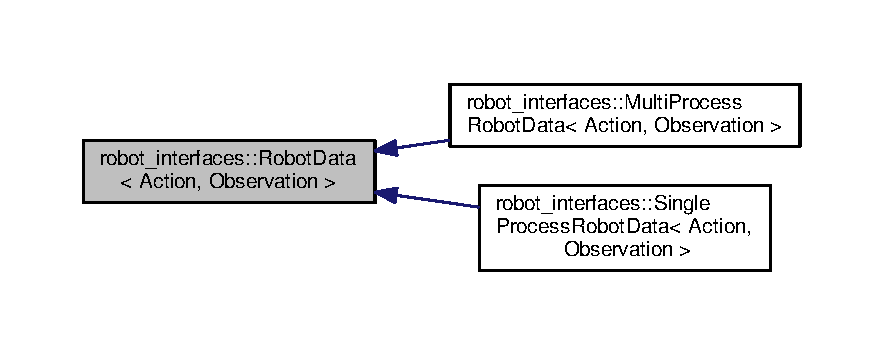
\includegraphics[width=350pt]{classrobot__interfaces_1_1RobotData__inherit__graph}
\end{center}
\end{figure}
\subsection*{Public Attributes}
\begin{DoxyCompactItemize}
\item 
std\+::shared\+\_\+ptr$<$ time\+\_\+series\+::\+Time\+Series\+Interface$<$ \hyperlink{classAction}{Action} $>$ $>$ \hyperlink{classrobot__interfaces_1_1RobotData_a03b4160b90de7eac5ffb67cb8a872cee}{desired\+\_\+action}\hypertarget{classrobot__interfaces_1_1RobotData_a03b4160b90de7eac5ffb67cb8a872cee}{}\label{classrobot__interfaces_1_1RobotData_a03b4160b90de7eac5ffb67cb8a872cee}

\begin{DoxyCompactList}\small\item\em Time series of the desired actions. \end{DoxyCompactList}\item 
std\+::shared\+\_\+ptr$<$ time\+\_\+series\+::\+Time\+Series\+Interface$<$ \hyperlink{classAction}{Action} $>$ $>$ \hyperlink{classrobot__interfaces_1_1RobotData_a05fea4d2f75f7fc34daf2bfc71fbfc4b}{applied\+\_\+action}\hypertarget{classrobot__interfaces_1_1RobotData_a05fea4d2f75f7fc34daf2bfc71fbfc4b}{}\label{classrobot__interfaces_1_1RobotData_a05fea4d2f75f7fc34daf2bfc71fbfc4b}

\begin{DoxyCompactList}\small\item\em Time series of the actually applied actions (due to safety. \end{DoxyCompactList}\item 
std\+::shared\+\_\+ptr$<$ time\+\_\+series\+::\+Time\+Series\+Interface$<$ \hyperlink{classObservation}{Observation} $>$ $>$ \hyperlink{classrobot__interfaces_1_1RobotData_ae3d13595b92f82f76b0f1df2961258bd}{observation}\hypertarget{classrobot__interfaces_1_1RobotData_ae3d13595b92f82f76b0f1df2961258bd}{}\label{classrobot__interfaces_1_1RobotData_ae3d13595b92f82f76b0f1df2961258bd}

\begin{DoxyCompactList}\small\item\em Time series of the observations retrieved from the robot. \end{DoxyCompactList}\item 
std\+::shared\+\_\+ptr$<$ time\+\_\+series\+::\+Time\+Series\+Interface$<$ \hyperlink{structrobot__interfaces_1_1Status}{Status} $>$ $>$ \hyperlink{classrobot__interfaces_1_1RobotData_a47c53daf923c30981d15008e5134f648}{status}\hypertarget{classrobot__interfaces_1_1RobotData_a47c53daf923c30981d15008e5134f648}{}\label{classrobot__interfaces_1_1RobotData_a47c53daf923c30981d15008e5134f648}

\begin{DoxyCompactList}\small\item\em Time series of status messages. \end{DoxyCompactList}\end{DoxyCompactItemize}


\subsection{Detailed Description}
\subsubsection*{template$<$typename Action, typename Observation$>$\\*
class robot\+\_\+interfaces\+::\+Robot\+Data$<$ Action, Observation $>$}

Contains all the input and output data of the robot. 

This means the
\begin{DoxyItemize}
\item {\ttfamily desired\+\_\+action} which was requested by the robot user
\item {\ttfamily applied\+\_\+action} which was actually applied and may not be and may not be identical to desired\+\_\+action for safety reasons
\item {\ttfamily observation} made by the robot
\item {\ttfamily status} which keeps track of timing issues and errors.
\end{DoxyItemize}

See this graph to understand how they relate to each other precisely in terms of time\+:

\begin{DoxyVerb}|------ t = 0 ------|------ t = 1 ------|
|----- action0 -----|----- action1 -----|
o                   o                   o
b                   b                   b
s                   s                   s
0                   1                   2
\end{DoxyVerb}



\begin{DoxyTemplParams}{Template Parameters}
{\em \hyperlink{classAction}{Action}} & Type of the actions. \\
\hline
{\em \hyperlink{classObservation}{Observation}} & Type of the observations. \\
\hline
\end{DoxyTemplParams}


The documentation for this class was generated from the following file\+:\begin{DoxyCompactItemize}
\item 
include/robot\+\_\+interfaces/\hyperlink{robot__data_8hpp}{robot\+\_\+data.\+hpp}\end{DoxyCompactItemize}

\hypertarget{classrobot__interfaces_1_1RobotDriver}{}\section{robot\+\_\+interfaces\+:\+:Robot\+Driver$<$ T\+Action, T\+Observation $>$ Class Template Reference}
\label{classrobot__interfaces_1_1RobotDriver}\index{robot\+\_\+interfaces\+::\+Robot\+Driver$<$ T\+Action, T\+Observation $>$@{robot\+\_\+interfaces\+::\+Robot\+Driver$<$ T\+Action, T\+Observation $>$}}


\hyperlink{classDriver}{Driver} for interfacing the actual robot hardware or simulation.  




{\ttfamily \#include $<$robot\+\_\+driver.\+hpp$>$}

\subsection*{Public Types}
\begin{DoxyCompactItemize}
\item 
typedef T\+Action {\bfseries Action}\hypertarget{classrobot__interfaces_1_1RobotDriver_acbba637e7857bef5c7a1e64c9846ead7}{}\label{classrobot__interfaces_1_1RobotDriver_acbba637e7857bef5c7a1e64c9846ead7}

\item 
typedef T\+Observation {\bfseries Observation}\hypertarget{classrobot__interfaces_1_1RobotDriver_abcb094711d0ae09fd8e2fc9a6aa771f2}{}\label{classrobot__interfaces_1_1RobotDriver_abcb094711d0ae09fd8e2fc9a6aa771f2}

\end{DoxyCompactItemize}
\subsection*{Public Member Functions}
\begin{DoxyCompactItemize}
\item 
virtual void \hyperlink{classrobot__interfaces_1_1RobotDriver_af3cbef570a455e1f8085d701282264ff}{initialize} ()=0
\begin{DoxyCompactList}\small\item\em Initialize the robot. \end{DoxyCompactList}\item 
virtual \hyperlink{classAction}{Action} \hyperlink{classrobot__interfaces_1_1RobotDriver_a4294e522fcd12b38d69f7d53fae5d74a}{apply\+\_\+action} (const \hyperlink{classAction}{Action} \&desired\+\_\+action)=0
\begin{DoxyCompactList}\small\item\em Apply action immediately and block until it is executed. \end{DoxyCompactList}\item 
virtual \hyperlink{classObservation}{Observation} \hyperlink{classrobot__interfaces_1_1RobotDriver_ad13d4f4fdfe78bdde4fc964f07fa45e2}{get\+\_\+latest\+\_\+observation} ()=0
\begin{DoxyCompactList}\small\item\em Return the latest observation immediately. \end{DoxyCompactList}\item 
virtual std\+::string \hyperlink{classrobot__interfaces_1_1RobotDriver_acdf4c5d6993b836a180e6b6fc12b3445}{get\+\_\+error} ()=0
\begin{DoxyCompactList}\small\item\em Get error message if there is any error. \end{DoxyCompactList}\item 
virtual void \hyperlink{classrobot__interfaces_1_1RobotDriver_a3451fb8b15d2840b559f3ee858de01f8}{shutdown} ()=0\hypertarget{classrobot__interfaces_1_1RobotDriver_a3451fb8b15d2840b559f3ee858de01f8}{}\label{classrobot__interfaces_1_1RobotDriver_a3451fb8b15d2840b559f3ee858de01f8}

\begin{DoxyCompactList}\small\item\em Shut down the robot safely. \end{DoxyCompactList}\end{DoxyCompactItemize}


\subsection{Detailed Description}
\subsubsection*{template$<$typename T\+Action, typename T\+Observation$>$\\*
class robot\+\_\+interfaces\+::\+Robot\+Driver$<$ T\+Action, T\+Observation $>$}

\hyperlink{classDriver}{Driver} for interfacing the actual robot hardware or simulation. 

Interface to the robot used by the subsequent classes. Any robot (be it real or simulation) has to derive from this class and implement the functions \hyperlink{classrobot__interfaces_1_1RobotDriver_a4294e522fcd12b38d69f7d53fae5d74a}{apply\+\_\+action()}, \hyperlink{classrobot__interfaces_1_1RobotDriver_ad13d4f4fdfe78bdde4fc964f07fa45e2}{get\+\_\+latest\+\_\+observation()} and \hyperlink{classrobot__interfaces_1_1RobotDriver_a3451fb8b15d2840b559f3ee858de01f8}{shutdown()}. This Base class provides some timing logic around those three functions. It makes sure that after the first call of \hyperlink{classrobot__interfaces_1_1RobotDriver_a4294e522fcd12b38d69f7d53fae5d74a}{apply\+\_\+action()}, it is always called again after some specified time, otherwise the \hyperlink{classrobot__interfaces_1_1RobotDriver_a3451fb8b15d2840b559f3ee858de01f8}{shutdown()} method will be called. This Base class also makes sure that the \hyperlink{classrobot__interfaces_1_1RobotDriver_a4294e522fcd12b38d69f7d53fae5d74a}{apply\+\_\+action()} function itself does not take more time than expected.


\begin{DoxyTemplParams}{Template Parameters}
{\em \hyperlink{classAction}{Action}} & \\
\hline
{\em \hyperlink{classObservation}{Observation}} & \\
\hline
\end{DoxyTemplParams}
\begin{Desc}
\item[Examples\+: ]\par
\hyperlink{demo_8cpp-example}{demo.\+cpp}, and \hyperlink{demo_multiprocess_backend_8cpp-example}{demo\+\_\+multiprocess\+\_\+backend.\+cpp}.\end{Desc}


\subsection{Member Function Documentation}
\index{robot\+\_\+interfaces\+::\+Robot\+Driver@{robot\+\_\+interfaces\+::\+Robot\+Driver}!apply\+\_\+action@{apply\+\_\+action}}
\index{apply\+\_\+action@{apply\+\_\+action}!robot\+\_\+interfaces\+::\+Robot\+Driver@{robot\+\_\+interfaces\+::\+Robot\+Driver}}
\subsubsection[{\texorpdfstring{apply\+\_\+action(const Action \&desired\+\_\+action)=0}{apply_action(const Action &desired_action)=0}}]{\setlength{\rightskip}{0pt plus 5cm}template$<$typename T\+Action, typename T\+Observation$>$ virtual {\bf Action} {\bf robot\+\_\+interfaces\+::\+Robot\+Driver}$<$ T\+Action, T\+Observation $>$\+::apply\+\_\+action (
\begin{DoxyParamCaption}
\item[{const {\bf Action} \&}]{desired\+\_\+action}
\end{DoxyParamCaption}
)\hspace{0.3cm}{\ttfamily [pure virtual]}}\hypertarget{classrobot__interfaces_1_1RobotDriver_a4294e522fcd12b38d69f7d53fae5d74a}{}\label{classrobot__interfaces_1_1RobotDriver_a4294e522fcd12b38d69f7d53fae5d74a}


Apply action immediately and block until it is executed. 

This method must apply the desired\+\_\+action immediately when it is called, and only return once the action has been executed completely. This way we can accommodate both simulators and real robots with this interface.


\begin{DoxyParams}{Parameters}
{\em desired\+\_\+action} & The action we want to apply. \\
\hline
\end{DoxyParams}
\begin{DoxyReturn}{Returns}
The action that was actually applied (since due to safety reasons it might not be possible to apply the desired action). 
\end{DoxyReturn}


Implemented in \hyperlink{classDriver_a0f8d51bef151ccc38a0cb7b226048e28}{Driver}, and \hyperlink{classDriver_a0f8d51bef151ccc38a0cb7b226048e28}{Driver}.

\index{robot\+\_\+interfaces\+::\+Robot\+Driver@{robot\+\_\+interfaces\+::\+Robot\+Driver}!get\+\_\+error@{get\+\_\+error}}
\index{get\+\_\+error@{get\+\_\+error}!robot\+\_\+interfaces\+::\+Robot\+Driver@{robot\+\_\+interfaces\+::\+Robot\+Driver}}
\subsubsection[{\texorpdfstring{get\+\_\+error()=0}{get_error()=0}}]{\setlength{\rightskip}{0pt plus 5cm}template$<$typename T\+Action, typename T\+Observation$>$ virtual std\+::string {\bf robot\+\_\+interfaces\+::\+Robot\+Driver}$<$ T\+Action, T\+Observation $>$\+::get\+\_\+error (
\begin{DoxyParamCaption}
{}
\end{DoxyParamCaption}
)\hspace{0.3cm}{\ttfamily [pure virtual]}}\hypertarget{classrobot__interfaces_1_1RobotDriver_acdf4c5d6993b836a180e6b6fc12b3445}{}\label{classrobot__interfaces_1_1RobotDriver_acdf4c5d6993b836a180e6b6fc12b3445}


Get error message if there is any error. 

\begin{DoxyReturn}{Returns}
Returns an error message or an empty string if there is no error. 
\end{DoxyReturn}


Implemented in \hyperlink{classrobot__interfaces_1_1MonitoredRobotDriver_a944425cc7e0845184f33b16405a9e61e}{robot\+\_\+interfaces\+::\+Monitored\+Robot\+Driver$<$ Driver $>$}, \hyperlink{classDriver_a6fb739b87c892c4102e838508855c0be}{Driver}, and \hyperlink{classDriver_a6fb739b87c892c4102e838508855c0be}{Driver}.

\index{robot\+\_\+interfaces\+::\+Robot\+Driver@{robot\+\_\+interfaces\+::\+Robot\+Driver}!get\+\_\+latest\+\_\+observation@{get\+\_\+latest\+\_\+observation}}
\index{get\+\_\+latest\+\_\+observation@{get\+\_\+latest\+\_\+observation}!robot\+\_\+interfaces\+::\+Robot\+Driver@{robot\+\_\+interfaces\+::\+Robot\+Driver}}
\subsubsection[{\texorpdfstring{get\+\_\+latest\+\_\+observation()=0}{get_latest_observation()=0}}]{\setlength{\rightskip}{0pt plus 5cm}template$<$typename T\+Action, typename T\+Observation$>$ virtual {\bf Observation} {\bf robot\+\_\+interfaces\+::\+Robot\+Driver}$<$ T\+Action, T\+Observation $>$\+::get\+\_\+latest\+\_\+observation (
\begin{DoxyParamCaption}
{}
\end{DoxyParamCaption}
)\hspace{0.3cm}{\ttfamily [pure virtual]}}\hypertarget{classrobot__interfaces_1_1RobotDriver_ad13d4f4fdfe78bdde4fc964f07fa45e2}{}\label{classrobot__interfaces_1_1RobotDriver_ad13d4f4fdfe78bdde4fc964f07fa45e2}


Return the latest observation immediately. 

\begin{DoxyReturn}{Returns}
\hyperlink{classObservation}{Observation} 
\end{DoxyReturn}


Implemented in \hyperlink{classrobot__interfaces_1_1MonitoredRobotDriver_a97774dddcda1038f338d18ef0b572ad8}{robot\+\_\+interfaces\+::\+Monitored\+Robot\+Driver$<$ Driver $>$}, \hyperlink{classDriver_afb09663997bffc5c694fb5aa8aca243a}{Driver}, and \hyperlink{classDriver_afb09663997bffc5c694fb5aa8aca243a}{Driver}.

\index{robot\+\_\+interfaces\+::\+Robot\+Driver@{robot\+\_\+interfaces\+::\+Robot\+Driver}!initialize@{initialize}}
\index{initialize@{initialize}!robot\+\_\+interfaces\+::\+Robot\+Driver@{robot\+\_\+interfaces\+::\+Robot\+Driver}}
\subsubsection[{\texorpdfstring{initialize()=0}{initialize()=0}}]{\setlength{\rightskip}{0pt plus 5cm}template$<$typename T\+Action, typename T\+Observation$>$ virtual void {\bf robot\+\_\+interfaces\+::\+Robot\+Driver}$<$ T\+Action, T\+Observation $>$\+::initialize (
\begin{DoxyParamCaption}
{}
\end{DoxyParamCaption}
)\hspace{0.3cm}{\ttfamily [pure virtual]}}\hypertarget{classrobot__interfaces_1_1RobotDriver_af3cbef570a455e1f8085d701282264ff}{}\label{classrobot__interfaces_1_1RobotDriver_af3cbef570a455e1f8085d701282264ff}


Initialize the robot. 

Any initialization procedures that need to be done before sending actions to the robot should be done in this method (e.\+g. homing to find the absolute position). 

Implemented in \hyperlink{classrobot__interfaces_1_1MonitoredRobotDriver_a47b68c24afaa087e4e60e6413ab7ac89}{robot\+\_\+interfaces\+::\+Monitored\+Robot\+Driver$<$ Driver $>$}, \hyperlink{classDriver_a81c0beb523fad80cd40cfcc6a6e3de2d}{Driver}, and \hyperlink{classDriver_a81c0beb523fad80cd40cfcc6a6e3de2d}{Driver}.



The documentation for this class was generated from the following file\+:\begin{DoxyCompactItemize}
\item 
include/robot\+\_\+interfaces/robot\+\_\+driver.\+hpp\end{DoxyCompactItemize}

\hypertarget{classrobot__interfaces_1_1RobotFrontend}{}\section{robot\+\_\+interfaces\+:\+:Robot\+Frontend$<$ Action, Observation $>$ Class Template Reference}
\label{classrobot__interfaces_1_1RobotFrontend}\index{robot\+\_\+interfaces\+::\+Robot\+Frontend$<$ Action, Observation $>$@{robot\+\_\+interfaces\+::\+Robot\+Frontend$<$ Action, Observation $>$}}


Communication link between \hyperlink{classrobot__interfaces_1_1RobotData}{Robot\+Data} and the user.  




{\ttfamily \#include $<$robot\+\_\+frontend.\+hpp$>$}



Inheritance diagram for robot\+\_\+interfaces\+:\+:Robot\+Frontend$<$ Action, Observation $>$\+:
\nopagebreak
\begin{figure}[H]
\begin{center}
\leavevmode
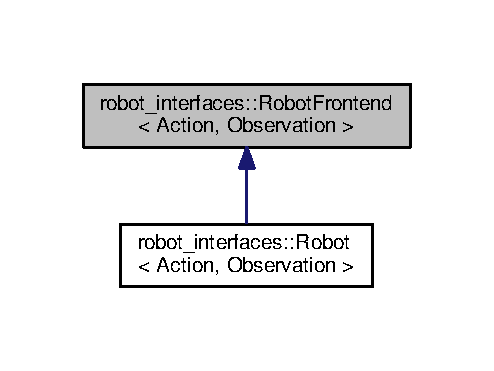
\includegraphics[width=237pt]{classrobot__interfaces_1_1RobotFrontend__inherit__graph}
\end{center}
\end{figure}
\subsection*{Public Types}
\begin{DoxyCompactItemize}
\item 
typedef time\+\_\+series\+::\+Timestamp {\bfseries Time\+Stamp}\hypertarget{classrobot__interfaces_1_1RobotFrontend_a02bebc6c3e9822f026c48f970d80a865}{}\label{classrobot__interfaces_1_1RobotFrontend_a02bebc6c3e9822f026c48f970d80a865}

\end{DoxyCompactItemize}
\subsection*{Public Member Functions}
\begin{DoxyCompactItemize}
\item 
{\bfseries Robot\+Frontend} (std\+::shared\+\_\+ptr$<$ \hyperlink{classrobot__interfaces_1_1RobotData}{Robot\+Data}$<$ \hyperlink{classAction}{Action}, \hyperlink{classObservation}{Observation} $>$$>$ robot\+\_\+data)\hypertarget{classrobot__interfaces_1_1RobotFrontend_a0bd84764fb1a3004282706963aa48c3e}{}\label{classrobot__interfaces_1_1RobotFrontend_a0bd84764fb1a3004282706963aa48c3e}

\item 
\hyperlink{classObservation}{Observation} {\bfseries get\+\_\+observation} (const Time\+Index \&t)\hypertarget{classrobot__interfaces_1_1RobotFrontend_a7628a6f8d6858bb42565ad3577b9d5f0}{}\label{classrobot__interfaces_1_1RobotFrontend_a7628a6f8d6858bb42565ad3577b9d5f0}

\item 
\hyperlink{classAction}{Action} {\bfseries get\+\_\+desired\+\_\+action} (const Time\+Index \&t)\hypertarget{classrobot__interfaces_1_1RobotFrontend_ad9cf328a6a438cf40df1944c1772fca8}{}\label{classrobot__interfaces_1_1RobotFrontend_ad9cf328a6a438cf40df1944c1772fca8}

\item 
\hyperlink{classAction}{Action} {\bfseries get\+\_\+applied\+\_\+action} (const Time\+Index \&t)\hypertarget{classrobot__interfaces_1_1RobotFrontend_a52f915a23cd37e4c108080ed5cba674a}{}\label{classrobot__interfaces_1_1RobotFrontend_a52f915a23cd37e4c108080ed5cba674a}

\item 
\hyperlink{structrobot__interfaces_1_1Status}{Status} {\bfseries get\+\_\+status} (const Time\+Index \&t)\hypertarget{classrobot__interfaces_1_1RobotFrontend_a48eff6e33cdafa175e8e311296aacfec}{}\label{classrobot__interfaces_1_1RobotFrontend_a48eff6e33cdafa175e8e311296aacfec}

\item 
Time\+Stamp {\bfseries get\+\_\+time\+\_\+stamp\+\_\+ms} (const Time\+Index \&t)\hypertarget{classrobot__interfaces_1_1RobotFrontend_abaf909237a40a0da1839d5e341ad572b}{}\label{classrobot__interfaces_1_1RobotFrontend_abaf909237a40a0da1839d5e341ad572b}

\item 
Time\+Index {\bfseries get\+\_\+current\+\_\+timeindex} ()\hypertarget{classrobot__interfaces_1_1RobotFrontend_a3d74aa3bd15ab0baef5d011f06aad7e7}{}\label{classrobot__interfaces_1_1RobotFrontend_a3d74aa3bd15ab0baef5d011f06aad7e7}

\item 
Time\+Index {\bfseries append\+\_\+desired\+\_\+action} (const \hyperlink{classAction}{Action} \&desired\+\_\+action)\hypertarget{classrobot__interfaces_1_1RobotFrontend_a26c137f65b908d6eddffff75df38361a}{}\label{classrobot__interfaces_1_1RobotFrontend_a26c137f65b908d6eddffff75df38361a}

\item 
void {\bfseries wait\+\_\+until\+\_\+timeindex} (const Time\+Index \&t)\hypertarget{classrobot__interfaces_1_1RobotFrontend_a9b5242a6781e6028a84a6eb358b1ad10}{}\label{classrobot__interfaces_1_1RobotFrontend_a9b5242a6781e6028a84a6eb358b1ad10}

\end{DoxyCompactItemize}
\subsection*{Protected Attributes}
\begin{DoxyCompactItemize}
\item 
std\+::shared\+\_\+ptr$<$ \hyperlink{classrobot__interfaces_1_1RobotData}{Robot\+Data}$<$ \hyperlink{classAction}{Action}, \hyperlink{classObservation}{Observation} $>$ $>$ {\bfseries robot\+\_\+data\+\_\+}\hypertarget{classrobot__interfaces_1_1RobotFrontend_a256d4a3359c46caca9fe92d62b4ae413}{}\label{classrobot__interfaces_1_1RobotFrontend_a256d4a3359c46caca9fe92d62b4ae413}

\end{DoxyCompactItemize}


\subsection{Detailed Description}
\subsubsection*{template$<$typename Action, typename Observation$>$\\*
class robot\+\_\+interfaces\+::\+Robot\+Frontend$<$ Action, Observation $>$}

Communication link between \hyperlink{classrobot__interfaces_1_1RobotData}{Robot\+Data} and the user. 

Takes care of communication between the \hyperlink{classrobot__interfaces_1_1RobotData}{Robot\+Data} and the user. It is just a thin wrapper around \hyperlink{classrobot__interfaces_1_1RobotData}{Robot\+Data} to facilitate interaction and also to make sure the user cannot use \hyperlink{classrobot__interfaces_1_1RobotData}{Robot\+Data} in incorrect ways.


\begin{DoxyTemplParams}{Template Parameters}
{\em \hyperlink{classAction}{Action}} & \\
\hline
{\em \hyperlink{classObservation}{Observation}} & \\
\hline
\end{DoxyTemplParams}
\begin{Desc}
\item[Examples\+: ]\par
\hyperlink{demo_8cpp-example}{demo.\+cpp}, and \hyperlink{demo_multiprocess_frontend_8cpp-example}{demo\+\_\+multiprocess\+\_\+frontend.\+cpp}.\end{Desc}


The documentation for this class was generated from the following file\+:\begin{DoxyCompactItemize}
\item 
include/robot\+\_\+interfaces/robot\+\_\+frontend.\+hpp\end{DoxyCompactItemize}

\hypertarget{classrobot__interfaces_1_1RobotLogger}{}\section{robot\+\_\+interfaces\+:\+:Robot\+Logger$<$ Action, Observation $>$ Class Template Reference}
\label{classrobot__interfaces_1_1RobotLogger}\index{robot\+\_\+interfaces\+::\+Robot\+Logger$<$ Action, Observation $>$@{robot\+\_\+interfaces\+::\+Robot\+Logger$<$ Action, Observation $>$}}


To log data from {\itshape any} robot (real, simulated, fake).  




{\ttfamily \#include $<$robot\+\_\+logger.\+hpp$>$}

\subsection*{Public Member Functions}
\begin{DoxyCompactItemize}
\item 
{\bfseries Robot\+Logger} (std\+::shared\+\_\+ptr$<$ \hyperlink{classrobot__interfaces_1_1RobotData}{robot\+\_\+interfaces\+::\+Robot\+Data}$<$ \hyperlink{classAction}{Action}, \hyperlink{classObservation}{Observation} $>$$>$ robot\+\_\+data, int block\+\_\+size)\hypertarget{classrobot__interfaces_1_1RobotLogger_a40fbf613d2fd5a54dfd71a0dde9da616}{}\label{classrobot__interfaces_1_1RobotLogger_a40fbf613d2fd5a54dfd71a0dde9da616}

\item 
std\+::vector$<$ std\+::string $>$ \hyperlink{classrobot__interfaces_1_1RobotLogger_aff9a4e9a91b3fe604bd16a94a006e151}{get\+\_\+header} ()
\begin{DoxyCompactList}\small\item\em To get the title of the log file, describing all the information that will be logged in it. \end{DoxyCompactList}\item 
void \hyperlink{classrobot__interfaces_1_1RobotLogger_a7c94db4517002755f3325c13aa430733}{append\+\_\+name\+\_\+to\+\_\+header} (std\+::string identifier, std\+::vector$<$ std\+::string $>$ field\+\_\+name, std\+::vector$<$ std\+::vector$<$ double $>$$>$ field\+\_\+data, std\+::vector$<$ std\+::string $>$ \&header)
\begin{DoxyCompactList}\small\item\em Fills in the name information of each field to be logged according to the size of the field. \end{DoxyCompactList}\item 
void \hyperlink{classrobot__interfaces_1_1RobotLogger_a8c7c9b7bff6e49b340c90b36bee9331e}{append\+\_\+header\+\_\+to\+\_\+file} ()\hypertarget{classrobot__interfaces_1_1RobotLogger_a8c7c9b7bff6e49b340c90b36bee9331e}{}\label{classrobot__interfaces_1_1RobotLogger_a8c7c9b7bff6e49b340c90b36bee9331e}

\begin{DoxyCompactList}\small\item\em Writes the header to the log file. \end{DoxyCompactList}\item 
void \hyperlink{classrobot__interfaces_1_1RobotLogger_ac568cd79a651c2c20fa9e1f136155ced}{append\+\_\+robot\+\_\+data\+\_\+to\+\_\+file} ()\hypertarget{classrobot__interfaces_1_1RobotLogger_ac568cd79a651c2c20fa9e1f136155ced}{}\label{classrobot__interfaces_1_1RobotLogger_ac568cd79a651c2c20fa9e1f136155ced}

\begin{DoxyCompactList}\small\item\em Writes the timestamped robot data at {\itshape hopefully} every time index to the log file. \end{DoxyCompactList}\item 
void \hyperlink{classrobot__interfaces_1_1RobotLogger_a70c988142c9ccbdc0c81b0bcc689031e}{append\+\_\+field\+\_\+data\+\_\+to\+\_\+file} (std\+::vector$<$ std\+::vector$<$ double $>$$>$ field\+\_\+data)
\begin{DoxyCompactList}\small\item\em Appends the data corresponding to every field at the same time index to the log file. \end{DoxyCompactList}\item 
void \hyperlink{classrobot__interfaces_1_1RobotLogger_a8dc63e66127923cfee3a2ddaf764da86}{write} ()
\begin{DoxyCompactList}\small\item\em Writes everything to the log file. \end{DoxyCompactList}\item 
void \hyperlink{classrobot__interfaces_1_1RobotLogger_a9abfad073fd735b9873b4b3f19f268e0}{start} (std\+::string filename)
\begin{DoxyCompactList}\small\item\em Call \hyperlink{classrobot__interfaces_1_1RobotLogger_a9abfad073fd735b9873b4b3f19f268e0}{start()} to create the thread for the \hyperlink{classrobot__interfaces_1_1RobotLogger}{Robot\+Logger} and start logging! \end{DoxyCompactList}\item 
void \hyperlink{classrobot__interfaces_1_1RobotLogger_a55ec7dcacd849adee53fa49a2a0c8234}{stop} ()\hypertarget{classrobot__interfaces_1_1RobotLogger_a55ec7dcacd849adee53fa49a2a0c8234}{}\label{classrobot__interfaces_1_1RobotLogger_a55ec7dcacd849adee53fa49a2a0c8234}

\begin{DoxyCompactList}\small\item\em Call \hyperlink{classrobot__interfaces_1_1RobotLogger_a55ec7dcacd849adee53fa49a2a0c8234}{stop()} when you want to stop logging. \end{DoxyCompactList}\end{DoxyCompactItemize}
\subsection*{Static Public Member Functions}
\begin{DoxyCompactItemize}
\item 
static void $\ast$ {\bfseries write} (void $\ast$instance\+\_\+pointer)\hypertarget{classrobot__interfaces_1_1RobotLogger_a909c3baf8d34945085fee9c45e9d80c4}{}\label{classrobot__interfaces_1_1RobotLogger_a909c3baf8d34945085fee9c45e9d80c4}

\end{DoxyCompactItemize}
\subsection*{Public Attributes}
\begin{DoxyCompactItemize}
\item 
std\+::shared\+\_\+ptr$<$ \hyperlink{classrobot__interfaces_1_1RobotData}{robot\+\_\+interfaces\+::\+Robot\+Data}$<$ \hyperlink{classAction}{Action}, \hyperlink{classObservation}{Observation} $>$ $>$ \hyperlink{classrobot__interfaces_1_1RobotLogger_ad1391bc38ff516f01b3c8bdd91e27efc}{logger\+\_\+data\+\_\+}
\begin{DoxyCompactList}\small\item\em This is to verify that the template types of the \hyperlink{classrobot__interfaces_1_1RobotLogger}{Robot\+Logger} are based on \hyperlink{classrobot__interfaces_1_1Loggable}{Loggable}. \end{DoxyCompactList}\item 
int {\bfseries block\+\_\+size\+\_\+}\hypertarget{classrobot__interfaces_1_1RobotLogger_a0465f86efac78a429f8980bd2a12959e}{}\label{classrobot__interfaces_1_1RobotLogger_a0465f86efac78a429f8980bd2a12959e}

\item 
long int {\bfseries index\+\_\+}\hypertarget{classrobot__interfaces_1_1RobotLogger_ac47398855bcb94ca8a3e83334ee1d382}{}\label{classrobot__interfaces_1_1RobotLogger_ac47398855bcb94ca8a3e83334ee1d382}

\item 
bool {\bfseries stop\+\_\+was\+\_\+called\+\_\+}\hypertarget{classrobot__interfaces_1_1RobotLogger_a133c310dcabe26cb8918dad08ed96a90}{}\label{classrobot__interfaces_1_1RobotLogger_a133c310dcabe26cb8918dad08ed96a90}

\item 
std\+::ofstream {\bfseries output\+\_\+file\+\_\+}\hypertarget{classrobot__interfaces_1_1RobotLogger_aa03a18fb24545744533c39e193c5920a}{}\label{classrobot__interfaces_1_1RobotLogger_aa03a18fb24545744533c39e193c5920a}

\item 
std\+::string {\bfseries output\+\_\+file\+\_\+name\+\_\+}\hypertarget{classrobot__interfaces_1_1RobotLogger_a180a1ad565fd1a2342c6a40465fea731}{}\label{classrobot__interfaces_1_1RobotLogger_a180a1ad565fd1a2342c6a40465fea731}

\end{DoxyCompactItemize}
\subsection*{Private Attributes}
\begin{DoxyCompactItemize}
\item 
std\+::shared\+\_\+ptr$<$ real\+\_\+time\+\_\+tools\+::\+Real\+Time\+Thread $>$ {\bfseries thread\+\_\+}\hypertarget{classrobot__interfaces_1_1RobotLogger_a6a9d7845a73b1d62d0f0ddf85240c336}{}\label{classrobot__interfaces_1_1RobotLogger_a6a9d7845a73b1d62d0f0ddf85240c336}

\end{DoxyCompactItemize}


\subsection{Detailed Description}
\subsubsection*{template$<$typename Action, typename Observation$>$\\*
class robot\+\_\+interfaces\+::\+Robot\+Logger$<$ Action, Observation $>$}

To log data from {\itshape any} robot (real, simulated, fake). 

The \hyperlink{classrobot__interfaces_1_1RobotLogger}{Robot\+Logger} logs the timestamp, the time index, and the values of every \hyperlink{classObservation}{Observation}, \hyperlink{classAction}{Action}, and \hyperlink{structrobot__interfaces_1_1Status}{Status} variable. \hyperlink{classObservation}{Observation}, \hyperlink{classAction}{Action}, and \hyperlink{structrobot__interfaces_1_1Status}{Status} {\itshape must} derive from \hyperlink{classrobot__interfaces_1_1Loggable}{Loggable}. Any further data structure can be logged similarly, which derives from \hyperlink{classrobot__interfaces_1_1Loggable}{Loggable}.


\begin{DoxyTemplParams}{Template Parameters}
{\em \hyperlink{classAction}{Action}} & \\
\hline
{\em \hyperlink{classObservation}{Observation}} & \\
\hline
\end{DoxyTemplParams}


\subsection{Member Function Documentation}
\index{robot\+\_\+interfaces\+::\+Robot\+Logger@{robot\+\_\+interfaces\+::\+Robot\+Logger}!append\+\_\+field\+\_\+data\+\_\+to\+\_\+file@{append\+\_\+field\+\_\+data\+\_\+to\+\_\+file}}
\index{append\+\_\+field\+\_\+data\+\_\+to\+\_\+file@{append\+\_\+field\+\_\+data\+\_\+to\+\_\+file}!robot\+\_\+interfaces\+::\+Robot\+Logger@{robot\+\_\+interfaces\+::\+Robot\+Logger}}
\subsubsection[{\texorpdfstring{append\+\_\+field\+\_\+data\+\_\+to\+\_\+file(std\+::vector$<$ std\+::vector$<$ double $>$$>$ field\+\_\+data)}{append_field_data_to_file(std::vector< std::vector< double >> field_data)}}]{\setlength{\rightskip}{0pt plus 5cm}template$<$typename Action , typename Observation $>$ void {\bf robot\+\_\+interfaces\+::\+Robot\+Logger}$<$ {\bf Action}, {\bf Observation} $>$\+::append\+\_\+field\+\_\+data\+\_\+to\+\_\+file (
\begin{DoxyParamCaption}
\item[{std\+::vector$<$ std\+::vector$<$ double $>$$>$}]{field\+\_\+data}
\end{DoxyParamCaption}
)\hspace{0.3cm}{\ttfamily [inline]}}\hypertarget{classrobot__interfaces_1_1RobotLogger_a70c988142c9ccbdc0c81b0bcc689031e}{}\label{classrobot__interfaces_1_1RobotLogger_a70c988142c9ccbdc0c81b0bcc689031e}


Appends the data corresponding to every field at the same time index to the log file. 


\begin{DoxyParams}{Parameters}
{\em field\+\_\+data} & The field data \\
\hline
\end{DoxyParams}
\index{robot\+\_\+interfaces\+::\+Robot\+Logger@{robot\+\_\+interfaces\+::\+Robot\+Logger}!append\+\_\+name\+\_\+to\+\_\+header@{append\+\_\+name\+\_\+to\+\_\+header}}
\index{append\+\_\+name\+\_\+to\+\_\+header@{append\+\_\+name\+\_\+to\+\_\+header}!robot\+\_\+interfaces\+::\+Robot\+Logger@{robot\+\_\+interfaces\+::\+Robot\+Logger}}
\subsubsection[{\texorpdfstring{append\+\_\+name\+\_\+to\+\_\+header(std\+::string identifier, std\+::vector$<$ std\+::string $>$ field\+\_\+name, std\+::vector$<$ std\+::vector$<$ double $>$$>$ field\+\_\+data, std\+::vector$<$ std\+::string $>$ \&header)}{append_name_to_header(std::string identifier, std::vector< std::string > field_name, std::vector< std::vector< double >> field_data, std::vector< std::string > &header)}}]{\setlength{\rightskip}{0pt plus 5cm}template$<$typename Action , typename Observation $>$ void {\bf robot\+\_\+interfaces\+::\+Robot\+Logger}$<$ {\bf Action}, {\bf Observation} $>$\+::append\+\_\+name\+\_\+to\+\_\+header (
\begin{DoxyParamCaption}
\item[{std\+::string}]{identifier, }
\item[{std\+::vector$<$ std\+::string $>$}]{field\+\_\+name, }
\item[{std\+::vector$<$ std\+::vector$<$ double $>$$>$}]{field\+\_\+data, }
\item[{std\+::vector$<$ std\+::string $>$ \&}]{header}
\end{DoxyParamCaption}
)\hspace{0.3cm}{\ttfamily [inline]}}\hypertarget{classrobot__interfaces_1_1RobotLogger_a7c94db4517002755f3325c13aa430733}{}\label{classrobot__interfaces_1_1RobotLogger_a7c94db4517002755f3325c13aa430733}


Fills in the name information of each field to be logged according to the size of the field. 


\begin{DoxyParams}{Parameters}
{\em identifier} & The structure the field corresponds to \\
\hline
{\em field\+\_\+name} & The name of the field \\
\hline
{\em field\+\_\+data} & The field data \\
\hline
{\em \&header} & Reference to the header of the log file \\
\hline
\end{DoxyParams}
\index{robot\+\_\+interfaces\+::\+Robot\+Logger@{robot\+\_\+interfaces\+::\+Robot\+Logger}!get\+\_\+header@{get\+\_\+header}}
\index{get\+\_\+header@{get\+\_\+header}!robot\+\_\+interfaces\+::\+Robot\+Logger@{robot\+\_\+interfaces\+::\+Robot\+Logger}}
\subsubsection[{\texorpdfstring{get\+\_\+header()}{get_header()}}]{\setlength{\rightskip}{0pt plus 5cm}template$<$typename Action , typename Observation $>$ std\+::vector$<$std\+::string$>$ {\bf robot\+\_\+interfaces\+::\+Robot\+Logger}$<$ {\bf Action}, {\bf Observation} $>$\+::get\+\_\+header (
\begin{DoxyParamCaption}
{}
\end{DoxyParamCaption}
)\hspace{0.3cm}{\ttfamily [inline]}}\hypertarget{classrobot__interfaces_1_1RobotLogger_aff9a4e9a91b3fe604bd16a94a006e151}{}\label{classrobot__interfaces_1_1RobotLogger_aff9a4e9a91b3fe604bd16a94a006e151}


To get the title of the log file, describing all the information that will be logged in it. 

\begin{DoxyReturn}{Returns}
header The title of the log file. 
\end{DoxyReturn}
\index{robot\+\_\+interfaces\+::\+Robot\+Logger@{robot\+\_\+interfaces\+::\+Robot\+Logger}!start@{start}}
\index{start@{start}!robot\+\_\+interfaces\+::\+Robot\+Logger@{robot\+\_\+interfaces\+::\+Robot\+Logger}}
\subsubsection[{\texorpdfstring{start(std\+::string filename)}{start(std::string filename)}}]{\setlength{\rightskip}{0pt plus 5cm}template$<$typename Action , typename Observation $>$ void {\bf robot\+\_\+interfaces\+::\+Robot\+Logger}$<$ {\bf Action}, {\bf Observation} $>$\+::start (
\begin{DoxyParamCaption}
\item[{std\+::string}]{filename}
\end{DoxyParamCaption}
)\hspace{0.3cm}{\ttfamily [inline]}}\hypertarget{classrobot__interfaces_1_1RobotLogger_a9abfad073fd735b9873b4b3f19f268e0}{}\label{classrobot__interfaces_1_1RobotLogger_a9abfad073fd735b9873b4b3f19f268e0}


Call \hyperlink{classrobot__interfaces_1_1RobotLogger_a9abfad073fd735b9873b4b3f19f268e0}{start()} to create the thread for the \hyperlink{classrobot__interfaces_1_1RobotLogger}{Robot\+Logger} and start logging! 

\begin{DoxyNote}{Note}
Every time you start the logger with the same file name, it will obviously append newer data to the same file. This shouldn\textquotesingle{}t be a problem. But for different log files, specify different file names while starting the logger.
\end{DoxyNote}

\begin{DoxyParams}{Parameters}
{\em filename} & The name of the log file. \\
\hline
\end{DoxyParams}
\index{robot\+\_\+interfaces\+::\+Robot\+Logger@{robot\+\_\+interfaces\+::\+Robot\+Logger}!write@{write}}
\index{write@{write}!robot\+\_\+interfaces\+::\+Robot\+Logger@{robot\+\_\+interfaces\+::\+Robot\+Logger}}
\subsubsection[{\texorpdfstring{write()}{write()}}]{\setlength{\rightskip}{0pt plus 5cm}template$<$typename Action , typename Observation $>$ void {\bf robot\+\_\+interfaces\+::\+Robot\+Logger}$<$ {\bf Action}, {\bf Observation} $>$\+::write (
\begin{DoxyParamCaption}
{}
\end{DoxyParamCaption}
)\hspace{0.3cm}{\ttfamily [inline]}}\hypertarget{classrobot__interfaces_1_1RobotLogger_a8dc63e66127923cfee3a2ddaf764da86}{}\label{classrobot__interfaces_1_1RobotLogger_a8dc63e66127923cfee3a2ddaf764da86}


Writes everything to the log file. 

It dumps all the data corresponding to block\+\_\+size\+\_\+ number of time indices at one go. 

\subsection{Member Data Documentation}
\index{robot\+\_\+interfaces\+::\+Robot\+Logger@{robot\+\_\+interfaces\+::\+Robot\+Logger}!logger\+\_\+data\+\_\+@{logger\+\_\+data\+\_\+}}
\index{logger\+\_\+data\+\_\+@{logger\+\_\+data\+\_\+}!robot\+\_\+interfaces\+::\+Robot\+Logger@{robot\+\_\+interfaces\+::\+Robot\+Logger}}
\subsubsection[{\texorpdfstring{logger\+\_\+data\+\_\+}{logger_data_}}]{\setlength{\rightskip}{0pt plus 5cm}template$<$typename Action , typename Observation $>$ std\+::shared\+\_\+ptr$<${\bf robot\+\_\+interfaces\+::\+Robot\+Data}$<${\bf Action}, {\bf Observation}$>$ $>$ {\bf robot\+\_\+interfaces\+::\+Robot\+Logger}$<$ {\bf Action}, {\bf Observation} $>$\+::logger\+\_\+data\+\_\+}\hypertarget{classrobot__interfaces_1_1RobotLogger_ad1391bc38ff516f01b3c8bdd91e27efc}{}\label{classrobot__interfaces_1_1RobotLogger_ad1391bc38ff516f01b3c8bdd91e27efc}


This is to verify that the template types of the \hyperlink{classrobot__interfaces_1_1RobotLogger}{Robot\+Logger} are based on \hyperlink{classrobot__interfaces_1_1Loggable}{Loggable}. 

Currently, the level of generalisability of the logger is that we {\itshape know} the following four timeseries structures exist for {\itshape any} robot whose data is to be logged-\/ applied\+\_\+action and desired\+\_\+action (of type \hyperlink{classAction}{Action}), observation (of type \hyperlink{classObservation}{Observation}), and status (of type \hyperlink{structrobot__interfaces_1_1Status}{Status}). 

The documentation for this class was generated from the following file\+:\begin{DoxyCompactItemize}
\item 
include/robot\+\_\+interfaces/robot\+\_\+logger.\+hpp\end{DoxyCompactItemize}

\hypertarget{classrobot__interfaces_1_1SensorBackend}{}\section{robot\+\_\+interfaces\+:\+:Sensor\+Backend$<$ Observation\+Type $>$ Class Template Reference}
\label{classrobot__interfaces_1_1SensorBackend}\index{robot\+\_\+interfaces\+::\+Sensor\+Backend$<$ Observation\+Type $>$@{robot\+\_\+interfaces\+::\+Sensor\+Backend$<$ Observation\+Type $>$}}


Communication link between \hyperlink{classrobot__interfaces_1_1SensorData}{Sensor\+Data} and \hyperlink{classrobot__interfaces_1_1SensorDriver}{Sensor\+Driver}.  




{\ttfamily \#include $<$sensor\+\_\+backend.\+hpp$>$}

\subsection*{Public Member Functions}
\begin{DoxyCompactItemize}
\item 
\hyperlink{classrobot__interfaces_1_1SensorBackend_af24fda0e1d54274cf8122195f82acea9}{Sensor\+Backend} (std\+::shared\+\_\+ptr$<$ \hyperlink{classrobot__interfaces_1_1SensorDriver}{Sensor\+Driver}$<$ Observation\+Type $>$$>$ sensor\+\_\+driver, std\+::shared\+\_\+ptr$<$ \hyperlink{classrobot__interfaces_1_1SensorData}{Sensor\+Data}$<$ Observation\+Type $>$$>$ sensor\+\_\+data)
\end{DoxyCompactItemize}
\subsection*{Private Member Functions}
\begin{DoxyCompactItemize}
\item 
void \hyperlink{classrobot__interfaces_1_1SensorBackend_aee2c015c331cf8acd80b57523f10beaa}{loop} ()\hypertarget{classrobot__interfaces_1_1SensorBackend_aee2c015c331cf8acd80b57523f10beaa}{}\label{classrobot__interfaces_1_1SensorBackend_aee2c015c331cf8acd80b57523f10beaa}

\begin{DoxyCompactList}\small\item\em Main loop. \end{DoxyCompactList}\end{DoxyCompactItemize}
\subsection*{Private Attributes}
\begin{DoxyCompactItemize}
\item 
std\+::shared\+\_\+ptr$<$ \hyperlink{classrobot__interfaces_1_1SensorDriver}{Sensor\+Driver}$<$ Observation\+Type $>$ $>$ {\bfseries sensor\+\_\+driver\+\_\+}\hypertarget{classrobot__interfaces_1_1SensorBackend_a72fda090e697edcda5f92d7542788171}{}\label{classrobot__interfaces_1_1SensorBackend_a72fda090e697edcda5f92d7542788171}

\item 
std\+::shared\+\_\+ptr$<$ \hyperlink{classrobot__interfaces_1_1SensorData}{Sensor\+Data}$<$ Observation\+Type $>$ $>$ {\bfseries sensor\+\_\+data\+\_\+}\hypertarget{classrobot__interfaces_1_1SensorBackend_a93c993a56270f282235df08337e0bc26}{}\label{classrobot__interfaces_1_1SensorBackend_a93c993a56270f282235df08337e0bc26}

\item 
bool {\bfseries destructor\+\_\+was\+\_\+called\+\_\+}\hypertarget{classrobot__interfaces_1_1SensorBackend_a479d96dc0a9fce6c72c7957e005530f7}{}\label{classrobot__interfaces_1_1SensorBackend_a479d96dc0a9fce6c72c7957e005530f7}

\item 
std\+::thread {\bfseries thread\+\_\+}\hypertarget{classrobot__interfaces_1_1SensorBackend_ac9ca3c3602264de39a6bca792b51dcd4}{}\label{classrobot__interfaces_1_1SensorBackend_ac9ca3c3602264de39a6bca792b51dcd4}

\end{DoxyCompactItemize}


\subsection{Detailed Description}
\subsubsection*{template$<$typename Observation\+Type$>$\\*
class robot\+\_\+interfaces\+::\+Sensor\+Backend$<$ Observation\+Type $>$}

Communication link between \hyperlink{classrobot__interfaces_1_1SensorData}{Sensor\+Data} and \hyperlink{classrobot__interfaces_1_1SensorDriver}{Sensor\+Driver}. 

At each instant, it checks if the sensor can be accessed, and then gets the observation from it (the observation type depends on the sensor) and appends it to the sensor data.


\begin{DoxyTemplParams}{Template Parameters}
{\em Observation\+Type} & \\
\hline
\end{DoxyTemplParams}


\subsection{Constructor \& Destructor Documentation}
\index{robot\+\_\+interfaces\+::\+Sensor\+Backend@{robot\+\_\+interfaces\+::\+Sensor\+Backend}!Sensor\+Backend@{Sensor\+Backend}}
\index{Sensor\+Backend@{Sensor\+Backend}!robot\+\_\+interfaces\+::\+Sensor\+Backend@{robot\+\_\+interfaces\+::\+Sensor\+Backend}}
\subsubsection[{\texorpdfstring{Sensor\+Backend(std\+::shared\+\_\+ptr$<$ Sensor\+Driver$<$ Observation\+Type $>$$>$ sensor\+\_\+driver, std\+::shared\+\_\+ptr$<$ Sensor\+Data$<$ Observation\+Type $>$$>$ sensor\+\_\+data)}{SensorBackend(std::shared_ptr< SensorDriver< ObservationType >> sensor_driver, std::shared_ptr< SensorData< ObservationType >> sensor_data)}}]{\setlength{\rightskip}{0pt plus 5cm}template$<$typename Observation\+Type $>$ {\bf robot\+\_\+interfaces\+::\+Sensor\+Backend}$<$ Observation\+Type $>$\+::{\bf Sensor\+Backend} (
\begin{DoxyParamCaption}
\item[{std\+::shared\+\_\+ptr$<$ {\bf Sensor\+Driver}$<$ Observation\+Type $>$$>$}]{sensor\+\_\+driver, }
\item[{std\+::shared\+\_\+ptr$<$ {\bf Sensor\+Data}$<$ Observation\+Type $>$$>$}]{sensor\+\_\+data}
\end{DoxyParamCaption}
)\hspace{0.3cm}{\ttfamily [inline]}}\hypertarget{classrobot__interfaces_1_1SensorBackend_af24fda0e1d54274cf8122195f82acea9}{}\label{classrobot__interfaces_1_1SensorBackend_af24fda0e1d54274cf8122195f82acea9}

\begin{DoxyParams}{Parameters}
{\em sensor\+\_\+driver} & \hyperlink{classDriver}{Driver} instance for the sensor. \\
\hline
{\em sensor\+\_\+data} & Data is sent to/retrieved from here. \\
\hline
\end{DoxyParams}


The documentation for this class was generated from the following file\+:\begin{DoxyCompactItemize}
\item 
include/robot\+\_\+interfaces/sensors/\hyperlink{sensor__backend_8hpp}{sensor\+\_\+backend.\+hpp}\end{DoxyCompactItemize}

\hypertarget{classrobot__interfaces_1_1SensorData}{}\section{robot\+\_\+interfaces\+:\+:Sensor\+Data$<$ Observation\+Type $>$ Class Template Reference}
\label{classrobot__interfaces_1_1SensorData}\index{robot\+\_\+interfaces\+::\+Sensor\+Data$<$ Observation\+Type $>$@{robot\+\_\+interfaces\+::\+Sensor\+Data$<$ Observation\+Type $>$}}


Contains all the data coming from the sensors.  




{\ttfamily \#include $<$sensor\+\_\+data.\+hpp$>$}

\subsection*{Public Types}
\begin{DoxyCompactItemize}
\item 
{\footnotesize template$<$typename Type $>$ }\\using {\bfseries Ptr} = std\+::shared\+\_\+ptr$<$ Type $>$\hypertarget{classrobot__interfaces_1_1SensorData_a3bcc04997ea43afa13c7fdafe231818c}{}\label{classrobot__interfaces_1_1SensorData_a3bcc04997ea43afa13c7fdafe231818c}

\item 
{\footnotesize template$<$typename Type $>$ }\\using {\bfseries Timeseries} = time\+\_\+series\+::\+Time\+Series$<$ Type $>$\hypertarget{classrobot__interfaces_1_1SensorData_a3083518bc6f7fb8baf625a1551044088}{}\label{classrobot__interfaces_1_1SensorData_a3083518bc6f7fb8baf625a1551044088}

\end{DoxyCompactItemize}
\subsection*{Public Member Functions}
\begin{DoxyCompactItemize}
\item 
{\bfseries Sensor\+Data} (size\+\_\+t history\+\_\+length=15000, bool use\+\_\+shared\+\_\+memory=false, \+\_\+\+\_\+attribute\+\_\+\+\_\+((unused)) std\+::string shared\+\_\+memory\+\_\+address=\char`\"{}\char`\"{})\hypertarget{classrobot__interfaces_1_1SensorData_a386f5c340d91c2ad8f484a642c91ee86}{}\label{classrobot__interfaces_1_1SensorData_a386f5c340d91c2ad8f484a642c91ee86}

\end{DoxyCompactItemize}
\subsection*{Public Attributes}
\begin{DoxyCompactItemize}
\item 
Ptr$<$ Timeseries$<$ Observation\+Type $>$ $>$ {\bfseries observation}\hypertarget{classrobot__interfaces_1_1SensorData_a9e8e89e8583883ab1c84cbd72bea7440}{}\label{classrobot__interfaces_1_1SensorData_a9e8e89e8583883ab1c84cbd72bea7440}

\end{DoxyCompactItemize}


\subsection{Detailed Description}
\subsubsection*{template$<$typename Observation\+Type$>$\\*
class robot\+\_\+interfaces\+::\+Sensor\+Data$<$ Observation\+Type $>$}

Contains all the data coming from the sensors. 


\begin{DoxyTemplParams}{Template Parameters}
{\em Observation\+Type} & \\
\hline
\end{DoxyTemplParams}


The documentation for this class was generated from the following file\+:\begin{DoxyCompactItemize}
\item 
include/robot\+\_\+interfaces/sensors/\hyperlink{sensor__data_8hpp}{sensor\+\_\+data.\+hpp}\end{DoxyCompactItemize}

\hypertarget{classrobot__interfaces_1_1SensorDriver}{}\section{robot\+\_\+interfaces\+:\+:Sensor\+Driver$<$ Observation\+Type $>$ Class Template Reference}
\label{classrobot__interfaces_1_1SensorDriver}\index{robot\+\_\+interfaces\+::\+Sensor\+Driver$<$ Observation\+Type $>$@{robot\+\_\+interfaces\+::\+Sensor\+Driver$<$ Observation\+Type $>$}}


Base driver class from which all specific sensor drivers should derive.  




{\ttfamily \#include $<$sensor\+\_\+driver.\+hpp$>$}

\subsection*{Public Member Functions}
\begin{DoxyCompactItemize}
\item 
virtual Observation\+Type \hyperlink{classrobot__interfaces_1_1SensorDriver_a59a9918c43ba789dffb6e59f9790c6c2}{get\+\_\+observation} ()=0
\begin{DoxyCompactList}\small\item\em return the observation \end{DoxyCompactList}\end{DoxyCompactItemize}


\subsection{Detailed Description}
\subsubsection*{template$<$typename Observation\+Type$>$\\*
class robot\+\_\+interfaces\+::\+Sensor\+Driver$<$ Observation\+Type $>$}

Base driver class from which all specific sensor drivers should derive. 


\begin{DoxyTemplParams}{Template Parameters}
{\em Observation\+Type} & \\
\hline
\end{DoxyTemplParams}


\subsection{Member Function Documentation}
\index{robot\+\_\+interfaces\+::\+Sensor\+Driver@{robot\+\_\+interfaces\+::\+Sensor\+Driver}!get\+\_\+observation@{get\+\_\+observation}}
\index{get\+\_\+observation@{get\+\_\+observation}!robot\+\_\+interfaces\+::\+Sensor\+Driver@{robot\+\_\+interfaces\+::\+Sensor\+Driver}}
\subsubsection[{\texorpdfstring{get\+\_\+observation()=0}{get_observation()=0}}]{\setlength{\rightskip}{0pt plus 5cm}template$<$typename Observation\+Type $>$ virtual Observation\+Type {\bf robot\+\_\+interfaces\+::\+Sensor\+Driver}$<$ Observation\+Type $>$\+::get\+\_\+observation (
\begin{DoxyParamCaption}
{}
\end{DoxyParamCaption}
)\hspace{0.3cm}{\ttfamily [pure virtual]}}\hypertarget{classrobot__interfaces_1_1SensorDriver_a59a9918c43ba789dffb6e59f9790c6c2}{}\label{classrobot__interfaces_1_1SensorDriver_a59a9918c43ba789dffb6e59f9790c6c2}


return the observation 

\begin{DoxyReturn}{Returns}
depends on the observation structure of the sensor being interacted with 
\end{DoxyReturn}


The documentation for this class was generated from the following file\+:\begin{DoxyCompactItemize}
\item 
include/robot\+\_\+interfaces/sensors/\hyperlink{sensor__driver_8hpp}{sensor\+\_\+driver.\+hpp}\end{DoxyCompactItemize}

\hypertarget{classrobot__interfaces_1_1SensorFrontend}{}\section{robot\+\_\+interfaces\+:\+:Sensor\+Frontend$<$ Observation\+Type $>$ Class Template Reference}
\label{classrobot__interfaces_1_1SensorFrontend}\index{robot\+\_\+interfaces\+::\+Sensor\+Frontend$<$ Observation\+Type $>$@{robot\+\_\+interfaces\+::\+Sensor\+Frontend$<$ Observation\+Type $>$}}


Communication link between \hyperlink{classrobot__interfaces_1_1SensorData}{Sensor\+Data} and the user.  




{\ttfamily \#include $<$sensor\+\_\+frontend.\+hpp$>$}

\subsection*{Public Types}
\begin{DoxyCompactItemize}
\item 
{\footnotesize template$<$typename Type $>$ }\\using {\bfseries Timeseries} = time\+\_\+series\+::\+Time\+Series$<$ Type $>$\hypertarget{classrobot__interfaces_1_1SensorFrontend_a92f23f72c62ac7d32ca10742ddc5019f}{}\label{classrobot__interfaces_1_1SensorFrontend_a92f23f72c62ac7d32ca10742ddc5019f}

\item 
typedef time\+\_\+series\+::\+Timestamp {\bfseries Time\+Stamp}\hypertarget{classrobot__interfaces_1_1SensorFrontend_a28f5b6f4a74b1fd3fcd45fde6df6f0f6}{}\label{classrobot__interfaces_1_1SensorFrontend_a28f5b6f4a74b1fd3fcd45fde6df6f0f6}

\item 
typedef time\+\_\+series\+::\+Index {\bfseries Time\+Index}\hypertarget{classrobot__interfaces_1_1SensorFrontend_a199456a7768dfeec4a5c4d2a59461b8d}{}\label{classrobot__interfaces_1_1SensorFrontend_a199456a7768dfeec4a5c4d2a59461b8d}

\end{DoxyCompactItemize}
\subsection*{Public Member Functions}
\begin{DoxyCompactItemize}
\item 
{\bfseries Sensor\+Frontend} (std\+::shared\+\_\+ptr$<$ \hyperlink{classrobot__interfaces_1_1SensorData}{Sensor\+Data}$<$ Observation\+Type $>$$>$ sensor\+\_\+data)\hypertarget{classrobot__interfaces_1_1SensorFrontend_a87a137bd1903267ab407718ecc8375de}{}\label{classrobot__interfaces_1_1SensorFrontend_a87a137bd1903267ab407718ecc8375de}

\item 
Observation\+Type {\bfseries get\+\_\+observation} (const Time\+Index \&t)\hypertarget{classrobot__interfaces_1_1SensorFrontend_a5cd0e27368bdd233f1d4091448244330}{}\label{classrobot__interfaces_1_1SensorFrontend_a5cd0e27368bdd233f1d4091448244330}

\item 
Observation\+Type {\bfseries get\+\_\+latest\+\_\+observation} ()\hypertarget{classrobot__interfaces_1_1SensorFrontend_adb8f1281c2cfc36c371e9538bd030bf4}{}\label{classrobot__interfaces_1_1SensorFrontend_adb8f1281c2cfc36c371e9538bd030bf4}

\item 
Time\+Stamp {\bfseries get\+\_\+timestamp\+\_\+ms} (const Time\+Index \&t)\hypertarget{classrobot__interfaces_1_1SensorFrontend_a5b5e173a9322758e29002e5a6f536edb}{}\label{classrobot__interfaces_1_1SensorFrontend_a5b5e173a9322758e29002e5a6f536edb}

\item 
Time\+Index {\bfseries get\+\_\+current\+\_\+timeindex} ()\hypertarget{classrobot__interfaces_1_1SensorFrontend_aa1eeffc227854dc5fdede71dd04bcaa6}{}\label{classrobot__interfaces_1_1SensorFrontend_aa1eeffc227854dc5fdede71dd04bcaa6}

\end{DoxyCompactItemize}
\subsection*{Private Attributes}
\begin{DoxyCompactItemize}
\item 
std\+::shared\+\_\+ptr$<$ \hyperlink{classrobot__interfaces_1_1SensorData}{Sensor\+Data}$<$ Observation\+Type $>$ $>$ {\bfseries sensor\+\_\+data\+\_\+}\hypertarget{classrobot__interfaces_1_1SensorFrontend_a19b1505aed15c8e8e62c47e5de37d27f}{}\label{classrobot__interfaces_1_1SensorFrontend_a19b1505aed15c8e8e62c47e5de37d27f}

\end{DoxyCompactItemize}


\subsection{Detailed Description}
\subsubsection*{template$<$typename Observation\+Type$>$\\*
class robot\+\_\+interfaces\+::\+Sensor\+Frontend$<$ Observation\+Type $>$}

Communication link between \hyperlink{classrobot__interfaces_1_1SensorData}{Sensor\+Data} and the user. 

Exposes the sensor data to the user to enable the user to get observations, timestamps, and timeindices from the timeseries.


\begin{DoxyTemplParams}{Template Parameters}
{\em Observation\+Type} & \\
\hline
\end{DoxyTemplParams}


The documentation for this class was generated from the following file\+:\begin{DoxyCompactItemize}
\item 
include/robot\+\_\+interfaces/sensors/\hyperlink{sensor__frontend_8hpp}{sensor\+\_\+frontend.\+hpp}\end{DoxyCompactItemize}

\hypertarget{classrobot__interfaces_1_1SingleProcessRobotData}{}\section{robot\+\_\+interfaces\+:\+:Single\+Process\+Robot\+Data$<$ Action, Observation $>$ Class Template Reference}
\label{classrobot__interfaces_1_1SingleProcessRobotData}\index{robot\+\_\+interfaces\+::\+Single\+Process\+Robot\+Data$<$ Action, Observation $>$@{robot\+\_\+interfaces\+::\+Single\+Process\+Robot\+Data$<$ Action, Observation $>$}}


\hyperlink{classrobot__interfaces_1_1RobotData}{Robot\+Data} instance using single process time series.  




{\ttfamily \#include $<$robot\+\_\+data.\+hpp$>$}



Inheritance diagram for robot\+\_\+interfaces\+:\+:Single\+Process\+Robot\+Data$<$ Action, Observation $>$\+:
\nopagebreak
\begin{figure}[H]
\begin{center}
\leavevmode
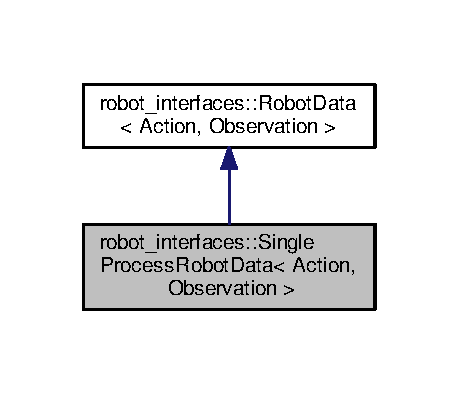
\includegraphics[width=220pt]{classrobot__interfaces_1_1SingleProcessRobotData__inherit__graph}
\end{center}
\end{figure}


Collaboration diagram for robot\+\_\+interfaces\+:\+:Single\+Process\+Robot\+Data$<$ Action, Observation $>$\+:
\nopagebreak
\begin{figure}[H]
\begin{center}
\leavevmode
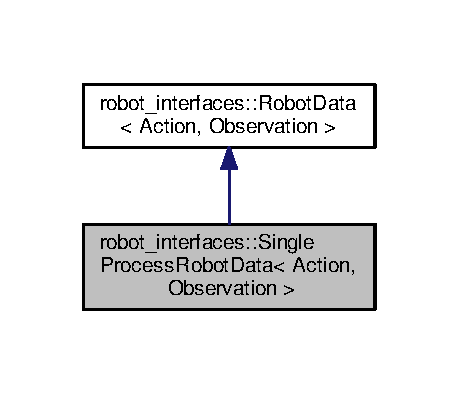
\includegraphics[width=220pt]{classrobot__interfaces_1_1SingleProcessRobotData__coll__graph}
\end{center}
\end{figure}
\subsection*{Public Member Functions}
\begin{DoxyCompactItemize}
\item 
\hyperlink{classrobot__interfaces_1_1SingleProcessRobotData_adcb9896c90464e27fb1cd2f303ca7cef}{Single\+Process\+Robot\+Data} (size\+\_\+t history\+\_\+length=1000)
\begin{DoxyCompactList}\small\item\em Construct the time series for the robot data. \end{DoxyCompactList}\end{DoxyCompactItemize}
\subsection*{Additional Inherited Members}


\subsection{Detailed Description}
\subsubsection*{template$<$typename Action, typename Observation$>$\\*
class robot\+\_\+interfaces\+::\+Single\+Process\+Robot\+Data$<$ Action, Observation $>$}

\hyperlink{classrobot__interfaces_1_1RobotData}{Robot\+Data} instance using single process time series. 

Use this class if all modules accessing the data are running in the same process. If modules run in separate processes, use \hyperlink{classrobot__interfaces_1_1MultiProcessRobotData}{Multi\+Process\+Robot\+Data} instead.

Contains all the input and output data of the robot. This means the
\begin{DoxyItemize}
\item {\ttfamily desired\+\_\+action} which was requested by the robot user
\item {\ttfamily applied\+\_\+action} which was actually applied and may not be and may not be identical to desired\+\_\+action for safety reasons
\item {\ttfamily observation} made by the robot
\item {\ttfamily status} which keeps track of timing issues and errors.
\end{DoxyItemize}

See this graph to understand how they relate to each other precisely in terms of time\+:

\begin{DoxyVerb}|------ t = 0 ------|------ t = 1 ------|
|----- action0 -----|----- action1 -----|
o                   o                   o
b                   b                   b
s                   s                   s
0                   1                   2
\end{DoxyVerb}



\begin{DoxyTemplParams}{Template Parameters}
{\em \hyperlink{classAction}{Action}} & Type of the actions. \\
\hline
{\em \hyperlink{classObservation}{Observation}} & Type of the observations. \\
\hline
\end{DoxyTemplParams}
\begin{DoxySeeAlso}{See also}
\hyperlink{classrobot__interfaces_1_1MultiProcessRobotData}{Multi\+Process\+Robot\+Data} 
\end{DoxySeeAlso}
\begin{Desc}
\item[Examples\+: ]\par
\hyperlink{demo_8cpp-example}{demo.\+cpp}.\end{Desc}


\subsection{Constructor \& Destructor Documentation}
\index{robot\+\_\+interfaces\+::\+Single\+Process\+Robot\+Data@{robot\+\_\+interfaces\+::\+Single\+Process\+Robot\+Data}!Single\+Process\+Robot\+Data@{Single\+Process\+Robot\+Data}}
\index{Single\+Process\+Robot\+Data@{Single\+Process\+Robot\+Data}!robot\+\_\+interfaces\+::\+Single\+Process\+Robot\+Data@{robot\+\_\+interfaces\+::\+Single\+Process\+Robot\+Data}}
\subsubsection[{\texorpdfstring{Single\+Process\+Robot\+Data(size\+\_\+t history\+\_\+length=1000)}{SingleProcessRobotData(size_t history_length=1000)}}]{\setlength{\rightskip}{0pt plus 5cm}template$<$typename Action , typename Observation $>$ {\bf robot\+\_\+interfaces\+::\+Single\+Process\+Robot\+Data}$<$ {\bf Action}, {\bf Observation} $>$\+::{\bf Single\+Process\+Robot\+Data} (
\begin{DoxyParamCaption}
\item[{size\+\_\+t}]{history\+\_\+length = {\ttfamily 1000}}
\end{DoxyParamCaption}
)\hspace{0.3cm}{\ttfamily [inline]}}\hypertarget{classrobot__interfaces_1_1SingleProcessRobotData_adcb9896c90464e27fb1cd2f303ca7cef}{}\label{classrobot__interfaces_1_1SingleProcessRobotData_adcb9896c90464e27fb1cd2f303ca7cef}


Construct the time series for the robot data. 


\begin{DoxyParams}{Parameters}
{\em history\+\_\+length} & History length of the time series. \\
\hline
\end{DoxyParams}


The documentation for this class was generated from the following file\+:\begin{DoxyCompactItemize}
\item 
include/robot\+\_\+interfaces/\hyperlink{robot__data_8hpp}{robot\+\_\+data.\+hpp}\end{DoxyCompactItemize}

\hypertarget{structrobot__interfaces_1_1Status}{}\section{robot\+\_\+interfaces\+:\+:Status Struct Reference}
\label{structrobot__interfaces_1_1Status}\index{robot\+\_\+interfaces\+::\+Status@{robot\+\_\+interfaces\+::\+Status}}


\hyperlink{structrobot__interfaces_1_1Status}{Status} information from the backend.  




{\ttfamily \#include $<$status.\+hpp$>$}



Inheritance diagram for robot\+\_\+interfaces\+:\+:Status\+:
\nopagebreak
\begin{figure}[H]
\begin{center}
\leavevmode
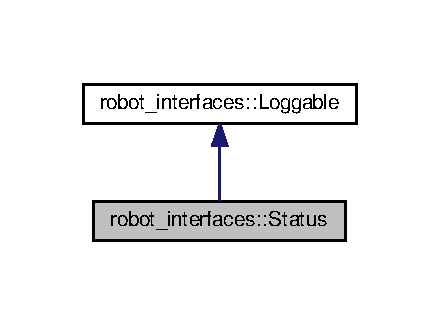
\includegraphics[width=211pt]{structrobot__interfaces_1_1Status__inherit__graph}
\end{center}
\end{figure}


Collaboration diagram for robot\+\_\+interfaces\+:\+:Status\+:
\nopagebreak
\begin{figure}[H]
\begin{center}
\leavevmode
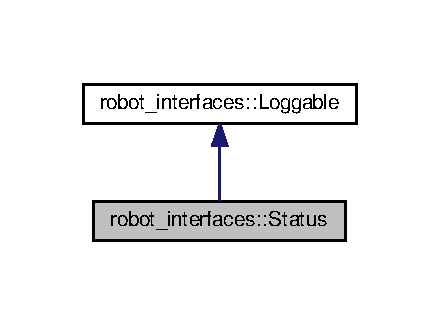
\includegraphics[width=211pt]{structrobot__interfaces_1_1Status__coll__graph}
\end{center}
\end{figure}
\subsection*{Public Types}
\begin{DoxyCompactItemize}
\item 
enum {\bfseries Error\+Status} \{ {\bfseries N\+O\+\_\+\+E\+R\+R\+OR} = 0, 
{\bfseries D\+R\+I\+V\+E\+R\+\_\+\+E\+R\+R\+OR}, 
{\bfseries B\+A\+C\+K\+E\+N\+D\+\_\+\+E\+R\+R\+OR}
 \}\hypertarget{structrobot__interfaces_1_1Status_a88f1cb8387648815ca75754985bdb3b6}{}\label{structrobot__interfaces_1_1Status_a88f1cb8387648815ca75754985bdb3b6}

\end{DoxyCompactItemize}
\subsection*{Public Member Functions}
\begin{DoxyCompactItemize}
\item 
{\footnotesize template$<$class Archive $>$ }\\void {\bfseries serialize} (Archive \&archive)\hypertarget{structrobot__interfaces_1_1Status_a5531f83e2ef30f7629548194b4e3e9da}{}\label{structrobot__interfaces_1_1Status_a5531f83e2ef30f7629548194b4e3e9da}

\item 
std\+::vector$<$ std\+::string $>$ {\bfseries get\+\_\+name} () override\hypertarget{structrobot__interfaces_1_1Status_a2cd6543deb86d878ba43153c18d2fadb}{}\label{structrobot__interfaces_1_1Status_a2cd6543deb86d878ba43153c18d2fadb}

\item 
std\+::vector$<$ std\+::vector$<$ double $>$ $>$ {\bfseries get\+\_\+data} () override\hypertarget{structrobot__interfaces_1_1Status_af530134f33fa21c02d1157636c385fa3}{}\label{structrobot__interfaces_1_1Status_af530134f33fa21c02d1157636c385fa3}

\end{DoxyCompactItemize}
\subsection*{Public Attributes}
\begin{DoxyCompactItemize}
\item 
uint32\+\_\+t \hyperlink{structrobot__interfaces_1_1Status_a8ccb682cd2ba81059991f3b0b9ff0c00}{action\+\_\+repetitions} = 0\hypertarget{structrobot__interfaces_1_1Status_a8ccb682cd2ba81059991f3b0b9ff0c00}{}\label{structrobot__interfaces_1_1Status_a8ccb682cd2ba81059991f3b0b9ff0c00}

\begin{DoxyCompactList}\small\item\em Number of times the current action has been repeated because no new action has been provided. \end{DoxyCompactList}\item 
Error\+Status \hyperlink{structrobot__interfaces_1_1Status_a80ffe66121d425d48386b39984cd4c7b}{error\+\_\+status} = Error\+Status\+::\+N\+O\+\_\+\+E\+R\+R\+OR\hypertarget{structrobot__interfaces_1_1Status_a80ffe66121d425d48386b39984cd4c7b}{}\label{structrobot__interfaces_1_1Status_a80ffe66121d425d48386b39984cd4c7b}

\begin{DoxyCompactList}\small\item\em Indicates if there is an error and, if yes, in which component. \end{DoxyCompactList}\item 
std\+::string \hyperlink{structrobot__interfaces_1_1Status_a7da10fb73cd19f2840c438d321eac744}{error\+\_\+message}
\begin{DoxyCompactList}\small\item\em Message describing the error. \end{DoxyCompactList}\end{DoxyCompactItemize}


\subsection{Detailed Description}
\hyperlink{structrobot__interfaces_1_1Status}{Status} information from the backend. 

This struct is used to report status information that is not directly robot-\/related from the backend to the frontend. 

\subsection{Member Data Documentation}
\index{robot\+\_\+interfaces\+::\+Status@{robot\+\_\+interfaces\+::\+Status}!error\+\_\+message@{error\+\_\+message}}
\index{error\+\_\+message@{error\+\_\+message}!robot\+\_\+interfaces\+::\+Status@{robot\+\_\+interfaces\+::\+Status}}
\subsubsection[{\texorpdfstring{error\+\_\+message}{error_message}}]{\setlength{\rightskip}{0pt plus 5cm}std\+::string robot\+\_\+interfaces\+::\+Status\+::error\+\_\+message}\hypertarget{structrobot__interfaces_1_1Status_a7da10fb73cd19f2840c438d321eac744}{}\label{structrobot__interfaces_1_1Status_a7da10fb73cd19f2840c438d321eac744}


Message describing the error. 

Value is undefined if {\ttfamily error\+\_\+status == N\+O\+\_\+\+E\+R\+R\+OR}. 

The documentation for this struct was generated from the following file\+:\begin{DoxyCompactItemize}
\item 
include/robot\+\_\+interfaces/\hyperlink{status_8hpp}{status.\+hpp}\end{DoxyCompactItemize}

\hypertarget{structrobot__interfaces_1_1TriFingerTypes}{}\section{robot\+\_\+interfaces\+:\+:Tri\+Finger\+Types Struct Reference}
\label{structrobot__interfaces_1_1TriFingerTypes}\index{robot\+\_\+interfaces\+::\+Tri\+Finger\+Types@{robot\+\_\+interfaces\+::\+Tri\+Finger\+Types}}


Types for the Tri\+Finger robot (basically three times the Finger).  




{\ttfamily \#include $<$trifinger\+\_\+types.\+hpp$>$}



Inheritance diagram for robot\+\_\+interfaces\+:\+:Tri\+Finger\+Types\+:
\nopagebreak
\begin{figure}[H]
\begin{center}
\leavevmode
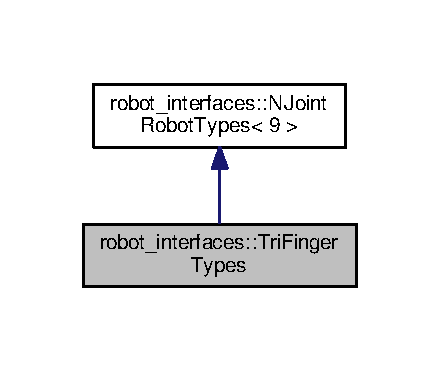
\includegraphics[width=211pt]{structrobot__interfaces_1_1TriFingerTypes__inherit__graph}
\end{center}
\end{figure}


Collaboration diagram for robot\+\_\+interfaces\+:\+:Tri\+Finger\+Types\+:
\nopagebreak
\begin{figure}[H]
\begin{center}
\leavevmode
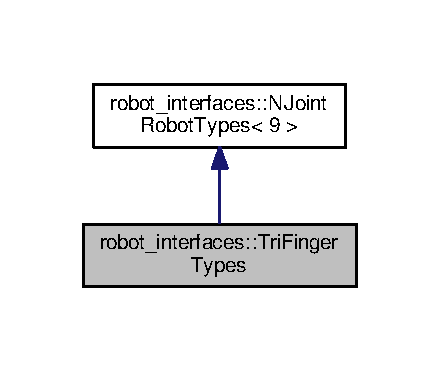
\includegraphics[width=211pt]{structrobot__interfaces_1_1TriFingerTypes__coll__graph}
\end{center}
\end{figure}
\subsection*{Additional Inherited Members}


\subsection{Detailed Description}
Types for the Tri\+Finger robot (basically three times the Finger). 

The documentation for this struct was generated from the following file\+:\begin{DoxyCompactItemize}
\item 
include/robot\+\_\+interfaces/trifinger\+\_\+types.\+hpp\end{DoxyCompactItemize}

\chapter{File Documentation}
\hypertarget{demo_8cpp}{}\section{demos/demo.cpp File Reference}
\label{demo_8cpp}\index{demos/demo.\+cpp@{demos/demo.\+cpp}}


Minimal demo of robot driver, backend and frontend.  


{\ttfamily \#include \char`\"{}robot\+\_\+interfaces/monitored\+\_\+robot\+\_\+driver.\+hpp\char`\"{}}\\*
{\ttfamily \#include \char`\"{}robot\+\_\+interfaces/robot.\+hpp\char`\"{}}\\*
{\ttfamily \#include \char`\"{}robot\+\_\+interfaces/robot\+\_\+backend.\+hpp\char`\"{}}\\*
{\ttfamily \#include \char`\"{}robot\+\_\+interfaces/robot\+\_\+driver.\+hpp\char`\"{}}\\*
{\ttfamily \#include \char`\"{}robot\+\_\+interfaces/robot\+\_\+frontend.\+hpp\char`\"{}}\\*
{\ttfamily \#include \char`\"{}robot\+\_\+interfaces/status.\+hpp\char`\"{}}\\*
{\ttfamily \#include $<$memory$>$}\\*
Include dependency graph for demo.\+cpp\+:
\nopagebreak
\begin{figure}[H]
\begin{center}
\leavevmode
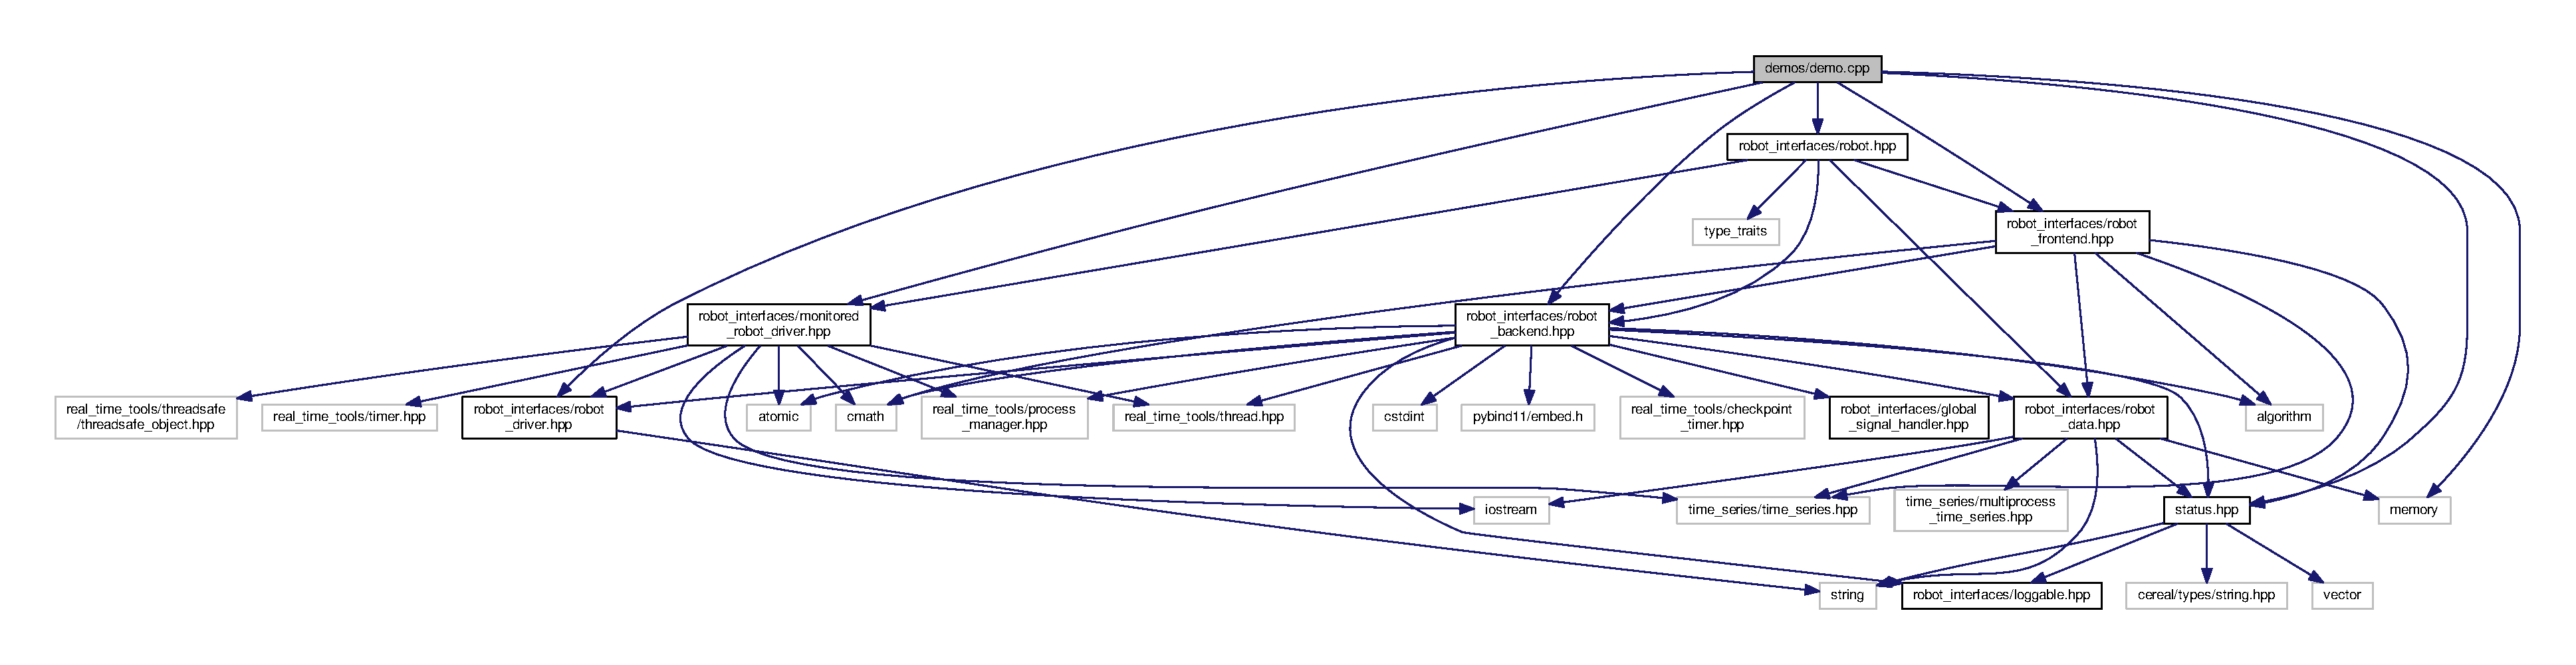
\includegraphics[width=350pt]{demo_8cpp__incl}
\end{center}
\end{figure}
\subsection*{Classes}
\begin{DoxyCompactItemize}
\item 
class \hyperlink{classAction}{Action}
\item 
class \hyperlink{classObservation}{Observation}
\item 
class \hyperlink{classDriver}{Driver}
\end{DoxyCompactItemize}
\subsection*{Functions}
\begin{DoxyCompactItemize}
\item 
int {\bfseries main} ()\hypertarget{demo_8cpp_ae66f6b31b5ad750f1fe042a706a4e3d4}{}\label{demo_8cpp_ae66f6b31b5ad750f1fe042a706a4e3d4}

\end{DoxyCompactItemize}


\subsection{Detailed Description}
Minimal demo of robot driver, backend and frontend. 

\begin{DoxyAuthor}{Author}
Vincent Berenz license License B\+S\+D-\/3-\/\+Clause 
\end{DoxyAuthor}
\begin{DoxyCopyright}{Copyright}
Copyright (c) 2019, Max Planck Gesellschaft. 
\end{DoxyCopyright}

\hypertarget{demo__multiprocess__backend_8cpp}{}\section{demos/demo\+\_\+multiprocess\+\_\+backend.cpp File Reference}
\label{demo__multiprocess__backend_8cpp}\index{demos/demo\+\_\+multiprocess\+\_\+backend.\+cpp@{demos/demo\+\_\+multiprocess\+\_\+backend.\+cpp}}


Minimal demo of robot driver/backend running in its own process.  


{\ttfamily \#include $<$memory$>$}\\*
{\ttfamily \#include \char`\"{}robot\+\_\+interfaces/robot\+\_\+backend.\+hpp\char`\"{}}\\*
{\ttfamily \#include \char`\"{}robot\+\_\+interfaces/robot\+\_\+driver.\+hpp\char`\"{}}\\*
{\ttfamily \#include \char`\"{}types.\+hpp\char`\"{}}\\*
Include dependency graph for demo\+\_\+multiprocess\+\_\+backend.\+cpp\+:
\nopagebreak
\begin{figure}[H]
\begin{center}
\leavevmode
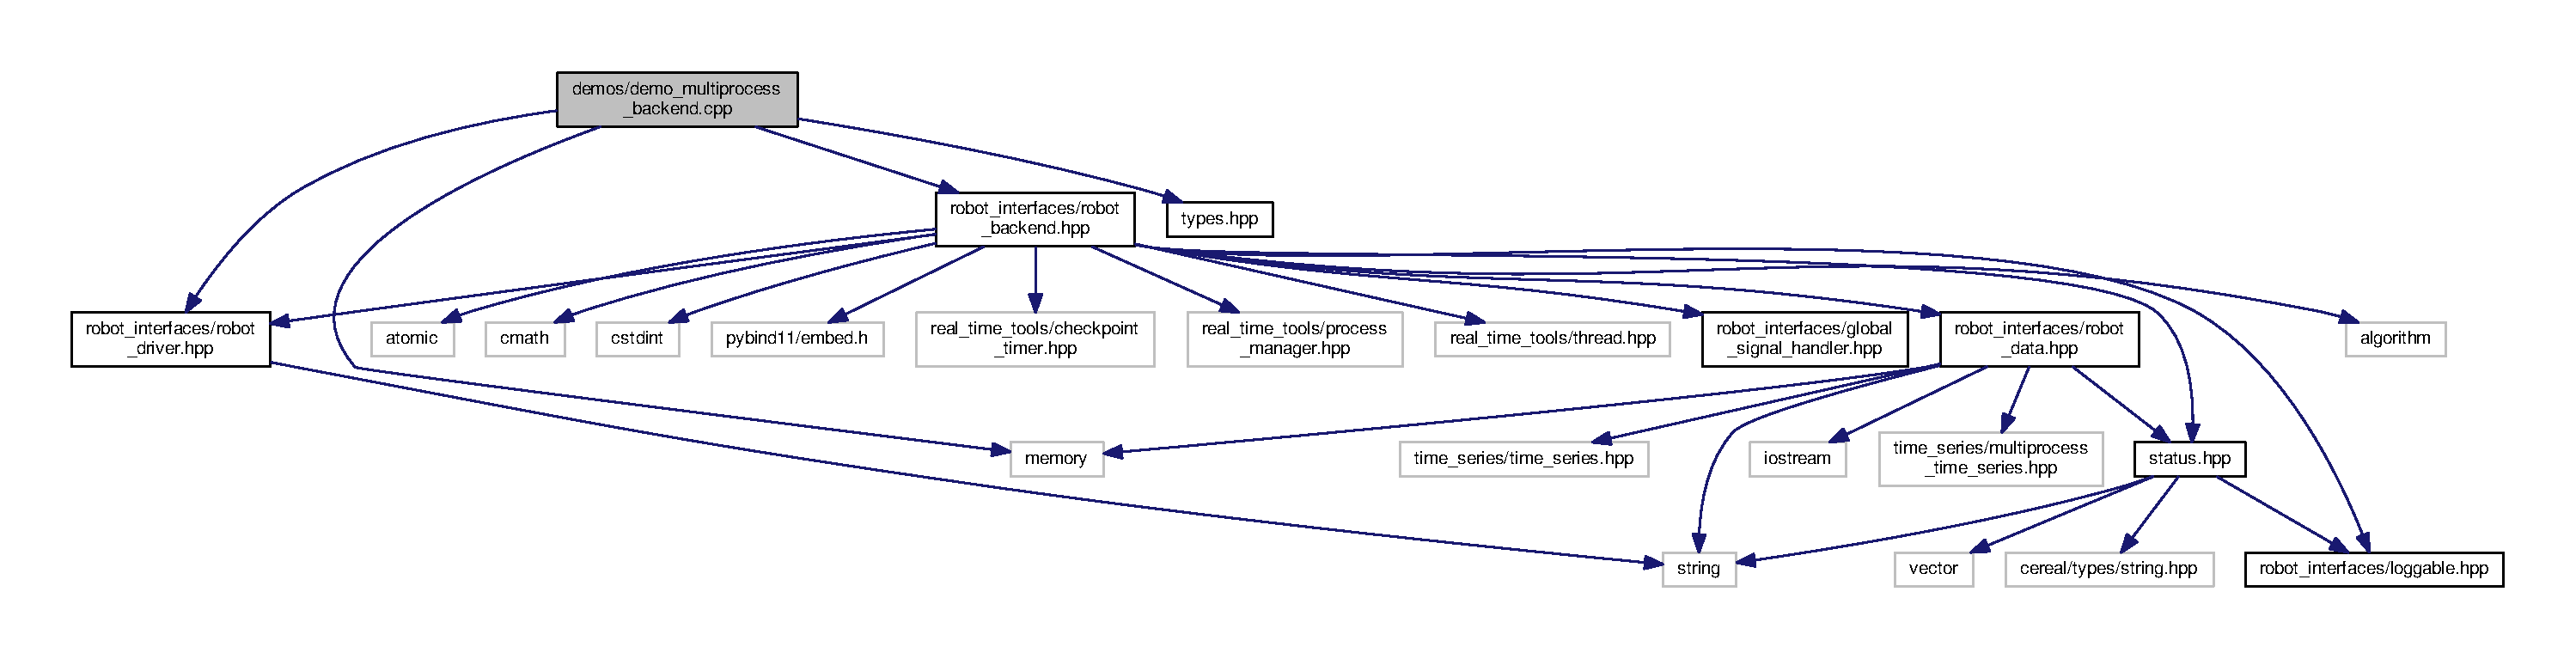
\includegraphics[width=350pt]{demo__multiprocess__backend_8cpp__incl}
\end{center}
\end{figure}
\subsection*{Classes}
\begin{DoxyCompactItemize}
\item 
class \hyperlink{classDriver}{Driver}
\end{DoxyCompactItemize}
\subsection*{Functions}
\begin{DoxyCompactItemize}
\item 
int {\bfseries main} ()\hypertarget{demo__multiprocess__backend_8cpp_ae66f6b31b5ad750f1fe042a706a4e3d4}{}\label{demo__multiprocess__backend_8cpp_ae66f6b31b5ad750f1fe042a706a4e3d4}

\end{DoxyCompactItemize}


\subsection{Detailed Description}
Minimal demo of robot driver/backend running in its own process. 

\begin{DoxyAuthor}{Author}
Vincent Berenz, Felix Widmaier license License B\+S\+D-\/3-\/\+Clause 
\end{DoxyAuthor}
\begin{DoxyCopyright}{Copyright}
Copyright (c) 2019-\/2020, Max Planck Gesellschaft. 
\end{DoxyCopyright}

\hypertarget{demo__multiprocess__frontend_8cpp}{}\section{demos/demo\+\_\+multiprocess\+\_\+frontend.cpp File Reference}
\label{demo__multiprocess__frontend_8cpp}\index{demos/demo\+\_\+multiprocess\+\_\+frontend.\+cpp@{demos/demo\+\_\+multiprocess\+\_\+frontend.\+cpp}}


Minimal demo of robot frontend running in its own process.  


{\ttfamily \#include $<$memory$>$}\\*
{\ttfamily \#include \char`\"{}robot\+\_\+interfaces/robot\+\_\+frontend.\+hpp\char`\"{}}\\*
{\ttfamily \#include \char`\"{}types.\+hpp\char`\"{}}\\*
Include dependency graph for demo\+\_\+multiprocess\+\_\+frontend.\+cpp\+:
\nopagebreak
\begin{figure}[H]
\begin{center}
\leavevmode
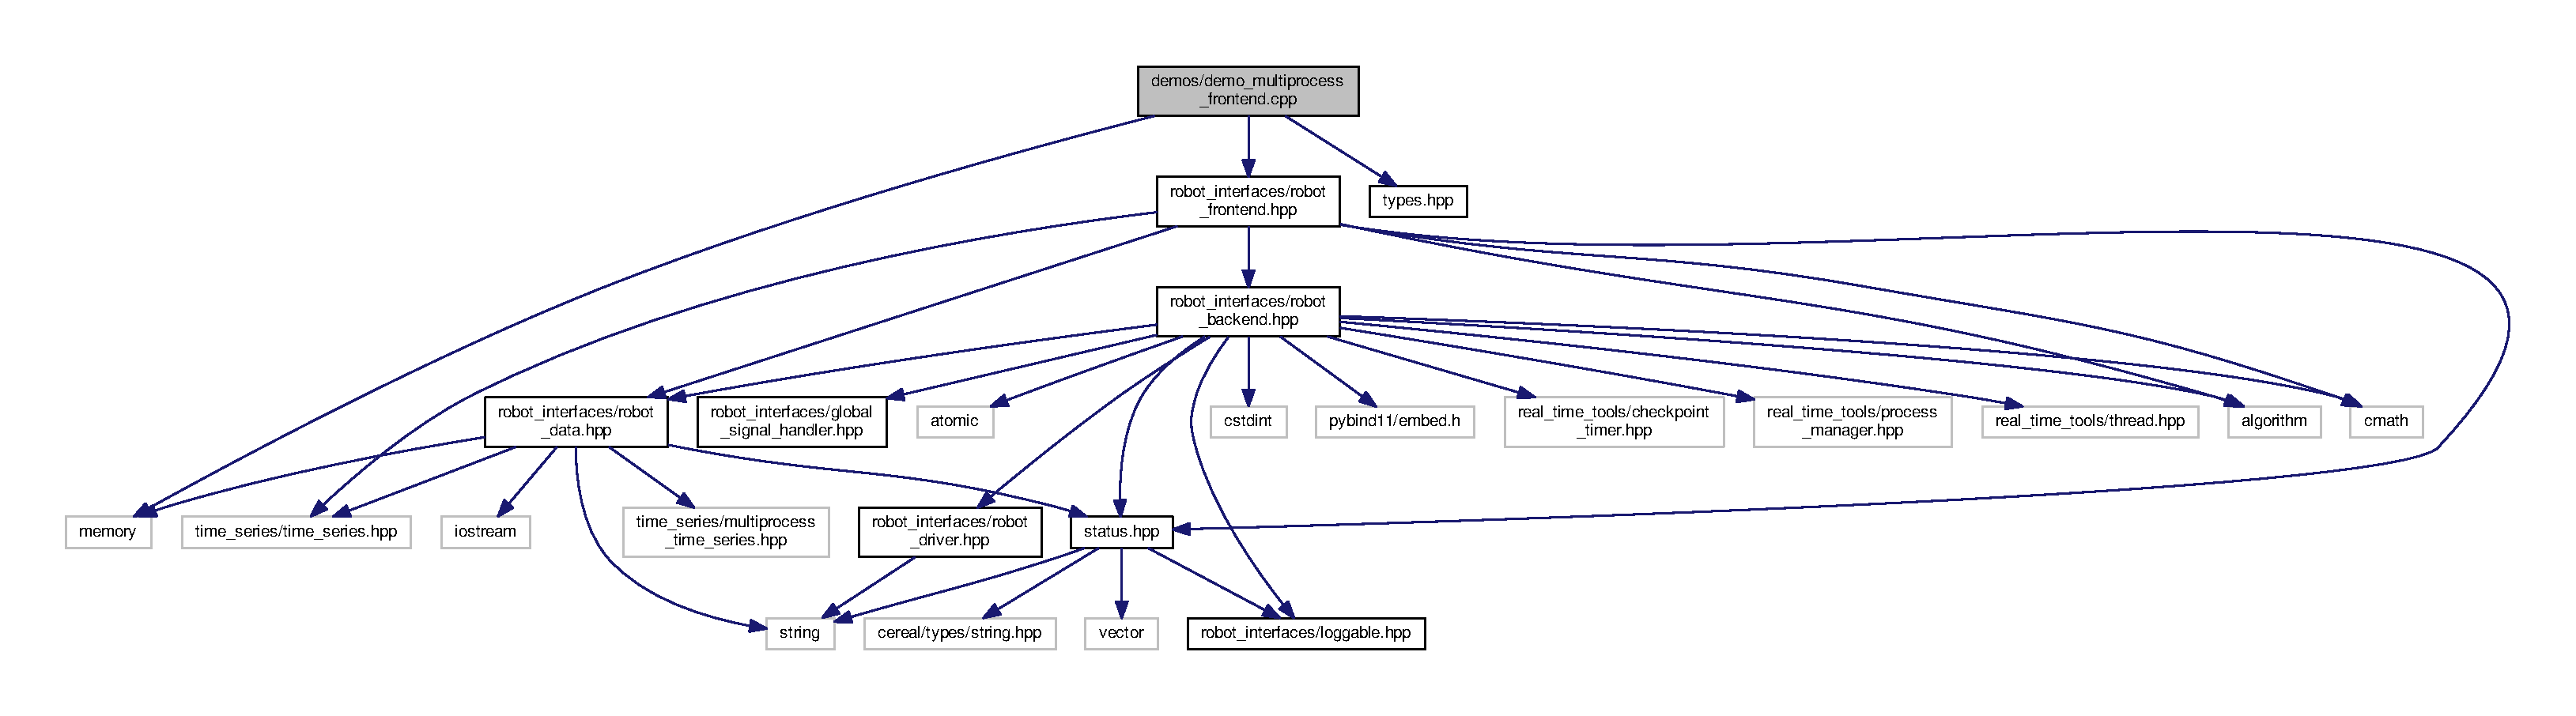
\includegraphics[width=350pt]{demo__multiprocess__frontend_8cpp__incl}
\end{center}
\end{figure}
\subsection*{Functions}
\begin{DoxyCompactItemize}
\item 
int {\bfseries main} ()\hypertarget{demo__multiprocess__frontend_8cpp_ae66f6b31b5ad750f1fe042a706a4e3d4}{}\label{demo__multiprocess__frontend_8cpp_ae66f6b31b5ad750f1fe042a706a4e3d4}

\end{DoxyCompactItemize}


\subsection{Detailed Description}
Minimal demo of robot frontend running in its own process. 

\begin{DoxyAuthor}{Author}
Vincent Berenz, Felix Widmaier license License B\+S\+D-\/3-\/\+Clause 
\end{DoxyAuthor}
\begin{DoxyCopyright}{Copyright}
Copyright (c) 2019-\/2020, Max Planck Gesellschaft. 
\end{DoxyCopyright}

\hypertarget{types_8hpp}{}\section{demos/types.hpp File Reference}
\label{types_8hpp}\index{demos/types.\+hpp@{demos/types.\+hpp}}


license License B\+S\+D-\/3-\/\+Clause  


This graph shows which files directly or indirectly include this file\+:
\nopagebreak
\begin{figure}[H]
\begin{center}
\leavevmode
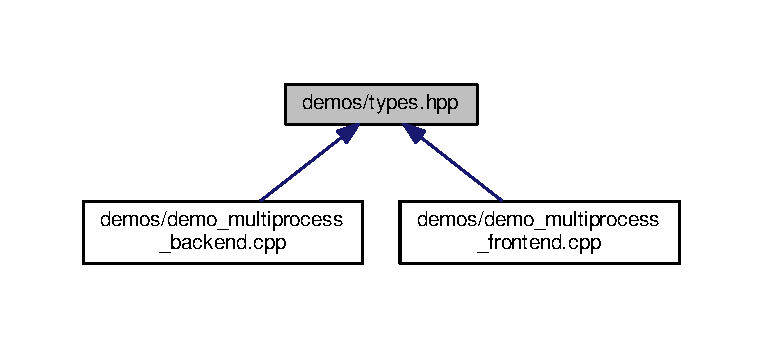
\includegraphics[width=350pt]{types_8hpp__dep__incl}
\end{center}
\end{figure}
\subsection*{Classes}
\begin{DoxyCompactItemize}
\item 
class \hyperlink{classrobot__interfaces_1_1demo_1_1Action}{robot\+\_\+interfaces\+::demo\+::\+Action}
\begin{DoxyCompactList}\small\item\em Actions to be performed by robot, will be received by \hyperlink{classDriver}{Driver}. \end{DoxyCompactList}\item 
class \hyperlink{classrobot__interfaces_1_1demo_1_1Observation}{robot\+\_\+interfaces\+::demo\+::\+Observation}
\begin{DoxyCompactList}\small\item\em Read from the robot by \hyperlink{classDriver}{Driver}. \end{DoxyCompactList}\end{DoxyCompactItemize}


\subsection{Detailed Description}
license License B\+S\+D-\/3-\/\+Clause 

\begin{DoxyCopyright}{Copyright}
Copyright (c) 2019-\/2020, Max Planck Gesellschaft.
\end{DoxyCopyright}
Simple \hyperlink{classAction}{Action} and \hyperlink{classObservation}{Observation} types that are used by some demos. 
\hypertarget{cereal__eigen_8hpp}{}\section{include/robot\+\_\+interfaces/cereal\+\_\+eigen.hpp File Reference}
\label{cereal__eigen_8hpp}\index{include/robot\+\_\+interfaces/cereal\+\_\+eigen.\+hpp@{include/robot\+\_\+interfaces/cereal\+\_\+eigen.\+hpp}}


Serialization functions for serializing Eigen matrices and arrays with cereal.  


{\ttfamily \#include $<$Eigen/\+Eigen$>$}\\*
{\ttfamily \#include $<$type\+\_\+traits$>$}\\*
Include dependency graph for cereal\+\_\+eigen.\+hpp\+:
\nopagebreak
\begin{figure}[H]
\begin{center}
\leavevmode
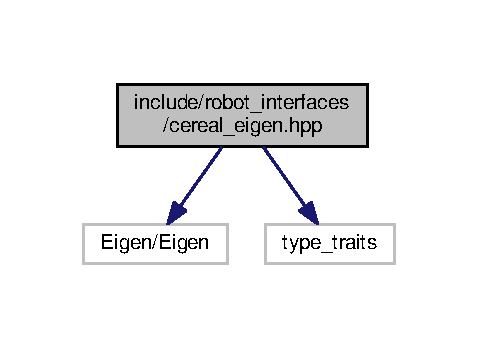
\includegraphics[width=230pt]{cereal__eigen_8hpp__incl}
\end{center}
\end{figure}
This graph shows which files directly or indirectly include this file\+:
\nopagebreak
\begin{figure}[H]
\begin{center}
\leavevmode
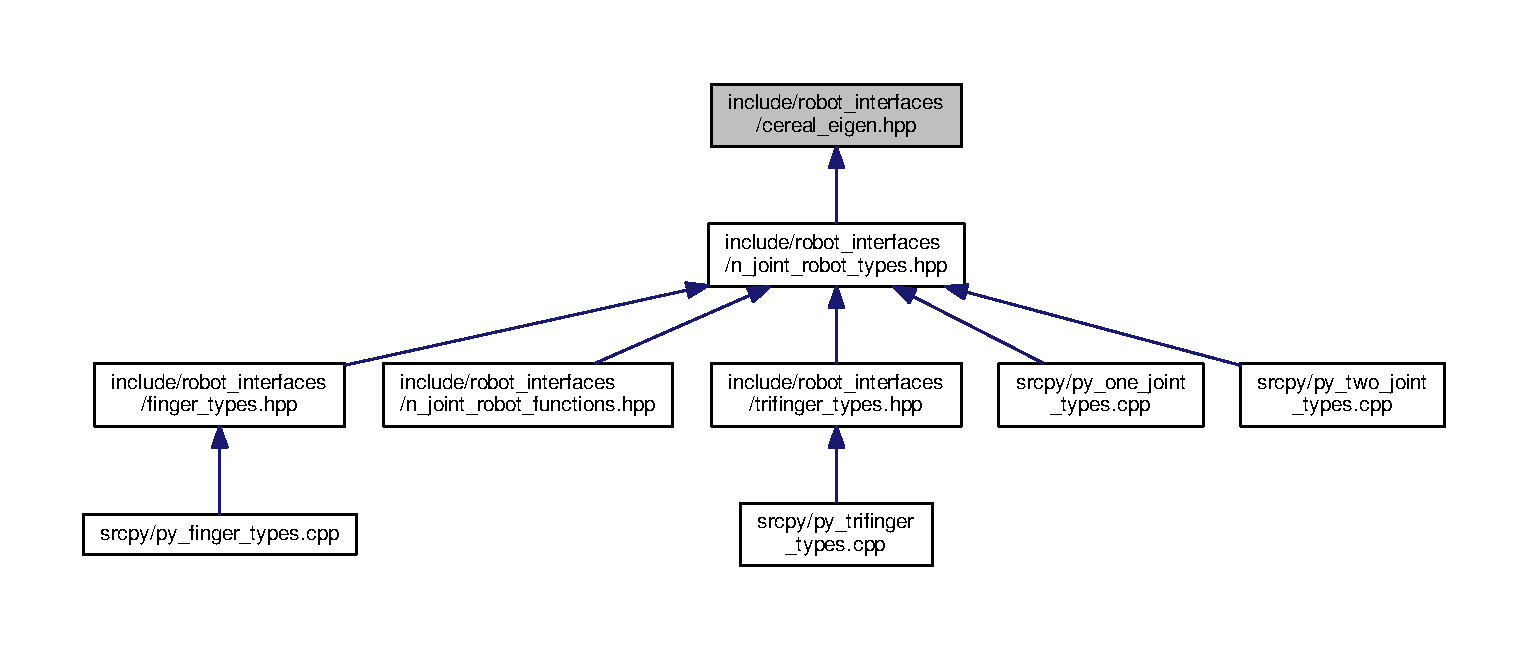
\includegraphics[width=350pt]{cereal__eigen_8hpp__dep__incl}
\end{center}
\end{figure}
\subsection*{Functions}
\begin{DoxyCompactItemize}
\item 
{\footnotesize template$<$class Archive , class Derived $>$ }\\std\+::enable\+\_\+if$<$ traits\+::is\+\_\+output\+\_\+serializable$<$ Binary\+Data$<$ typename Derived\+::\+Scalar $>$, Archive $>$\+::value, void $>$\+::type {\bfseries cereal\+::save} (Archive \&archive, const Eigen\+::\+Plain\+Object\+Base$<$ Derived $>$ \&object)\hypertarget{cereal__eigen_8hpp_aba6cfc68d144d36a4ac46cdaa4f9626c}{}\label{cereal__eigen_8hpp_aba6cfc68d144d36a4ac46cdaa4f9626c}

\item 
{\footnotesize template$<$class Archive , class Derived $>$ }\\std\+::enable\+\_\+if$<$ traits\+::is\+\_\+input\+\_\+serializable$<$ Binary\+Data$<$ typename Derived\+::\+Scalar $>$, Archive $>$\+::value, void $>$\+::type {\bfseries cereal\+::load} (Archive \&archive, Eigen\+::\+Plain\+Object\+Base$<$ Derived $>$ \&object)\hypertarget{cereal__eigen_8hpp_a2c410cde64d019622dd6d81387316eaa}{}\label{cereal__eigen_8hpp_a2c410cde64d019622dd6d81387316eaa}

\end{DoxyCompactItemize}


\subsection{Detailed Description}
Serialization functions for serializing Eigen matrices and arrays with cereal. 

\begin{DoxyAuthor}{Authors}
Azoth, eudoxos 
\end{DoxyAuthor}
\begin{DoxyDate}{Date}
2020-\/01-\/15 
\end{DoxyDate}
\begin{DoxyRefDesc}{License}
\item[\hyperlink{license__license000001}{License}]CC B\+Y-\/\+SA 4.\+0 \end{DoxyRefDesc}
\begin{DoxyRefDesc}{Todo}
\item[\hyperlink{todo__todo000001}{Todo}]Move this to some \char`\"{}serialization tools\char`\"{} package.\end{DoxyRefDesc}


Taken from \href{https://stackoverflow.com/a/51944389/2095383}{\tt https\+://stackoverflow.\+com/a/51944389/2095383} with minor modifications. 
\hypertarget{global__signal__handler_8hpp}{}\section{include/robot\+\_\+interfaces/global\+\_\+signal\+\_\+handler.hpp File Reference}
\label{global__signal__handler_8hpp}\index{include/robot\+\_\+interfaces/global\+\_\+signal\+\_\+handler.\+hpp@{include/robot\+\_\+interfaces/global\+\_\+signal\+\_\+handler.\+hpp}}
This graph shows which files directly or indirectly include this file\+:
\nopagebreak
\begin{figure}[H]
\begin{center}
\leavevmode
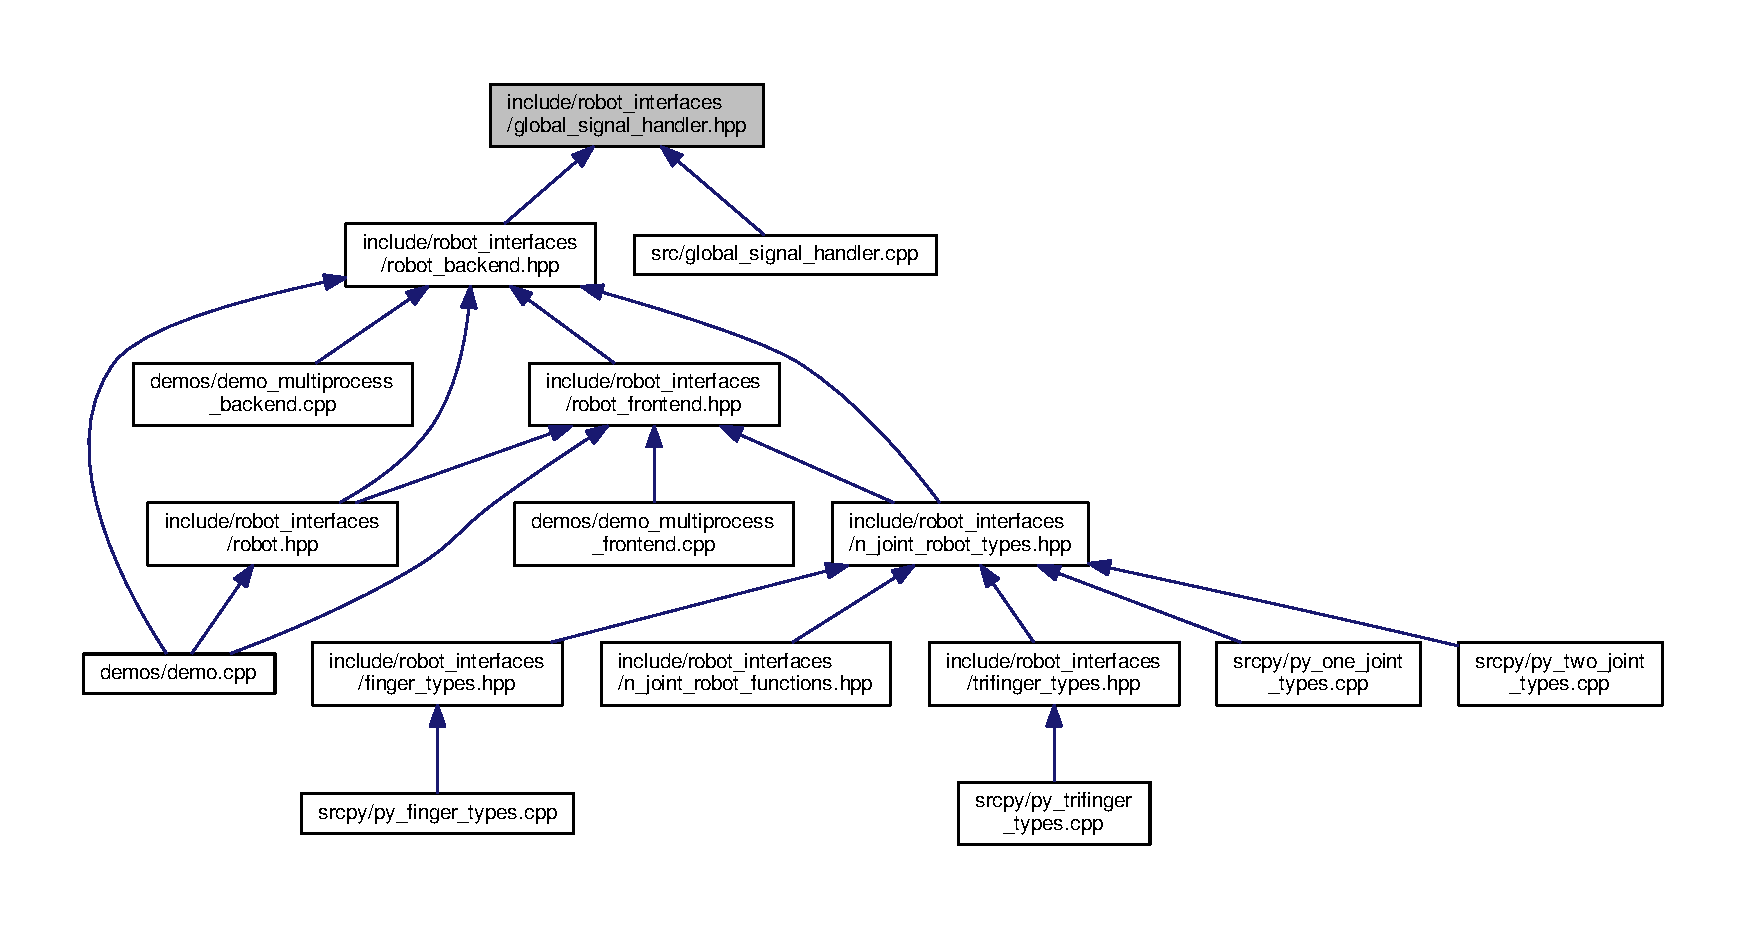
\includegraphics[width=350pt]{global__signal__handler_8hpp__dep__incl}
\end{center}
\end{figure}
\subsection*{Classes}
\begin{DoxyCompactItemize}
\item 
class \hyperlink{classrobot__interfaces_1_1GlobalSignalHandler}{robot\+\_\+interfaces\+::\+Global\+Signal\+Handler}
\begin{DoxyCompactList}\small\item\em Static class implementing a signal handler and providing information about S\+I\+G\+I\+NT. \end{DoxyCompactList}\end{DoxyCompactItemize}


\subsection{Detailed Description}
\begin{DoxyCopyright}{Copyright}
2020, New York University, Max Planck Gesellschaft. All rights reserved. 
\end{DoxyCopyright}
\begin{DoxyRefDesc}{License}
\item[\hyperlink{license__license000002}{License}]B\+SD 3-\/clause \end{DoxyRefDesc}

\hypertarget{pybind__helper_8hpp}{}\section{include/robot\+\_\+interfaces/pybind\+\_\+helper.hpp File Reference}
\label{pybind__helper_8hpp}\index{include/robot\+\_\+interfaces/pybind\+\_\+helper.\+hpp@{include/robot\+\_\+interfaces/pybind\+\_\+helper.\+hpp}}


Helper functions for creating Python bindings.  


{\ttfamily \#include $<$pybind11/eigen.\+h$>$}\\*
{\ttfamily \#include $<$pybind11/pybind11.\+h$>$}\\*
{\ttfamily \#include $<$pybind11/stl\+\_\+bind.\+h$>$}\\*
Include dependency graph for pybind\+\_\+helper.\+hpp\+:
\nopagebreak
\begin{figure}[H]
\begin{center}
\leavevmode
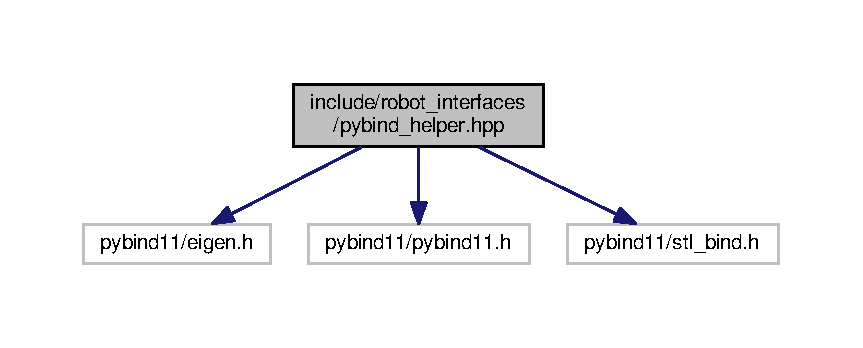
\includegraphics[width=350pt]{pybind__helper_8hpp__incl}
\end{center}
\end{figure}
This graph shows which files directly or indirectly include this file\+:
\nopagebreak
\begin{figure}[H]
\begin{center}
\leavevmode
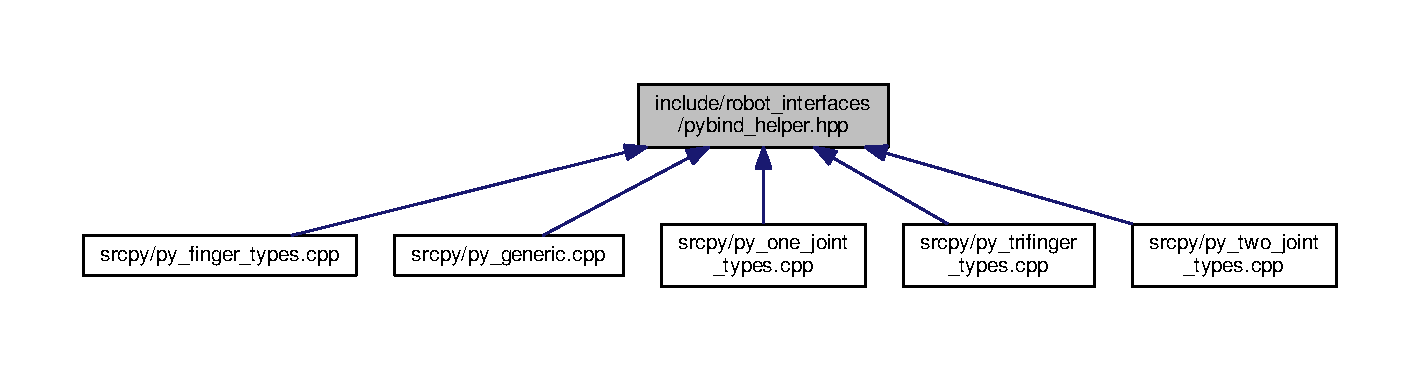
\includegraphics[width=350pt]{pybind__helper_8hpp__dep__incl}
\end{center}
\end{figure}
\subsection*{Functions}
\begin{DoxyCompactItemize}
\item 
{\footnotesize template$<$typename Types $>$ }\\void \hyperlink{pybind__helper_8hpp_a82052567130c3000eeef9f5520885233}{robot\+\_\+interfaces\+::create\+\_\+python\+\_\+bindings} (pybind11\+::module \&m)
\begin{DoxyCompactList}\small\item\em Create Python bindings for the specified robot Types. \end{DoxyCompactList}\end{DoxyCompactItemize}


\subsection{Detailed Description}
Helper functions for creating Python bindings. 



\subsection{Function Documentation}
\index{pybind\+\_\+helper.\+hpp@{pybind\+\_\+helper.\+hpp}!create\+\_\+python\+\_\+bindings@{create\+\_\+python\+\_\+bindings}}
\index{create\+\_\+python\+\_\+bindings@{create\+\_\+python\+\_\+bindings}!pybind\+\_\+helper.\+hpp@{pybind\+\_\+helper.\+hpp}}
\subsubsection[{\texorpdfstring{create\+\_\+python\+\_\+bindings(pybind11\+::module \&m)}{create_python_bindings(pybind11::module &m)}}]{\setlength{\rightskip}{0pt plus 5cm}template$<$typename Types $>$ void robot\+\_\+interfaces\+::create\+\_\+python\+\_\+bindings (
\begin{DoxyParamCaption}
\item[{pybind11\+::module \&}]{m}
\end{DoxyParamCaption}
)}\hypertarget{pybind__helper_8hpp_file_a82052567130c3000eeef9f5520885233}{}\label{pybind__helper_8hpp_file_a82052567130c3000eeef9f5520885233}


Create Python bindings for the specified robot Types. 

With this function, Python bindings can easily be created for new robots that are based on the \hyperlink{structrobot__interfaces_1_1NJointRobotTypes}{N\+Joint\+Robot\+Types}. Example\+: \begin{DoxyVerb}PYBIND11_MODULE(py_fortytwo_types, m)
{
    create_python_bindings<NJointRobotTypes<42>>(m);
}
\end{DoxyVerb}



\begin{DoxyTemplParams}{Template Parameters}
{\em Types} & An instance of \hyperlink{structrobot__interfaces_1_1NJointRobotTypes}{N\+Joint\+Robot\+Types}. \\
\hline
\end{DoxyTemplParams}

\begin{DoxyParams}{Parameters}
{\em m} & The second argument of the P\+Y\+B\+I\+N\+D11\+\_\+\+M\+O\+D\+U\+LE macro. \\
\hline
\end{DoxyParams}

\hypertarget{robot__data_8hpp}{}\section{include/robot\+\_\+interfaces/robot\+\_\+data.hpp File Reference}
\label{robot__data_8hpp}\index{include/robot\+\_\+interfaces/robot\+\_\+data.\+hpp@{include/robot\+\_\+interfaces/robot\+\_\+data.\+hpp}}


Robot\+Data classes for both single-\/ and multi-\/process applications.  


{\ttfamily \#include $<$iostream$>$}\\*
{\ttfamily \#include $<$memory$>$}\\*
{\ttfamily \#include $<$string$>$}\\*
{\ttfamily \#include $<$time\+\_\+series/multiprocess\+\_\+time\+\_\+series.\+hpp$>$}\\*
{\ttfamily \#include $<$time\+\_\+series/time\+\_\+series.\+hpp$>$}\\*
{\ttfamily \#include \char`\"{}status.\+hpp\char`\"{}}\\*
Include dependency graph for robot\+\_\+data.\+hpp\+:
\nopagebreak
\begin{figure}[H]
\begin{center}
\leavevmode
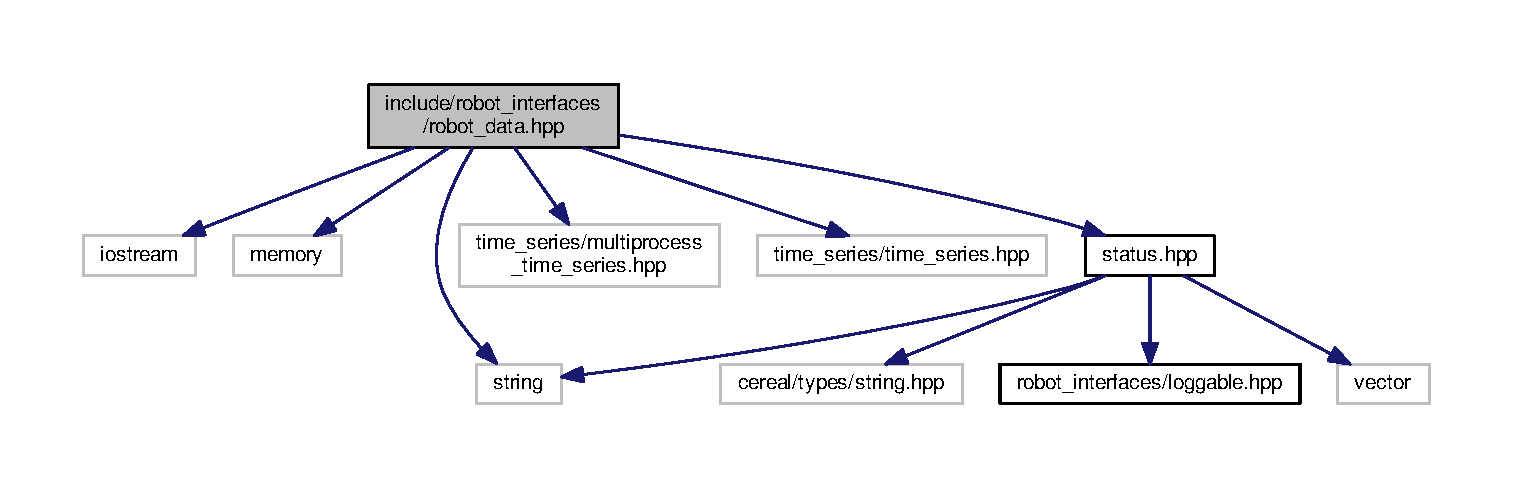
\includegraphics[width=350pt]{robot__data_8hpp__incl}
\end{center}
\end{figure}
This graph shows which files directly or indirectly include this file\+:
\nopagebreak
\begin{figure}[H]
\begin{center}
\leavevmode
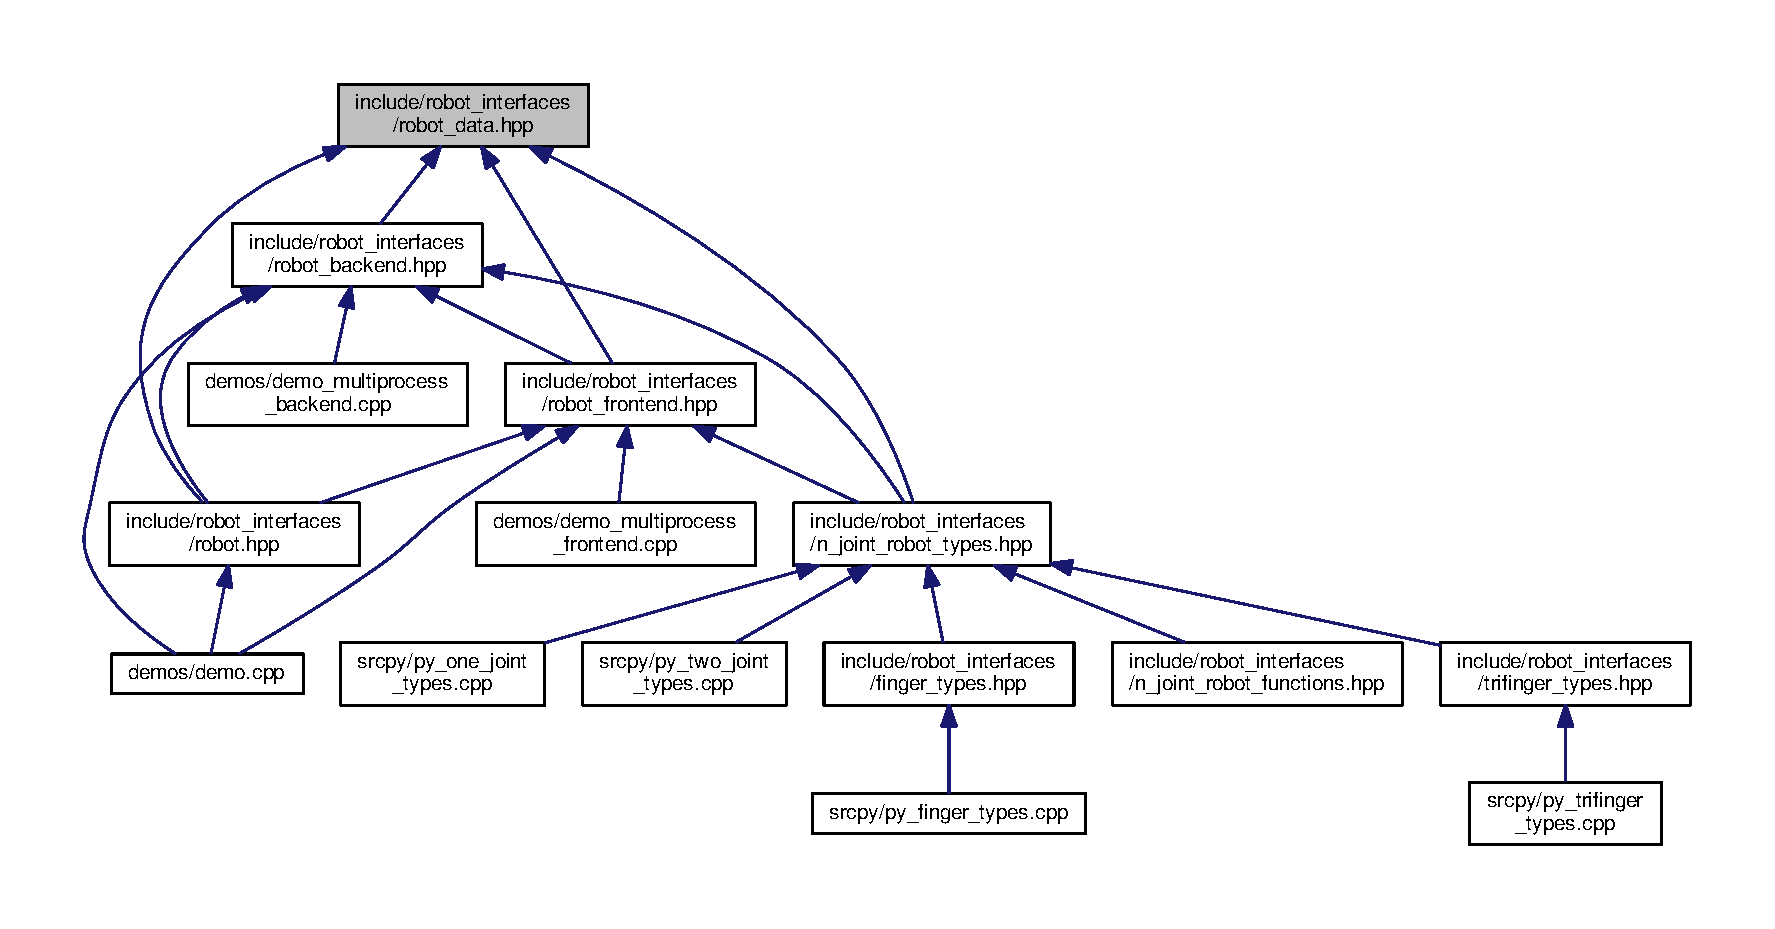
\includegraphics[width=350pt]{robot__data_8hpp__dep__incl}
\end{center}
\end{figure}
\subsection*{Classes}
\begin{DoxyCompactItemize}
\item 
class \hyperlink{classrobot__interfaces_1_1RobotData}{robot\+\_\+interfaces\+::\+Robot\+Data$<$ Action, Observation $>$}
\begin{DoxyCompactList}\small\item\em Contains all the input and output data of the robot. \end{DoxyCompactList}\item 
class \hyperlink{classrobot__interfaces_1_1SingleProcessRobotData}{robot\+\_\+interfaces\+::\+Single\+Process\+Robot\+Data$<$ Action, Observation $>$}
\begin{DoxyCompactList}\small\item\em \hyperlink{classrobot__interfaces_1_1RobotData}{Robot\+Data} instance using single process time series. \end{DoxyCompactList}\item 
class \hyperlink{classrobot__interfaces_1_1MultiProcessRobotData}{robot\+\_\+interfaces\+::\+Multi\+Process\+Robot\+Data$<$ Action, Observation $>$}
\begin{DoxyCompactList}\small\item\em \hyperlink{classrobot__interfaces_1_1RobotData}{Robot\+Data} instance using multi process time series. \end{DoxyCompactList}\end{DoxyCompactItemize}


\subsection{Detailed Description}
Robot\+Data classes for both single-\/ and multi-\/process applications. 

\begin{DoxyRefDesc}{License}
\item[\hyperlink{license__license000003}{License}]B\+SD 3-\/clause \end{DoxyRefDesc}
\begin{DoxyCopyright}{Copyright}
Copyright (c) 2018-\/2020, New York University and Max Planck Gesellschaft 
\end{DoxyCopyright}

\hypertarget{pybind__sensors_8hpp}{}\section{include/robot\+\_\+interfaces/sensors/pybind\+\_\+sensors.hpp File Reference}
\label{pybind__sensors_8hpp}\index{include/robot\+\_\+interfaces/sensors/pybind\+\_\+sensors.\+hpp@{include/robot\+\_\+interfaces/sensors/pybind\+\_\+sensors.\+hpp}}


Binds methods and objects to enable access from python.  


{\ttfamily \#include $<$pybind11/eigen.\+h$>$}\\*
{\ttfamily \#include $<$pybind11/pybind11.\+h$>$}\\*
{\ttfamily \#include $<$pybind11/stl.\+h$>$}\\*
{\ttfamily \#include $<$robot\+\_\+interfaces/sensors/sensor\+\_\+backend.\+hpp$>$}\\*
{\ttfamily \#include $<$robot\+\_\+interfaces/sensors/sensor\+\_\+data.\+hpp$>$}\\*
{\ttfamily \#include $<$robot\+\_\+interfaces/sensors/sensor\+\_\+driver.\+hpp$>$}\\*
{\ttfamily \#include $<$robot\+\_\+interfaces/sensors/sensor\+\_\+frontend.\+hpp$>$}\\*
Include dependency graph for pybind\+\_\+sensors.\+hpp\+:
\nopagebreak
\begin{figure}[H]
\begin{center}
\leavevmode
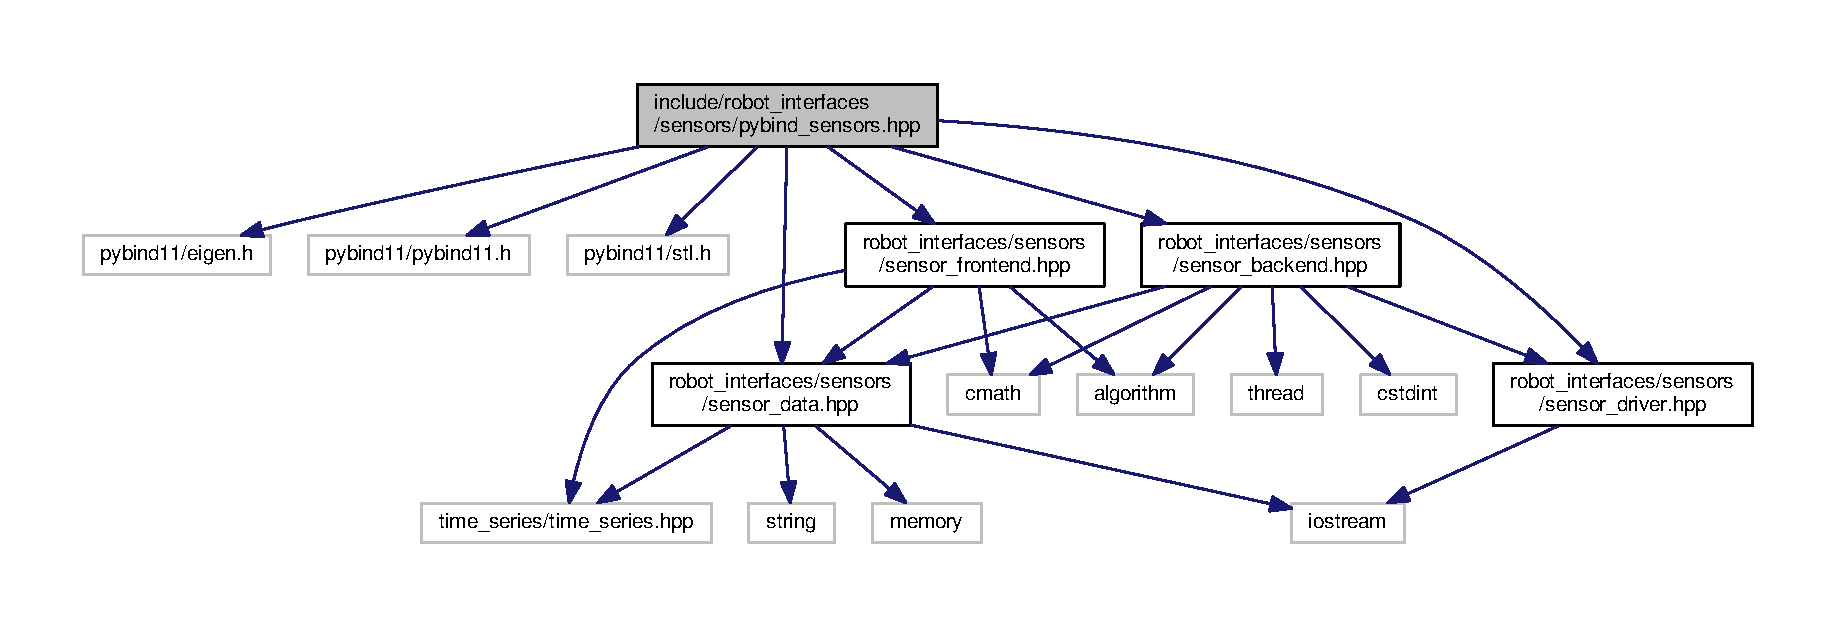
\includegraphics[width=350pt]{pybind__sensors_8hpp__incl}
\end{center}
\end{figure}
\subsection*{Functions}
\begin{DoxyCompactItemize}
\item 
{\footnotesize template$<$typename Observation\+Type $>$ }\\void \hyperlink{pybind__sensors_8hpp_a31fc2ebe96b63e949a14f3f08cfea9b4}{robot\+\_\+interfaces\+::create\+\_\+sensor\+\_\+bindings} (pybind11\+::module \&m)
\begin{DoxyCompactList}\small\item\em Create python bindings for different sensor types. \end{DoxyCompactList}\end{DoxyCompactItemize}


\subsection{Detailed Description}
Binds methods and objects to enable access from python. 

\begin{DoxyCopyright}{Copyright}
2020, New York University, Max Planck Gesellschaft. All rights reserved. 
\end{DoxyCopyright}
\begin{DoxyRefDesc}{License}
\item[\hyperlink{license__license000004}{License}]B\+SD 3-\/clause \end{DoxyRefDesc}


\subsection{Function Documentation}
\index{pybind\+\_\+sensors.\+hpp@{pybind\+\_\+sensors.\+hpp}!create\+\_\+sensor\+\_\+bindings@{create\+\_\+sensor\+\_\+bindings}}
\index{create\+\_\+sensor\+\_\+bindings@{create\+\_\+sensor\+\_\+bindings}!pybind\+\_\+sensors.\+hpp@{pybind\+\_\+sensors.\+hpp}}
\subsubsection[{\texorpdfstring{create\+\_\+sensor\+\_\+bindings(pybind11\+::module \&m)}{create_sensor_bindings(pybind11::module &m)}}]{\setlength{\rightskip}{0pt plus 5cm}template$<$typename Observation\+Type $>$ void robot\+\_\+interfaces\+::create\+\_\+sensor\+\_\+bindings (
\begin{DoxyParamCaption}
\item[{pybind11\+::module \&}]{m}
\end{DoxyParamCaption}
)}\hypertarget{pybind__sensors_8hpp_file_a31fc2ebe96b63e949a14f3f08cfea9b4}{}\label{pybind__sensors_8hpp_file_a31fc2ebe96b63e949a14f3f08cfea9b4}


Create python bindings for different sensor types. 


\begin{DoxyTemplParams}{Template Parameters}
{\em The} & Observation\+Type \\
\hline
\end{DoxyTemplParams}

\hypertarget{sensor__backend_8hpp}{}\section{include/robot\+\_\+interfaces/sensors/sensor\+\_\+backend.hpp File Reference}
\label{sensor__backend_8hpp}\index{include/robot\+\_\+interfaces/sensors/sensor\+\_\+backend.\+hpp@{include/robot\+\_\+interfaces/sensors/sensor\+\_\+backend.\+hpp}}


Connects the driver with sensor data.  


{\ttfamily \#include $<$algorithm$>$}\\*
{\ttfamily \#include $<$cmath$>$}\\*
{\ttfamily \#include $<$cstdint$>$}\\*
{\ttfamily \#include $<$thread$>$}\\*
{\ttfamily \#include $<$robot\+\_\+interfaces/sensors/sensor\+\_\+data.\+hpp$>$}\\*
{\ttfamily \#include $<$robot\+\_\+interfaces/sensors/sensor\+\_\+driver.\+hpp$>$}\\*
Include dependency graph for sensor\+\_\+backend.\+hpp\+:
\nopagebreak
\begin{figure}[H]
\begin{center}
\leavevmode
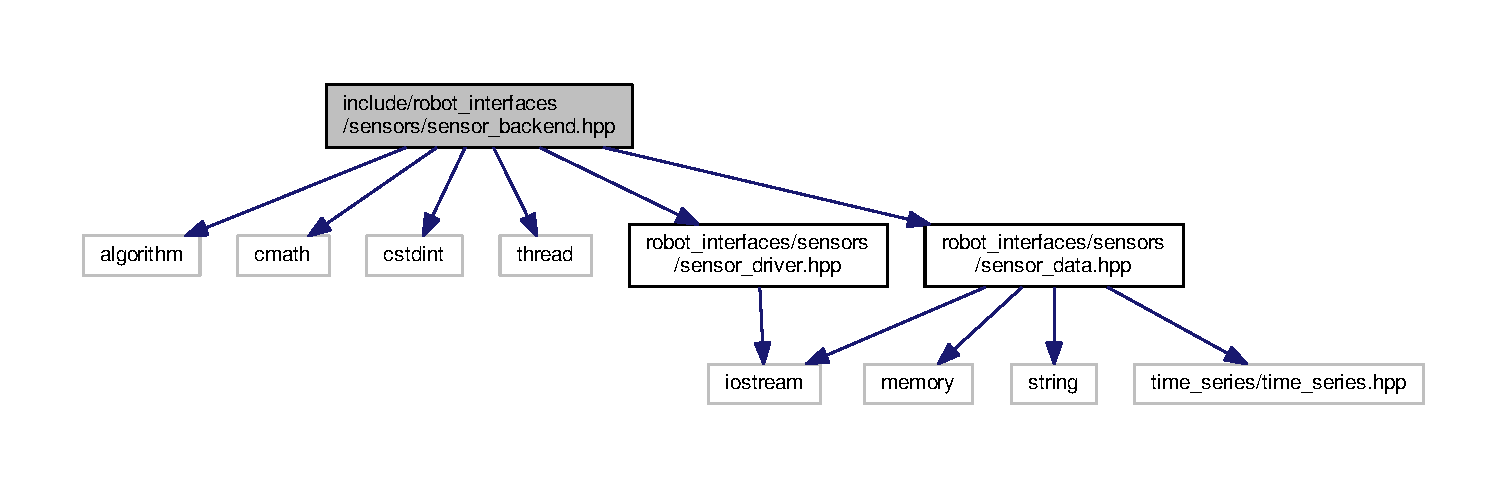
\includegraphics[width=350pt]{sensor__backend_8hpp__incl}
\end{center}
\end{figure}
This graph shows which files directly or indirectly include this file\+:
\nopagebreak
\begin{figure}[H]
\begin{center}
\leavevmode
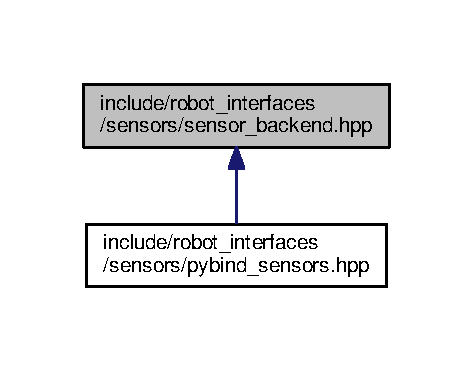
\includegraphics[width=227pt]{sensor__backend_8hpp__dep__incl}
\end{center}
\end{figure}
\subsection*{Classes}
\begin{DoxyCompactItemize}
\item 
class \hyperlink{classrobot__interfaces_1_1SensorBackend}{robot\+\_\+interfaces\+::\+Sensor\+Backend$<$ Observation\+Type $>$}
\begin{DoxyCompactList}\small\item\em Communication link between \hyperlink{classrobot__interfaces_1_1SensorData}{Sensor\+Data} and \hyperlink{classrobot__interfaces_1_1SensorDriver}{Sensor\+Driver}. \end{DoxyCompactList}\end{DoxyCompactItemize}


\subsection{Detailed Description}
Connects the driver with sensor data. 

\begin{DoxyCopyright}{Copyright}
2020, New York University, Max Planck Gesellschaft. All rights reserved. 
\end{DoxyCopyright}
\begin{DoxyRefDesc}{License}
\item[\hyperlink{license__license000005}{License}]B\+SD 3-\/clause \end{DoxyRefDesc}

\hypertarget{sensor__data_8hpp}{}\section{include/robot\+\_\+interfaces/sensors/sensor\+\_\+data.hpp File Reference}
\label{sensor__data_8hpp}\index{include/robot\+\_\+interfaces/sensors/sensor\+\_\+data.\+hpp@{include/robot\+\_\+interfaces/sensors/sensor\+\_\+data.\+hpp}}


To store all the data from all the sensors in use.  


{\ttfamily \#include $<$iostream$>$}\\*
{\ttfamily \#include $<$memory$>$}\\*
{\ttfamily \#include $<$string$>$}\\*
{\ttfamily \#include $<$time\+\_\+series/time\+\_\+series.\+hpp$>$}\\*
Include dependency graph for sensor\+\_\+data.\+hpp\+:
\nopagebreak
\begin{figure}[H]
\begin{center}
\leavevmode
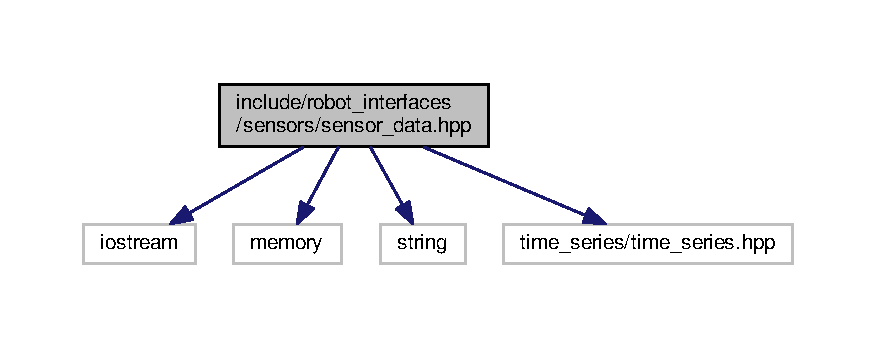
\includegraphics[width=350pt]{sensor__data_8hpp__incl}
\end{center}
\end{figure}
This graph shows which files directly or indirectly include this file\+:
\nopagebreak
\begin{figure}[H]
\begin{center}
\leavevmode
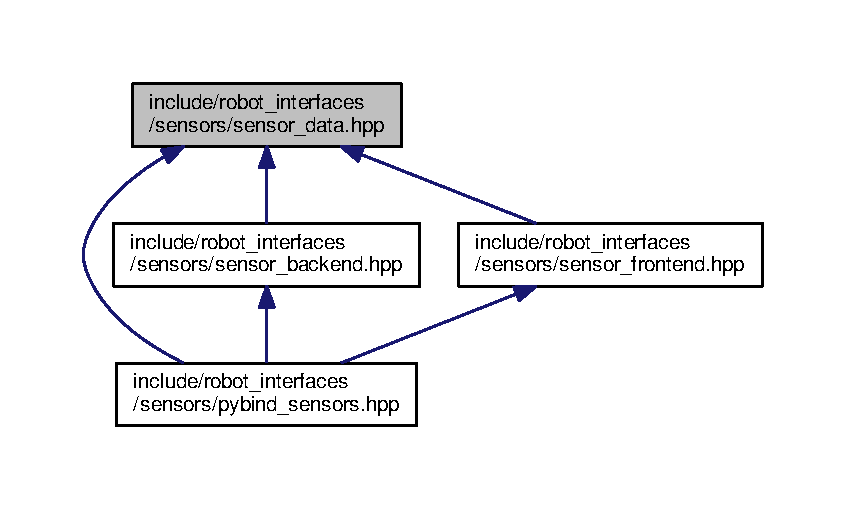
\includegraphics[width=350pt]{sensor__data_8hpp__dep__incl}
\end{center}
\end{figure}
\subsection*{Classes}
\begin{DoxyCompactItemize}
\item 
class \hyperlink{classrobot__interfaces_1_1SensorData}{robot\+\_\+interfaces\+::\+Sensor\+Data$<$ Observation\+Type $>$}
\begin{DoxyCompactList}\small\item\em Contains all the data coming from the sensors. \end{DoxyCompactList}\end{DoxyCompactItemize}


\subsection{Detailed Description}
To store all the data from all the sensors in use. 

\begin{DoxyCopyright}{Copyright}
2020, New York University, Max Planck Gesellschaft. All rights reserved. 
\end{DoxyCopyright}
\begin{DoxyRefDesc}{License}
\item[\hyperlink{license__license000006}{License}]B\+SD 3-\/clause \end{DoxyRefDesc}

\hypertarget{sensor__driver_8hpp}{}\section{include/robot\+\_\+interfaces/sensors/sensor\+\_\+driver.hpp File Reference}
\label{sensor__driver_8hpp}\index{include/robot\+\_\+interfaces/sensors/sensor\+\_\+driver.\+hpp@{include/robot\+\_\+interfaces/sensors/sensor\+\_\+driver.\+hpp}}


Base driver for the sensors.  


{\ttfamily \#include $<$iostream$>$}\\*
Include dependency graph for sensor\+\_\+driver.\+hpp\+:
\nopagebreak
\begin{figure}[H]
\begin{center}
\leavevmode
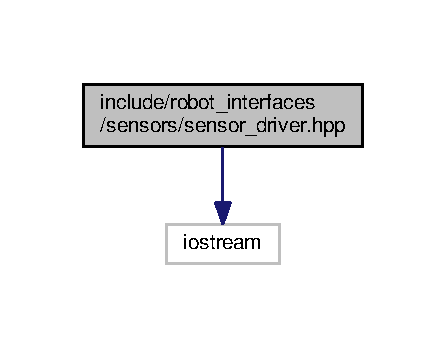
\includegraphics[width=214pt]{sensor__driver_8hpp__incl}
\end{center}
\end{figure}
This graph shows which files directly or indirectly include this file\+:
\nopagebreak
\begin{figure}[H]
\begin{center}
\leavevmode
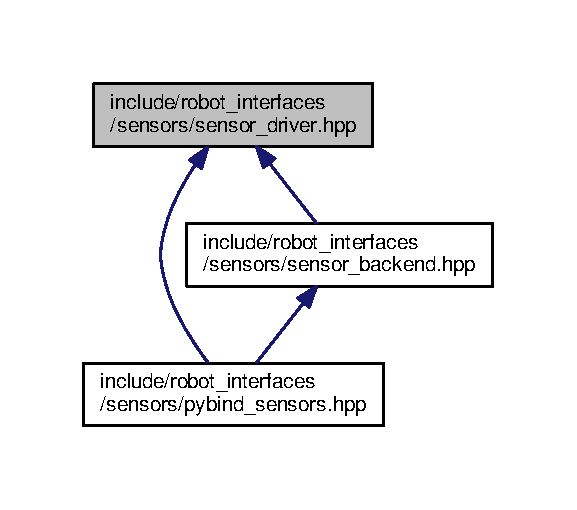
\includegraphics[width=277pt]{sensor__driver_8hpp__dep__incl}
\end{center}
\end{figure}
\subsection*{Classes}
\begin{DoxyCompactItemize}
\item 
class \hyperlink{classrobot__interfaces_1_1SensorDriver}{robot\+\_\+interfaces\+::\+Sensor\+Driver$<$ Observation\+Type $>$}
\begin{DoxyCompactList}\small\item\em Base driver class from which all specific sensor drivers should derive. \end{DoxyCompactList}\end{DoxyCompactItemize}


\subsection{Detailed Description}
Base driver for the sensors. 

\begin{DoxyCopyright}{Copyright}
2020, New York University, Max Planck Gesellschaft. All rights reserved. 
\end{DoxyCopyright}
\begin{DoxyRefDesc}{License}
\item[\hyperlink{license__license000007}{License}]B\+SD 3-\/clause \end{DoxyRefDesc}

\hypertarget{sensor__frontend_8hpp}{}\section{include/robot\+\_\+interfaces/sensors/sensor\+\_\+frontend.hpp File Reference}
\label{sensor__frontend_8hpp}\index{include/robot\+\_\+interfaces/sensors/sensor\+\_\+frontend.\+hpp@{include/robot\+\_\+interfaces/sensors/sensor\+\_\+frontend.\+hpp}}


Consists of methods that are exposed to the user to interact with the sensors.  


{\ttfamily \#include $<$algorithm$>$}\\*
{\ttfamily \#include $<$cmath$>$}\\*
{\ttfamily \#include $<$time\+\_\+series/time\+\_\+series.\+hpp$>$}\\*
{\ttfamily \#include $<$robot\+\_\+interfaces/sensors/sensor\+\_\+data.\+hpp$>$}\\*
Include dependency graph for sensor\+\_\+frontend.\+hpp\+:
\nopagebreak
\begin{figure}[H]
\begin{center}
\leavevmode
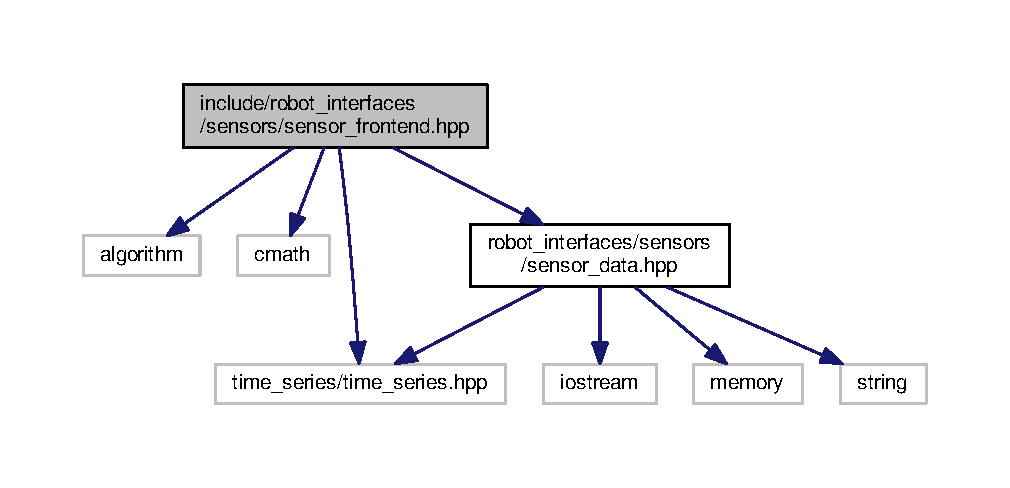
\includegraphics[width=350pt]{sensor__frontend_8hpp__incl}
\end{center}
\end{figure}
This graph shows which files directly or indirectly include this file\+:
\nopagebreak
\begin{figure}[H]
\begin{center}
\leavevmode
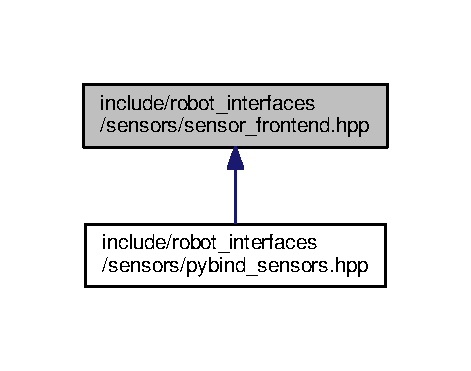
\includegraphics[width=226pt]{sensor__frontend_8hpp__dep__incl}
\end{center}
\end{figure}
\subsection*{Classes}
\begin{DoxyCompactItemize}
\item 
class \hyperlink{classrobot__interfaces_1_1SensorFrontend}{robot\+\_\+interfaces\+::\+Sensor\+Frontend$<$ Observation\+Type $>$}
\begin{DoxyCompactList}\small\item\em Communication link between \hyperlink{classrobot__interfaces_1_1SensorData}{Sensor\+Data} and the user. \end{DoxyCompactList}\end{DoxyCompactItemize}


\subsection{Detailed Description}
Consists of methods that are exposed to the user to interact with the sensors. 

\begin{DoxyCopyright}{Copyright}
2020, New York University, Max Planck Gesellschaft. All rights reserved. 
\end{DoxyCopyright}
\begin{DoxyRefDesc}{License}
\item[\hyperlink{license__license000008}{License}]B\+SD 3-\/clause \end{DoxyRefDesc}

\hypertarget{status_8hpp}{}\section{include/robot\+\_\+interfaces/status.hpp File Reference}
\label{status_8hpp}\index{include/robot\+\_\+interfaces/status.\+hpp@{include/robot\+\_\+interfaces/status.\+hpp}}


Defines the Status struct.  


{\ttfamily \#include $<$cereal/types/string.\+hpp$>$}\\*
{\ttfamily \#include $<$robot\+\_\+interfaces/loggable.\+hpp$>$}\\*
{\ttfamily \#include $<$string$>$}\\*
{\ttfamily \#include $<$vector$>$}\\*
Include dependency graph for status.\+hpp\+:
\nopagebreak
\begin{figure}[H]
\begin{center}
\leavevmode
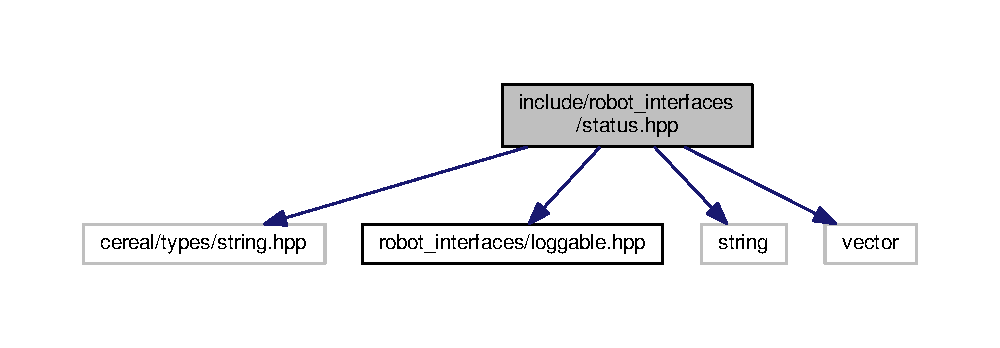
\includegraphics[width=350pt]{status_8hpp__incl}
\end{center}
\end{figure}
This graph shows which files directly or indirectly include this file\+:
\nopagebreak
\begin{figure}[H]
\begin{center}
\leavevmode
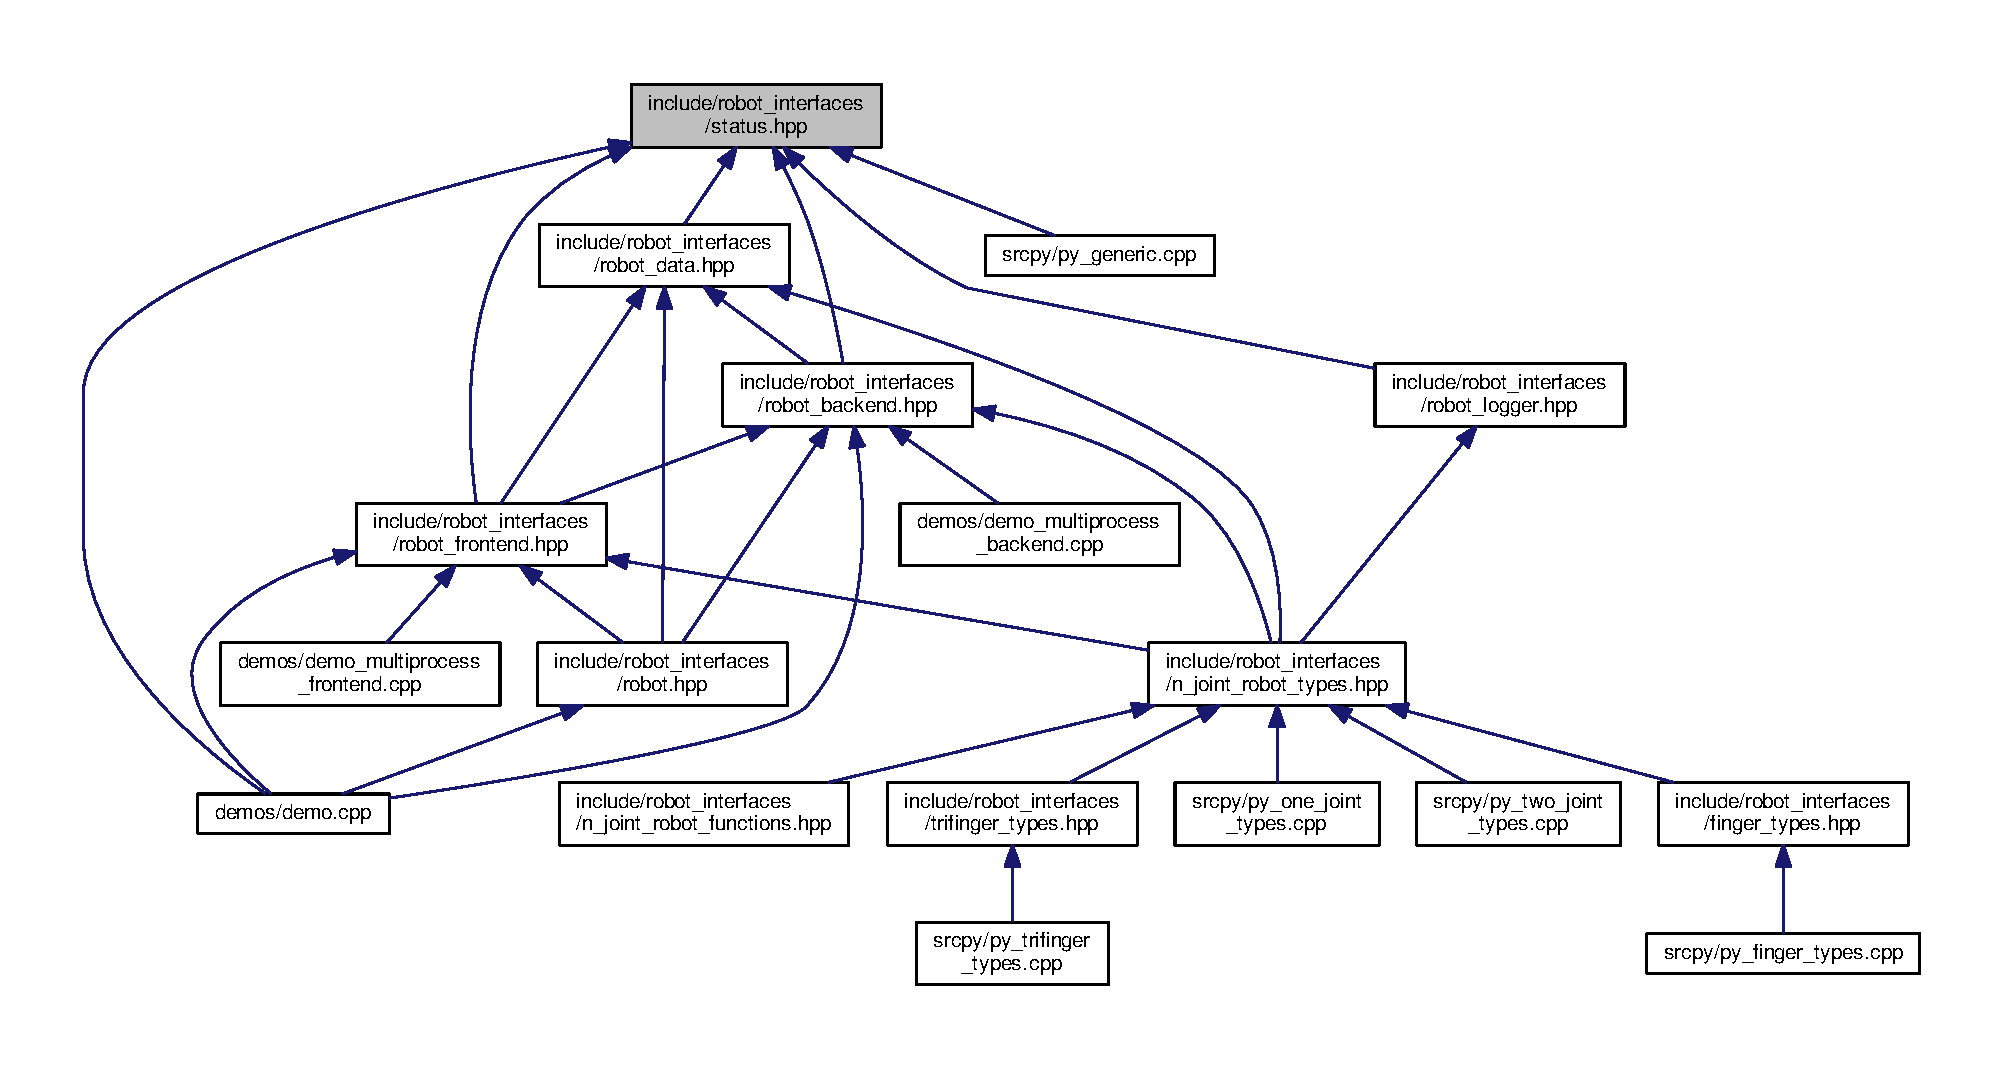
\includegraphics[width=350pt]{status_8hpp__dep__incl}
\end{center}
\end{figure}
\subsection*{Classes}
\begin{DoxyCompactItemize}
\item 
struct \hyperlink{structrobot__interfaces_1_1Status}{robot\+\_\+interfaces\+::\+Status}
\begin{DoxyCompactList}\small\item\em \hyperlink{structrobot__interfaces_1_1Status}{Status} information from the backend. \end{DoxyCompactList}\end{DoxyCompactItemize}


\subsection{Detailed Description}
Defines the Status struct. 


\hypertarget{global__signal__handler_8cpp}{}\section{src/global\+\_\+signal\+\_\+handler.cpp File Reference}
\label{global__signal__handler_8cpp}\index{src/global\+\_\+signal\+\_\+handler.\+cpp@{src/global\+\_\+signal\+\_\+handler.\+cpp}}
{\ttfamily \#include $<$csignal$>$}\\*
{\ttfamily \#include $<$robot\+\_\+interfaces/global\+\_\+signal\+\_\+handler.\+hpp$>$}\\*
Include dependency graph for global\+\_\+signal\+\_\+handler.\+cpp\+:
\nopagebreak
\begin{figure}[H]
\begin{center}
\leavevmode
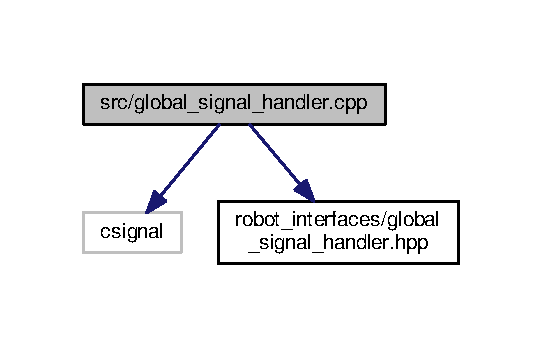
\includegraphics[width=260pt]{global__signal__handler_8cpp__incl}
\end{center}
\end{figure}


\subsection{Detailed Description}
\begin{DoxyCopyright}{Copyright}
2020, New York University, Max Planck Gesellschaft. All rights reserved. 
\end{DoxyCopyright}
\begin{DoxyRefDesc}{License}
\item[\hyperlink{license__license000009}{License}]B\+SD 3-\/clause \end{DoxyRefDesc}

\hypertarget{py__finger__types_8cpp}{}\section{srcpy/py\+\_\+finger\+\_\+types.cpp File Reference}
\label{py__finger__types_8cpp}\index{srcpy/py\+\_\+finger\+\_\+types.\+cpp@{srcpy/py\+\_\+finger\+\_\+types.\+cpp}}


Create bindings for One-\/\+Joint robot types.  


{\ttfamily \#include $<$robot\+\_\+interfaces/pybind\+\_\+helper.\+hpp$>$}\\*
{\ttfamily \#include $<$robot\+\_\+interfaces/finger\+\_\+types.\+hpp$>$}\\*
Include dependency graph for py\+\_\+finger\+\_\+types.\+cpp\+:
\nopagebreak
\begin{figure}[H]
\begin{center}
\leavevmode
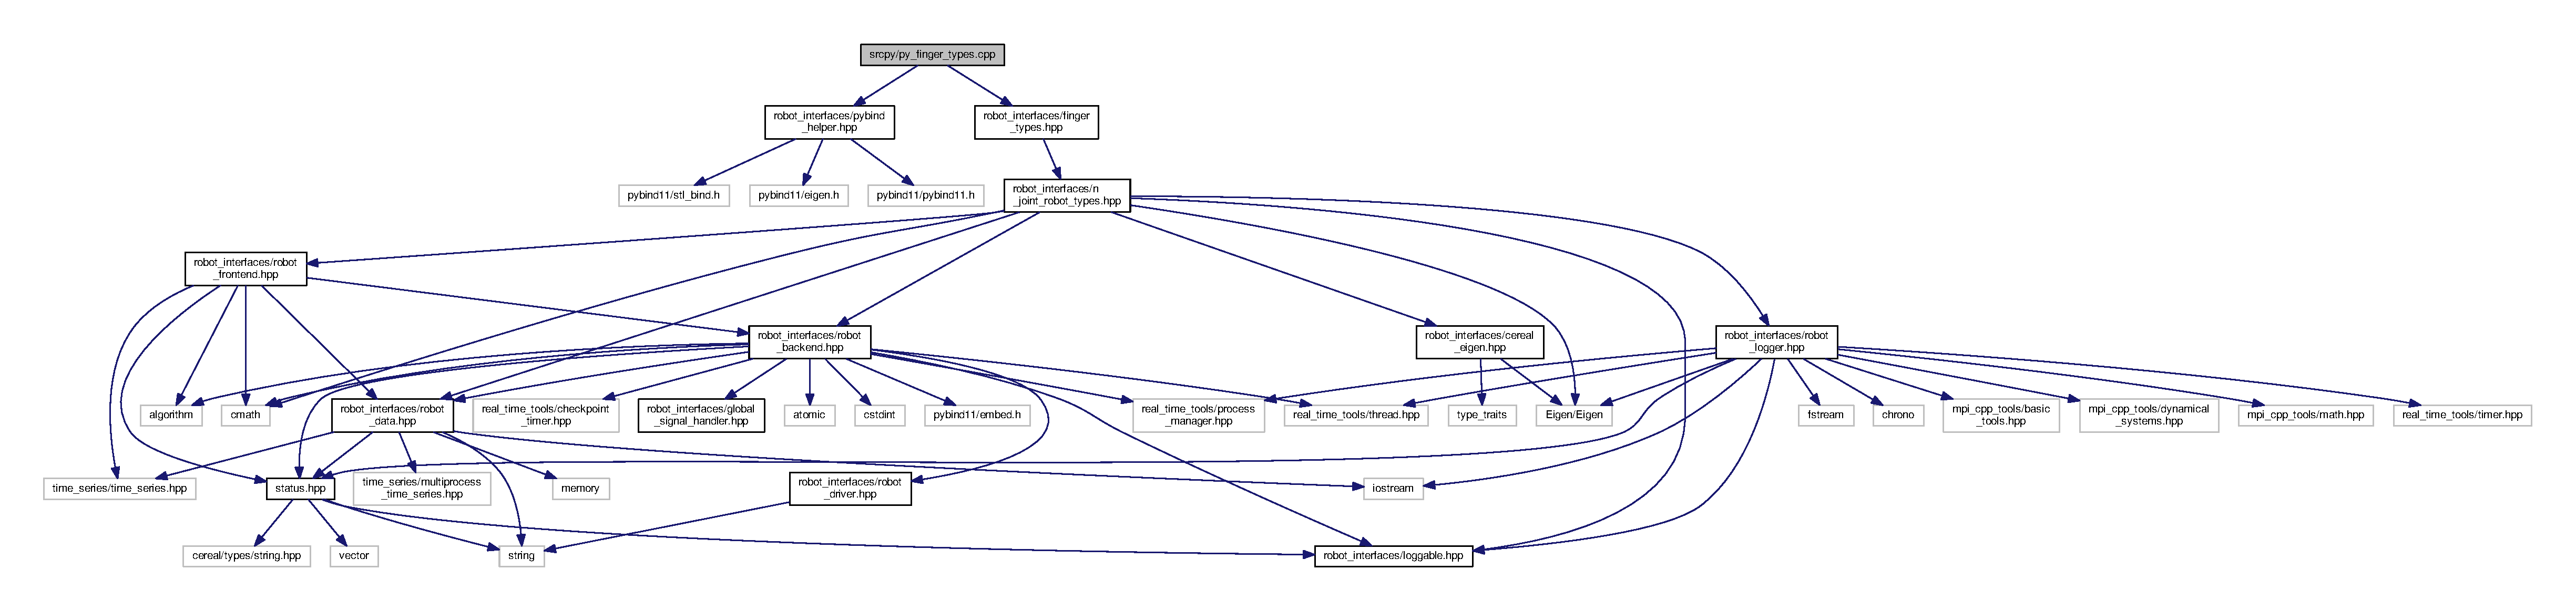
\includegraphics[width=350pt]{py__finger__types_8cpp__incl}
\end{center}
\end{figure}
\subsection*{Functions}
\begin{DoxyCompactItemize}
\item 
{\bfseries P\+Y\+B\+I\+N\+D11\+\_\+\+M\+O\+D\+U\+LE} (py\+\_\+finger\+\_\+types, m)\hypertarget{py__finger__types_8cpp_ab295ef4cf11fbedce6a7b19f4adb60e6}{}\label{py__finger__types_8cpp_ab295ef4cf11fbedce6a7b19f4adb60e6}

\end{DoxyCompactItemize}


\subsection{Detailed Description}
Create bindings for One-\/\+Joint robot types. 


\hypertarget{py__generic_8cpp}{}\section{srcpy/py\+\_\+generic.cpp File Reference}
\label{py__generic_8cpp}\index{srcpy/py\+\_\+generic.\+cpp@{srcpy/py\+\_\+generic.\+cpp}}


Create bindings for generic types.  


{\ttfamily \#include $<$robot\+\_\+interfaces/pybind\+\_\+helper.\+hpp$>$}\\*
{\ttfamily \#include $<$robot\+\_\+interfaces/status.\+hpp$>$}\\*
Include dependency graph for py\+\_\+generic.\+cpp\+:
\nopagebreak
\begin{figure}[H]
\begin{center}
\leavevmode
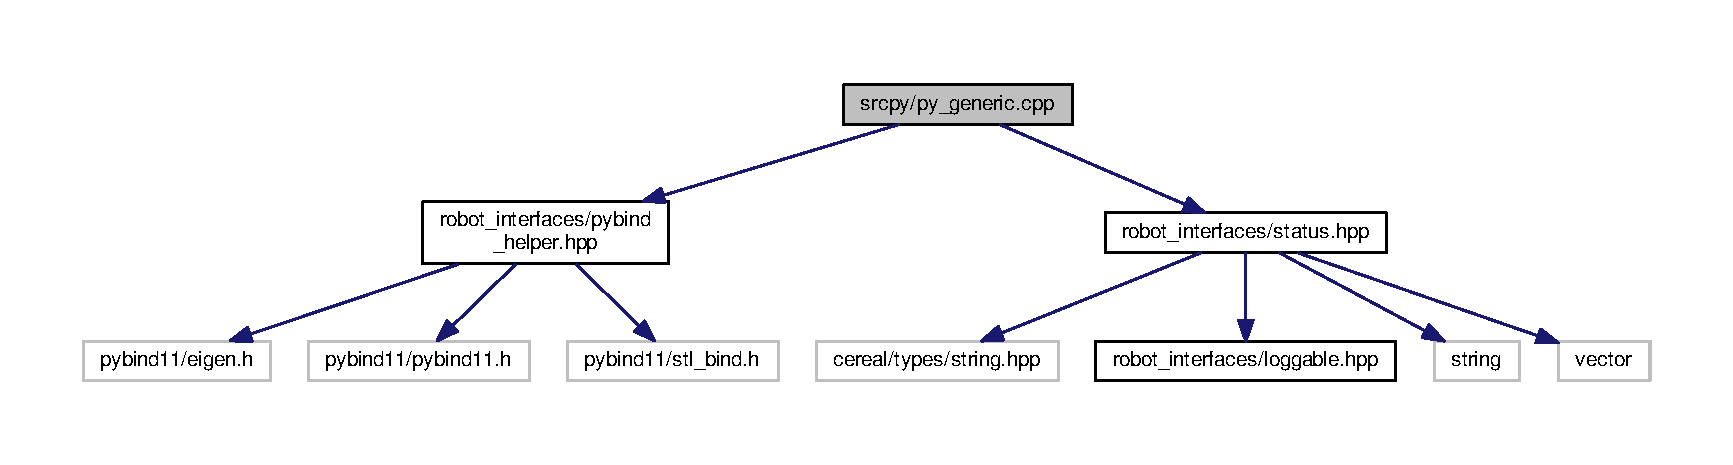
\includegraphics[width=350pt]{py__generic_8cpp__incl}
\end{center}
\end{figure}
\subsection*{Functions}
\begin{DoxyCompactItemize}
\item 
{\bfseries P\+Y\+B\+I\+N\+D11\+\_\+\+M\+O\+D\+U\+LE} (py\+\_\+generic, m)\hypertarget{py__generic_8cpp_a89eb84247e4a9479a3de283a82e9820f}{}\label{py__generic_8cpp_a89eb84247e4a9479a3de283a82e9820f}

\end{DoxyCompactItemize}


\subsection{Detailed Description}
Create bindings for generic types. 


\hypertarget{py__one__joint__types_8cpp}{}\section{srcpy/py\+\_\+one\+\_\+joint\+\_\+types.cpp File Reference}
\label{py__one__joint__types_8cpp}\index{srcpy/py\+\_\+one\+\_\+joint\+\_\+types.\+cpp@{srcpy/py\+\_\+one\+\_\+joint\+\_\+types.\+cpp}}


Create bindings for One-\/\+Joint robot types.  


{\ttfamily \#include $<$robot\+\_\+interfaces/pybind\+\_\+helper.\+hpp$>$}\\*
{\ttfamily \#include $<$robot\+\_\+interfaces/n\+\_\+joint\+\_\+robot\+\_\+types.\+hpp$>$}\\*
Include dependency graph for py\+\_\+one\+\_\+joint\+\_\+types.\+cpp\+:
\nopagebreak
\begin{figure}[H]
\begin{center}
\leavevmode
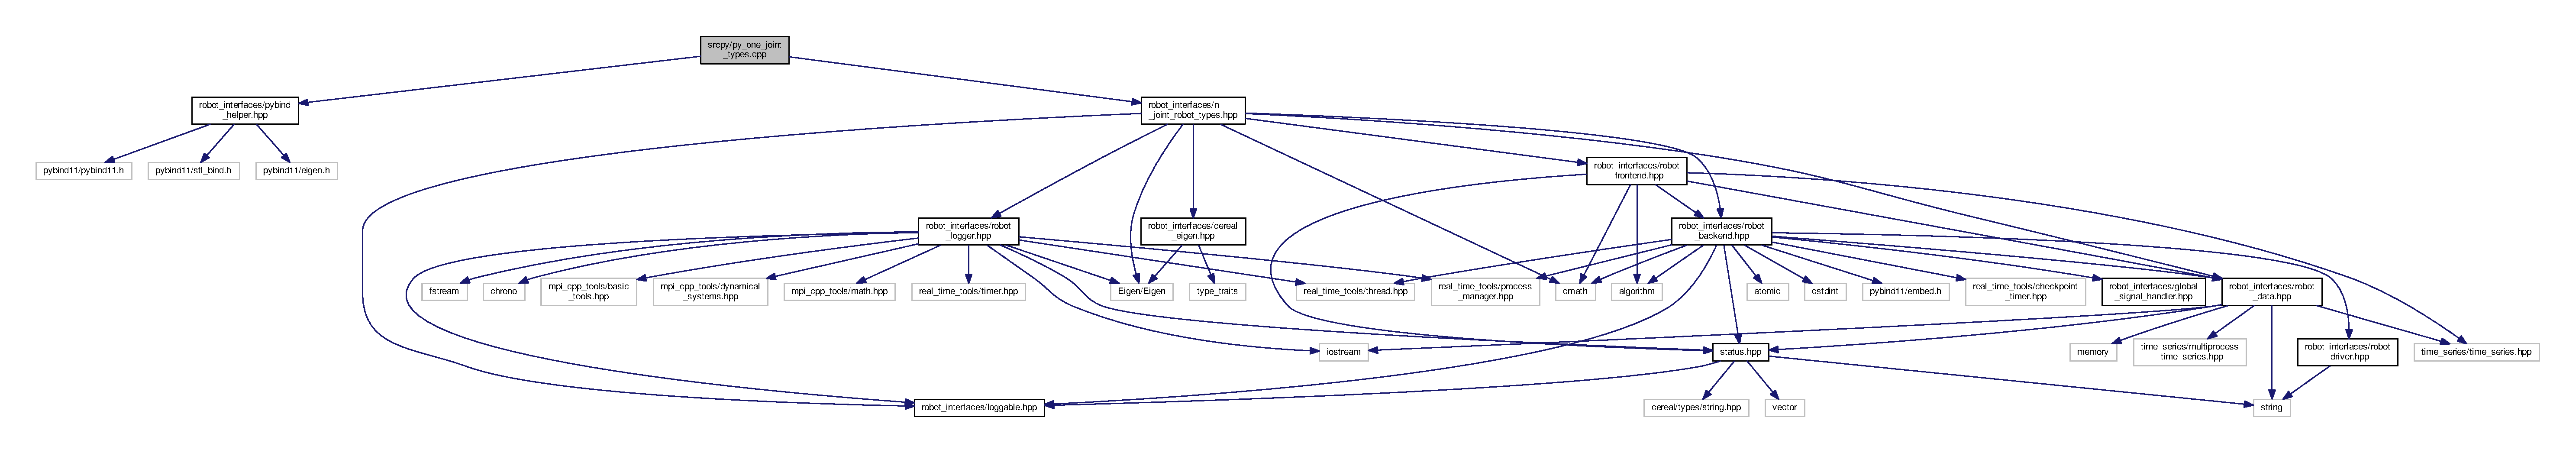
\includegraphics[width=350pt]{py__one__joint__types_8cpp__incl}
\end{center}
\end{figure}
\subsection*{Functions}
\begin{DoxyCompactItemize}
\item 
{\bfseries P\+Y\+B\+I\+N\+D11\+\_\+\+M\+O\+D\+U\+LE} (py\+\_\+one\+\_\+joint\+\_\+types, m)\hypertarget{py__one__joint__types_8cpp_a2c6ddd9ab0f0f91121b4fe0a3a9e0465}{}\label{py__one__joint__types_8cpp_a2c6ddd9ab0f0f91121b4fe0a3a9e0465}

\end{DoxyCompactItemize}


\subsection{Detailed Description}
Create bindings for One-\/\+Joint robot types. 


\hypertarget{py__trifinger__types_8cpp}{}\section{srcpy/py\+\_\+trifinger\+\_\+types.cpp File Reference}
\label{py__trifinger__types_8cpp}\index{srcpy/py\+\_\+trifinger\+\_\+types.\+cpp@{srcpy/py\+\_\+trifinger\+\_\+types.\+cpp}}


Create bindings for Tri\+Finger robot types.  


{\ttfamily \#include $<$robot\+\_\+interfaces/pybind\+\_\+helper.\+hpp$>$}\\*
{\ttfamily \#include $<$robot\+\_\+interfaces/trifinger\+\_\+types.\+hpp$>$}\\*
Include dependency graph for py\+\_\+trifinger\+\_\+types.\+cpp\+:
\nopagebreak
\begin{figure}[H]
\begin{center}
\leavevmode
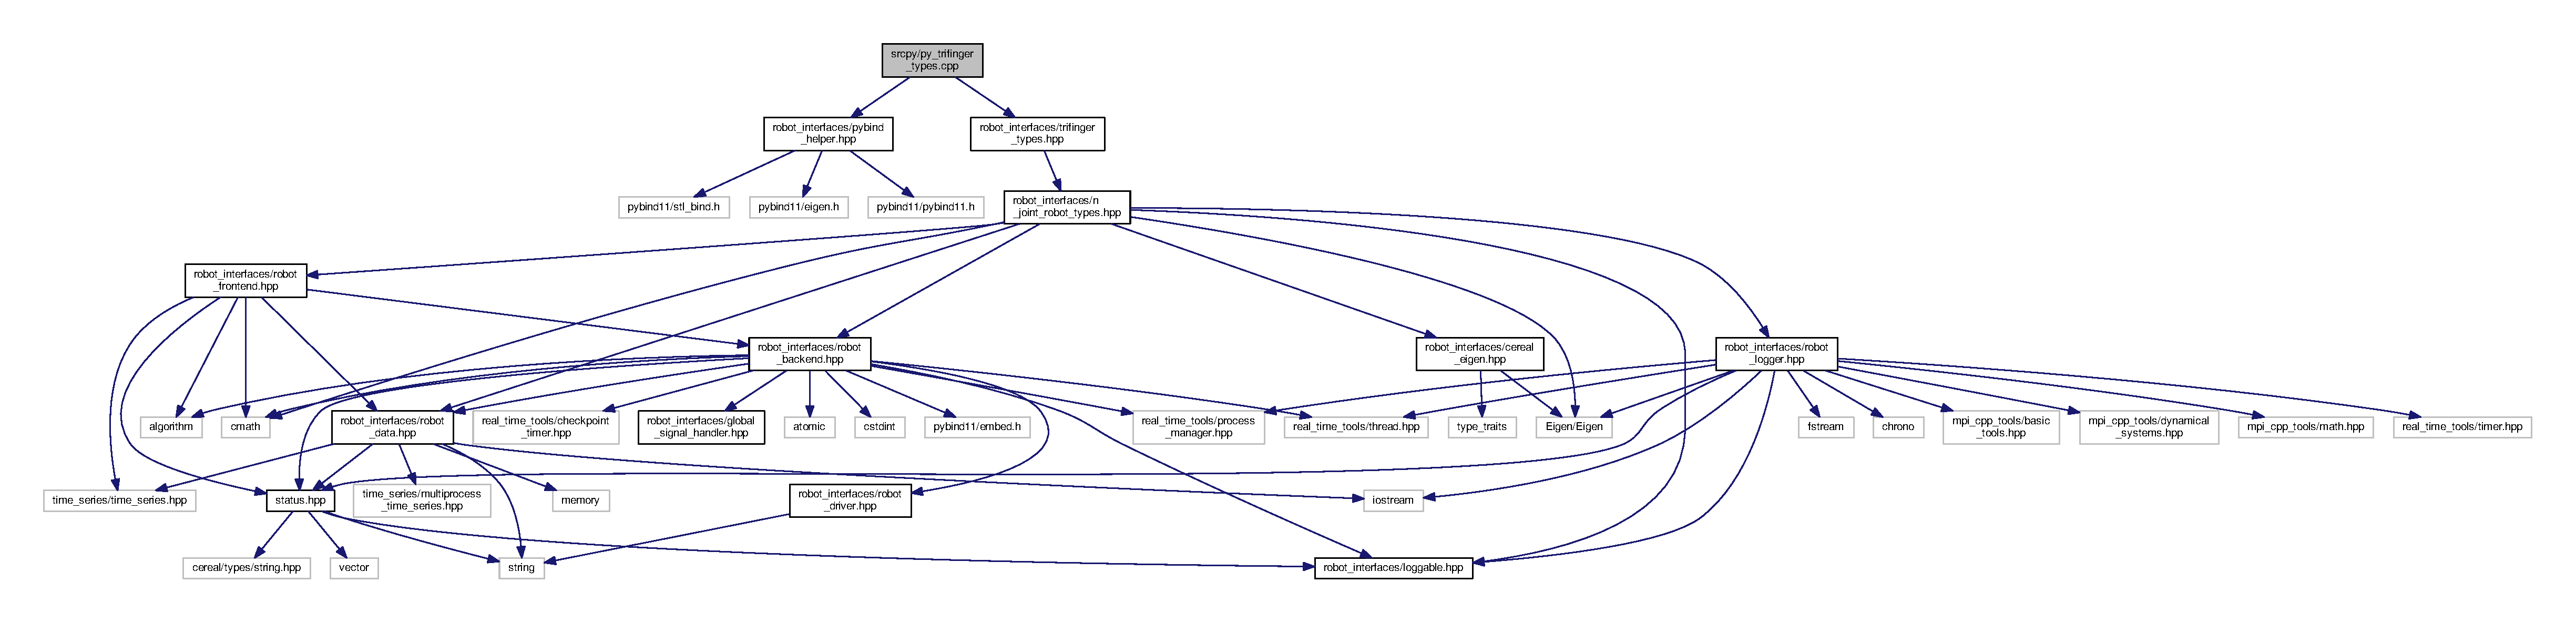
\includegraphics[width=350pt]{py__trifinger__types_8cpp__incl}
\end{center}
\end{figure}
\subsection*{Functions}
\begin{DoxyCompactItemize}
\item 
{\bfseries P\+Y\+B\+I\+N\+D11\+\_\+\+M\+O\+D\+U\+LE} (py\+\_\+trifinger\+\_\+types, m)\hypertarget{py__trifinger__types_8cpp_acde80b8029ae46e9e6a8d87c2f464d94}{}\label{py__trifinger__types_8cpp_acde80b8029ae46e9e6a8d87c2f464d94}

\end{DoxyCompactItemize}


\subsection{Detailed Description}
Create bindings for Tri\+Finger robot types. 


\hypertarget{py__two__joint__types_8cpp}{}\section{srcpy/py\+\_\+two\+\_\+joint\+\_\+types.cpp File Reference}
\label{py__two__joint__types_8cpp}\index{srcpy/py\+\_\+two\+\_\+joint\+\_\+types.\+cpp@{srcpy/py\+\_\+two\+\_\+joint\+\_\+types.\+cpp}}


Create bindings for Two-\/\+Joint robot types.  


{\ttfamily \#include $<$robot\+\_\+interfaces/pybind\+\_\+helper.\+hpp$>$}\\*
{\ttfamily \#include $<$robot\+\_\+interfaces/n\+\_\+joint\+\_\+robot\+\_\+types.\+hpp$>$}\\*
Include dependency graph for py\+\_\+two\+\_\+joint\+\_\+types.\+cpp\+:
\nopagebreak
\begin{figure}[H]
\begin{center}
\leavevmode
\includegraphics[width=350pt]{py__two__joint__types_8cpp__incl}
\end{center}
\end{figure}
\subsection*{Functions}
\begin{DoxyCompactItemize}
\item 
{\bfseries P\+Y\+B\+I\+N\+D11\+\_\+\+M\+O\+D\+U\+LE} (py\+\_\+two\+\_\+joint\+\_\+types, m)\hypertarget{py__two__joint__types_8cpp_a045f161d5577878718d68713b650463f}{}\label{py__two__joint__types_8cpp_a045f161d5577878718d68713b650463f}

\end{DoxyCompactItemize}


\subsection{Detailed Description}
Create bindings for Two-\/\+Joint robot types. 


\chapter{Example Documentation}
\hypertarget{demo_8cpp-example}{}\section{demo.\+cpp}
This demo shows robot\+\_\+interfaces of a dummy \char`\"{}2dof\char`\"{} robot, in which a dof \char`\"{}position\char`\"{} is represented by an integer


\begin{DoxyCodeInclude}

\textcolor{preprocessor}{#include "robot\_interfaces/monitored\_robot\_driver.hpp"}
\textcolor{preprocessor}{#include "robot\_interfaces/robot.hpp"}
\textcolor{preprocessor}{#include "robot\_interfaces/robot\_backend.hpp"}
\textcolor{preprocessor}{#include "robot\_interfaces/robot\_driver.hpp"}
\textcolor{preprocessor}{#include "robot\_interfaces/robot\_frontend.hpp"}
\textcolor{preprocessor}{#include "\hyperlink{status_8hpp}{robot\_interfaces/status.hpp}"}

\textcolor{preprocessor}{#include <memory>}

\textcolor{comment}{// Actions to be performed by robot, will be received by Driver}
\textcolor{comment}{// An action simply encapsulate two desired position value,}
\textcolor{comment}{// one for each dof}
\textcolor{keyword}{class }\hyperlink{classAction}{Action}
\{
\textcolor{keyword}{public}:
    \textcolor{keywordtype}{int} values[2];

    \textcolor{keywordtype}{void} print(\textcolor{keywordtype}{bool} backline)
    \{
        std::cout << \textcolor{stringliteral}{"action: "} << values[0] << \textcolor{stringliteral}{" "} << values[1] << \textcolor{stringliteral}{" "};
        \textcolor{keywordflow}{if} (backline) std::cout << \textcolor{stringliteral}{"\(\backslash\)n"};
    \}
\};

\textcolor{comment}{// Read from the robot by Driver}
\textcolor{comment}{// An observation is the current position}
\textcolor{comment}{// for each dof}
\textcolor{keyword}{class }\hyperlink{classObservation}{Observation}
\{
\textcolor{keyword}{public}:
    \textcolor{keywordtype}{int} values[2];

    \textcolor{keywordtype}{void} print(\textcolor{keywordtype}{bool} backline)
    \{
        std::cout << \textcolor{stringliteral}{"observation: "} << values[0] << \textcolor{stringliteral}{" "} << values[1] << \textcolor{stringliteral}{" "};
        \textcolor{keywordflow}{if} (backline) std::cout << \textcolor{stringliteral}{"\(\backslash\)n"};
    \}
\};

\textcolor{comment}{// Send command to the robot and read observation from the robot}
\textcolor{comment}{// The dof positions simply becomes the ones set by the latest action,}
\textcolor{comment}{// capped between a min and a max value (0 and 1000)}
\textcolor{keyword}{class }\hyperlink{classDriver}{Driver} : \textcolor{keyword}{public} \hyperlink{classrobot__interfaces_1_1RobotDriver}{robot\_interfaces::RobotDriver}<Action, Observation>
\{
\textcolor{keyword}{public}:
    \hyperlink{classDriver}{Driver}(\textcolor{keywordtype}{int} min, \textcolor{keywordtype}{int} max) : min\_(min), max\_(max)
    \{
    \}

    \textcolor{comment}{// at init dof are at min value}
    \textcolor{keywordtype}{void} initialize()
    \{
        state\_[0] = min\_;
        state\_[1] = min\_;
    \}

    \textcolor{comment}{// just clip desired values}
    \textcolor{comment}{// between 0 and 1000}
    \hyperlink{classAction}{Action} apply\_action(\textcolor{keyword}{const} \hyperlink{classAction}{Action} &action\_to\_apply)
    \{
        \hyperlink{classAction}{Action} applied;
        \textcolor{keywordflow}{for} (\textcolor{keywordtype}{unsigned} \textcolor{keywordtype}{int} i = 0; i < 2; i++)
        \{
            \textcolor{keywordflow}{if} (action\_to\_apply.values[i] > max\_)
            \{
                applied.values[i] = max\_;
            \}
            \textcolor{keywordflow}{else} \textcolor{keywordflow}{if} (action\_to\_apply.values[i] < min\_)
            \{
                applied.values[i] = min\_;
            \}
            \textcolor{keywordflow}{else}
            \{
                applied.values[i] = action\_to\_apply.values[i];
            \}
            \textcolor{comment}{// simulating the time if could take for a real}
            \textcolor{comment}{// robot to perform the action}
            usleep(1000);
            state\_[i] = applied.values[i];
        \}
        \textcolor{keywordflow}{return} applied;
    \}

    \hyperlink{classObservation}{Observation} get\_latest\_observation()
    \{
        \hyperlink{classObservation}{Observation} observation;
        observation.values[0] = state\_[0];
        observation.values[1] = state\_[1];
        \textcolor{keywordflow}{return} observation;
    \}

    std::string get\_error()
    \{
        \textcolor{keywordflow}{return} \textcolor{stringliteral}{""};  \textcolor{comment}{// no error}
    \}

    \textcolor{keywordtype}{void} shutdown()
    \{
    \}

\textcolor{keyword}{private}:
    \textcolor{keywordtype}{int} state\_[2];
    \textcolor{keywordtype}{int} min\_;
    \textcolor{keywordtype}{int} max\_;
\};

\textcolor{keywordtype}{int} main()
\{
    \textcolor{keyword}{typedef} \hyperlink{classrobot__interfaces_1_1RobotBackend}{robot\_interfaces::RobotBackend<Action, Observation>}
       Backend;
    \textcolor{keyword}{typedef} \hyperlink{classrobot__interfaces_1_1SingleProcessRobotData}{robot\_interfaces::SingleProcessRobotData<Action, Observation>}
       Data;
    \textcolor{keyword}{typedef} \hyperlink{classrobot__interfaces_1_1RobotFrontend}{robot\_interfaces::RobotFrontend<Action, Observation>}
       Frontend;

    \textcolor{comment}{// max time allowed for the robot to apply an action.}
    \textcolor{keywordtype}{double} max\_action\_duration\_s = 0.02;

    \textcolor{comment}{// max time allowed for 2 successive actions}
    \textcolor{keywordtype}{double} max\_inter\_action\_duration\_s = 0.05;

    \textcolor{comment}{// demo showing the separated usage of backend and frontend}
    \{
        std::cout << \textcolor{stringliteral}{"\(\backslash\)n -- * -- Frontend and Backend -- * --\(\backslash\)n"} << std::endl;

        std::shared\_ptr<Driver> driver\_ptr = std::make\_shared<Driver>(0, 1000);
        \textcolor{comment}{// Wrap the driver in a MonitoredRobotDriver to automatically run a}
        \textcolor{comment}{// timing watchdog.  If timing is violated, the robot will immediately}
        \textcolor{comment}{// be shut down.}
        \textcolor{comment}{// If no time monitoring is needed in your application, you can simply}
        \textcolor{comment}{// use the `driver\_ptr` directly, without the wrapper.}
        \textcolor{keyword}{auto} monitored\_driver\_ptr = std::make\_shared<
            \hyperlink{classrobot__interfaces_1_1MonitoredRobotDriver}{robot\_interfaces::MonitoredRobotDriver<Driver>}>(
            driver\_ptr, max\_action\_duration\_s, max\_inter\_action\_duration\_s);

        std::shared\_ptr<Data> data\_ptr = std::make\_shared<Data>();

        Backend backend(monitored\_driver\_ptr, data\_ptr);
        backend.initialize();

        Frontend frontend(data\_ptr);

        \hyperlink{classAction}{Action} action;
        \hyperlink{classObservation}{Observation} observation;

        \textcolor{comment}{// simulated action :}
        \textcolor{comment}{// 1 dof going from 200 to 300}
        \textcolor{comment}{// The other going from 300 to 200}

        \textcolor{keywordflow}{for} (uint value = 200; value <= 300; value++)
        \{
            action.values[0] = value;
            action.values[1] = 500 - value;
            \textcolor{comment}{// this action will be stored at index}
            robot\_interfaces::TimeIndex index =
                frontend.append\_desired\_action(action);
            \textcolor{comment}{// getting the observation corresponding to the applied}
            \textcolor{comment}{// action, i.e. at the same index}
            observation = frontend.get\_observation(index);
            std::cout << \textcolor{stringliteral}{"value: "} << value << \textcolor{stringliteral}{" | "};
            action.print(\textcolor{keyword}{false});
            observation.print(\textcolor{keyword}{true});
        \}
    \}

    \textcolor{comment}{// demo representing usage of frontend and backend}
    \textcolor{comment}{// encapsulated in the same instance}
    \{
        std::cout << \textcolor{stringliteral}{"\(\backslash\)n -- * -- Robot -- * --\(\backslash\)n"} << std::endl;

        \textcolor{keyword}{typedef} \hyperlink{classrobot__interfaces_1_1Robot}{robot\_interfaces::Robot<Action, Observation, Driver>}
       Robot;

        \textcolor{keywordtype}{int} min = 0;
        \textcolor{keywordtype}{int} max = 100;
        Robot robot(
            max\_action\_duration\_s, max\_inter\_action\_duration\_s, min, max);

        robot.initialize();

        \hyperlink{classAction}{Action} action;
        \hyperlink{classObservation}{Observation} observation;

        \textcolor{comment}{// simulated action :}
        \textcolor{comment}{// 1 dof going from 200 to 300}
        \textcolor{comment}{// The other going from 300 to 200}

        \textcolor{keywordflow}{for} (uint value = 200; value <= 300; value++)
        \{
            action.values[0] = value;
            action.values[1] = 500 - value;
            \textcolor{comment}{// this action will be stored at index}
            robot\_interfaces::TimeIndex index =
                robot.append\_desired\_action(action);
            \textcolor{comment}{// getting the observation corresponding to the applied}
            \textcolor{comment}{// action, i.e. at the same index}
            observation = robot.get\_observation(index);
            std::cout << \textcolor{stringliteral}{"value: "} << value << \textcolor{stringliteral}{" | "};
            action.print(\textcolor{keyword}{false});
            observation.print(\textcolor{keyword}{true});
        \}
    \}
\}
\end{DoxyCodeInclude}
 
\hypertarget{demo_multiprocess_backend_8cpp-example}{}\section{demo\+\_\+multiprocess\+\_\+backend.\+cpp}
Robot backend for a dummy \char`\"{}2dof\char`\"{} robot in a multi process setup.


\begin{DoxyCodeInclude}

\textcolor{preprocessor}{#include <memory>}

\textcolor{preprocessor}{#include "robot\_interfaces/robot\_backend.hpp"}
\textcolor{preprocessor}{#include "robot\_interfaces/robot\_driver.hpp"}

\textcolor{preprocessor}{#include "\hyperlink{types_8hpp}{types.hpp}"}

\textcolor{keyword}{using namespace }\hyperlink{namespacerobot__interfaces_1_1demo}{robot\_interfaces::demo};

\textcolor{comment}{// TODO put driver in separate file so no duplication to demo.cpp?  Discuss}
\textcolor{comment}{// with Vincent.}

\textcolor{comment}{// Send command to the robot and read observation from the robot}
\textcolor{comment}{// The dof positions simply becomes the ones set by the latest action,}
\textcolor{comment}{// capped between a min and a max value (0 and 1000)}
\textcolor{keyword}{class }\hyperlink{classDriver}{Driver} : \textcolor{keyword}{public} \hyperlink{classrobot__interfaces_1_1RobotDriver}{robot\_interfaces::RobotDriver}<Action, Observation>
\{
\textcolor{keyword}{public}:
    \hyperlink{classDriver}{Driver}()
    \{
    \}

    \textcolor{comment}{// at init dof are at min value}
    \textcolor{keywordtype}{void} initialize()
    \{
        state\_[0] = Driver::MIN;
        state\_[1] = Driver::MIN;
    \}

    \textcolor{comment}{// just clip desired values}
    \textcolor{comment}{// between 0 and 1000}
    \hyperlink{classrobot__interfaces_1_1demo_1_1Action}{Action} apply\_action(\textcolor{keyword}{const} \hyperlink{classrobot__interfaces_1_1demo_1_1Action}{Action} &action\_to\_apply)
    \{
        std::cout << \textcolor{stringliteral}{"received action "};
        action\_to\_apply.print(\textcolor{keyword}{true});

        \hyperlink{classrobot__interfaces_1_1demo_1_1Action}{Action} applied;
        \textcolor{keywordflow}{for} (\textcolor{keywordtype}{unsigned} \textcolor{keywordtype}{int} i = 0; i < 2; i++)
        \{
            \textcolor{keywordflow}{if} (action\_to\_apply.values[i] > Driver::MAX)
            \{
                applied.values[i] = Driver::MAX;
            \}
            \textcolor{keywordflow}{else} \textcolor{keywordflow}{if} (action\_to\_apply.values[i] < Driver::MIN)
            \{
                applied.values[i] = Driver::MIN;
            \}
            \textcolor{keywordflow}{else}
            \{
                applied.values[i] = action\_to\_apply.values[i];
            \}
            \textcolor{comment}{// simulating the time if could take for a real}
            \textcolor{comment}{// robot to perform the action}
            usleep(1000);
            state\_[i] = applied.values[i];
        \}
        \textcolor{keywordflow}{return} applied;
    \}

    \hyperlink{classrobot__interfaces_1_1demo_1_1Observation}{Observation} get\_latest\_observation()
    \{
        \hyperlink{classrobot__interfaces_1_1demo_1_1Observation}{Observation} observation;
        observation.values[0] = state\_[0];
        observation.values[1] = state\_[1];
        \textcolor{keywordflow}{return} observation;
    \}

    std::string get\_error()
    \{
        \textcolor{keywordflow}{return} \textcolor{stringliteral}{""};  \textcolor{comment}{// no error}
    \}

    \textcolor{keywordtype}{void} shutdown()
    \{
        \textcolor{comment}{// nothing to do}
    \}

\textcolor{keyword}{private}:
    \textcolor{keywordtype}{int} state\_[2];

    \textcolor{keyword}{const} \textcolor{keyword}{static} \textcolor{keywordtype}{int} MAX = 1000;
    \textcolor{keyword}{const} \textcolor{keyword}{static} \textcolor{keywordtype}{int} MIN = 0;
\};

\textcolor{keywordtype}{int} main()
\{
    \textcolor{keyword}{typedef} \hyperlink{classrobot__interfaces_1_1RobotBackend}{robot\_interfaces::RobotBackend<Action, Observation>}
       Backend;
    \textcolor{keyword}{typedef} \hyperlink{classrobot__interfaces_1_1MultiProcessRobotData}{robot\_interfaces::MultiProcessRobotData<Action, Observation>}
        MultiProcessData;

    \textcolor{keyword}{auto} driver\_ptr = std::make\_shared<Driver>();
    \textcolor{comment}{// the backend process acts as master for the shared memory}
    \textcolor{keyword}{auto} data\_ptr =
        std::make\_shared<MultiProcessData>(\textcolor{stringliteral}{"multiprocess\_demo"}, \textcolor{keyword}{true});

    Backend backend(driver\_ptr, data\_ptr);
    backend.initialize();

    \textcolor{comment}{// TODO would be nicer to check if backend loop is still running}
    \textcolor{keywordflow}{while} (\textcolor{keyword}{true})
    \{
    \}
\}

\end{DoxyCodeInclude}
 
\hypertarget{demo_multiprocess_frontend_8cpp-example}{}\section{demo\+\_\+multiprocess\+\_\+frontend.\+cpp}
Robot frontend for a dummy \char`\"{}2dof\char`\"{} robot in a multi process setup.


\begin{DoxyCodeInclude}

\textcolor{preprocessor}{#include <memory>}

\textcolor{preprocessor}{#include "robot\_interfaces/robot\_frontend.hpp"}

\textcolor{preprocessor}{#include "\hyperlink{types_8hpp}{types.hpp}"}

\textcolor{keyword}{using namespace }\hyperlink{namespacerobot__interfaces_1_1demo}{robot\_interfaces::demo};

\textcolor{keywordtype}{int} main()
\{
    \textcolor{keyword}{typedef} \hyperlink{classrobot__interfaces_1_1RobotFrontend}{robot\_interfaces::RobotFrontend<Action, Observation>}
       Frontend;
    \textcolor{keyword}{typedef} \hyperlink{classrobot__interfaces_1_1MultiProcessRobotData}{robot\_interfaces::MultiProcessRobotData<Action, Observation>}
        MultiProcessData;

    \textcolor{comment}{// The shared memory is managed by the backend process, so set the}
    \textcolor{comment}{// is\_master argument to false.}
    \textcolor{keyword}{auto} data\_ptr =
        std::make\_shared<MultiProcessData>(\textcolor{stringliteral}{"multiprocess\_demo"}, \textcolor{keyword}{false});
    Frontend frontend(data\_ptr);

    \hyperlink{classrobot__interfaces_1_1demo_1_1Action}{Action} action;
    \hyperlink{classrobot__interfaces_1_1demo_1_1Observation}{Observation} observation;

    \textcolor{comment}{// simulated action :}
    \textcolor{comment}{// 1 dof going from 200 to 300}
    \textcolor{comment}{// The other going from 300 to 200}

    \textcolor{keywordflow}{for} (uint value = 200; value <= 300; value++)
    \{
        action.values[0] = value;
        action.values[1] = 500 - value;
        \textcolor{comment}{// this action will be stored at index}
        robot\_interfaces::TimeIndex index =
            frontend.append\_desired\_action(action);
        \textcolor{comment}{// getting the observation corresponding to the applied}
        \textcolor{comment}{// action, i.e. at the same index}
        observation = frontend.get\_observation(index);
        std::cout << \textcolor{stringliteral}{"value: "} << value << \textcolor{stringliteral}{" | "};
        action.print(\textcolor{keyword}{false});
        observation.print(\textcolor{keyword}{true});
    \}
\}

\end{DoxyCodeInclude}
 
%--- End generated contents ---

% Index
\backmatter
\newpage
\phantomsection
\clearemptydoublepage
\addcontentsline{toc}{chapter}{Index}
\printindex

\end{document}
